\documentclass{article}\usepackage[]{graphicx}\usepackage[]{color}
%% maxwidth is the original width if it is less than linewidth
%% otherwise use linewidth (to make sure the graphics do not exceed the margin)
\makeatletter
\def\maxwidth{ %
  \ifdim\Gin@nat@width>\linewidth
    \linewidth
  \else
    \Gin@nat@width
  \fi
}
\makeatother

\definecolor{fgcolor}{rgb}{0.345, 0.345, 0.345}
\newcommand{\hlnum}[1]{\textcolor[rgb]{0.686,0.059,0.569}{#1}}%
\newcommand{\hlstr}[1]{\textcolor[rgb]{0.192,0.494,0.8}{#1}}%
\newcommand{\hlcom}[1]{\textcolor[rgb]{0.678,0.584,0.686}{\textit{#1}}}%
\newcommand{\hlopt}[1]{\textcolor[rgb]{0,0,0}{#1}}%
\newcommand{\hlstd}[1]{\textcolor[rgb]{0.345,0.345,0.345}{#1}}%
\newcommand{\hlkwa}[1]{\textcolor[rgb]{0.161,0.373,0.58}{\textbf{#1}}}%
\newcommand{\hlkwb}[1]{\textcolor[rgb]{0.69,0.353,0.396}{#1}}%
\newcommand{\hlkwc}[1]{\textcolor[rgb]{0.333,0.667,0.333}{#1}}%
\newcommand{\hlkwd}[1]{\textcolor[rgb]{0.737,0.353,0.396}{\textbf{#1}}}%
\let\hlipl\hlkwb

\usepackage{framed}
\makeatletter
\newenvironment{kframe}{%
 \def\at@end@of@kframe{}%
 \ifinner\ifhmode%
  \def\at@end@of@kframe{\end{minipage}}%
  \begin{minipage}{\columnwidth}%
 \fi\fi%
 \def\FrameCommand##1{\hskip\@totalleftmargin \hskip-\fboxsep
 \colorbox{shadecolor}{##1}\hskip-\fboxsep
     % There is no \\@totalrightmargin, so:
     \hskip-\linewidth \hskip-\@totalleftmargin \hskip\columnwidth}%
 \MakeFramed {\advance\hsize-\width
   \@totalleftmargin\z@ \linewidth\hsize
   \@setminipage}}%
 {\par\unskip\endMakeFramed%
 \at@end@of@kframe}
\makeatother

\definecolor{shadecolor}{rgb}{.97, .97, .97}
\definecolor{messagecolor}{rgb}{0, 0, 0}
\definecolor{warningcolor}{rgb}{1, 0, 1}
\definecolor{errorcolor}{rgb}{1, 0, 0}
\newenvironment{knitrout}{}{} % an empty environment to be redefined in TeX

\usepackage{alltt}
\usepackage{float}
\usepackage[parfill]{parskip}
\hbadness=10000
\IfFileExists{upquote.sty}{\usepackage{upquote}}{}
\begin{document}

\title{Coursework (CM3111)\\Big Data Analytics}
\author{Alistair Quinn}
\maketitle 

\par\noindent\rule{\textwidth}{0.4pt}

\section{Data Exploration}
\subsection{Dataset Choice}
I have chosen a dataset that was used in the CoIL 2000 Challenge, which is called the Caravan Insurance Challenge dataset available here: https://www.kaggle.com/uciml/caravan-insurance-challenge 

The data set is free to use for non-comercial use. Although sourced from the UCL Machine Learning organization's kaggle page, the dataset is owned by Sentient Machine Research. 
\subsection{Technology-Platform}
The dataset is contained in a csv file that is 245KB in size. As the dataset is so small I not need to use Big Data technology such as Hadoop. Instead I will use RStudio on a windows PC. I chose the dataset based on my current ability, and I found the idea of the dataset interesting. 
\subsection{Problem Statement & Data Exploration}
Each row in the table corresponds to a post code.The task with this dataset is to identify potential purchasers of caravan insurance policies. The class label in the dataset is called CARAVAN and has two values, 0 or 1. CARAVARN is 1 when that row would potentially purchase a caravan insurance policy. 

First I'll load the dataset I'm using.
\begin{knitrout}
\definecolor{shadecolor}{rgb}{0.969, 0.969, 0.969}\color{fgcolor}\begin{kframe}
\begin{alltt}
\hlcom{#Set WD}
\hlkwd{setwd}\hlstd{(}\hlstr{"D:/RGU/3rdYear/Semester1/Big Data Analytics/Coursework/wd"}\hlstd{)}
\hlcom{#Load Data}
\hlstd{df} \hlkwb{<-} \hlkwd{read.csv}\hlstd{(}\hlstr{"Data/caravan-insurance-challenge.csv"}\hlstd{)}
\end{alltt}
\end{kframe}
\end{knitrout}
I will now explore my dataset to identify its features and learn more about it. 

During my data exploration, I will be visualising my data using a package called ggplot2. This is a plotting system for R. I have chosen to use this package as I have experience with it from the labs in the course. It has some powerful plotting functions, and works in an intuative way. 
\begin{knitrout}
\definecolor{shadecolor}{rgb}{0.969, 0.969, 0.969}\color{fgcolor}\begin{kframe}
\begin{alltt}
\hlkwd{library}\hlstd{(ggplot2)}
\end{alltt}


{\ttfamily\noindent\color{warningcolor}{\#\# Warning: package 'ggplot2' was built under R version 3.4.2}}\end{kframe}
\end{knitrout}

Going to take a look at the number of rows and columns
\begin{knitrout}
\definecolor{shadecolor}{rgb}{0.969, 0.969, 0.969}\color{fgcolor}\begin{kframe}
\begin{alltt}
\hlcom{#Rows and Cols}
\hlkwd{nrow}\hlstd{(df)}
\end{alltt}
\begin{verbatim}
## [1] 9822
\end{verbatim}
\begin{alltt}
\hlkwd{ncol}\hlstd{(df)}
\end{alltt}
\begin{verbatim}
## [1] 87
\end{verbatim}
\end{kframe}
\end{knitrout}
There are currently 9822 rows, and 87 columns in the dataset 

Going to take a look at the features of the dataset
\begin{knitrout}
\definecolor{shadecolor}{rgb}{0.969, 0.969, 0.969}\color{fgcolor}\begin{kframe}
\begin{alltt}
\hlcom{#Names of columns }
\hlkwd{names}\hlstd{(df)}
\end{alltt}
\begin{verbatim}
##  [1] "ORIGIN"   "MOSTYPE"  "MAANTHUI" "MGEMOMV"  "MGEMLEEF" "MOSHOOFD"
##  [7] "MGODRK"   "MGODPR"   "MGODOV"   "MGODGE"   "MRELGE"   "MRELSA"  
## [13] "MRELOV"   "MFALLEEN" "MFGEKIND" "MFWEKIND" "MOPLHOOG" "MOPLMIDD"
## [19] "MOPLLAAG" "MBERHOOG" "MBERZELF" "MBERBOER" "MBERMIDD" "MBERARBG"
## [25] "MBERARBO" "MSKA"     "MSKB1"    "MSKB2"    "MSKC"     "MSKD"    
## [31] "MHHUUR"   "MHKOOP"   "MAUT1"    "MAUT2"    "MAUT0"    "MZFONDS" 
## [37] "MZPART"   "MINKM30"  "MINK3045" "MINK4575" "MINK7512" "MINK123M"
## [43] "MINKGEM"  "MKOOPKLA" "PWAPART"  "PWABEDR"  "PWALAND"  "PPERSAUT"
## [49] "PBESAUT"  "PMOTSCO"  "PVRAAUT"  "PAANHANG" "PTRACTOR" "PWERKT"  
## [55] "PBROM"    "PLEVEN"   "PPERSONG" "PGEZONG"  "PWAOREG"  "PBRAND"  
## [61] "PZEILPL"  "PPLEZIER" "PFIETS"   "PINBOED"  "PBYSTAND" "AWAPART" 
## [67] "AWABEDR"  "AWALAND"  "APERSAUT" "ABESAUT"  "AMOTSCO"  "AVRAAUT" 
## [73] "AAANHANG" "ATRACTOR" "AWERKT"   "ABROM"    "ALEVEN"   "APERSONG"
## [79] "AGEZONG"  "AWAOREG"  "ABRAND"   "AZEILPL"  "APLEZIER" "AFIETS"  
## [85] "AINBOED"  "ABYSTAND" "CARAVAN"
\end{verbatim}
\end{kframe}
\end{knitrout}
Variables beginning with M are demographic statistics of the postal code. 
\begin{figure}[H]
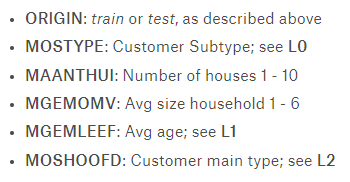
\includegraphics{images/mainfields.png}}
\end{figure}
Variables beginning with P and A refer to product ownership and insurance statistics of the postal code. Variables beginning with P refer to contribution policies. 
\begin{figure}[H]
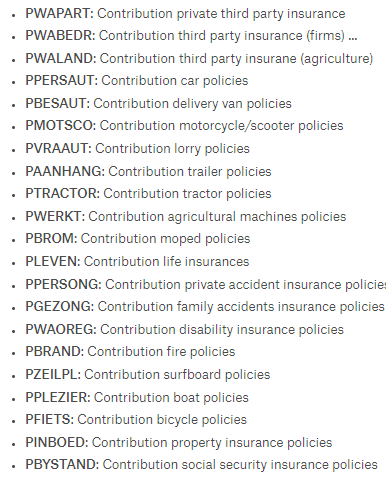
\includegraphics{images/contributionfields.png}
\end{figure}
variables beggining with A refer to number of policies.
\begin{figure}[H]
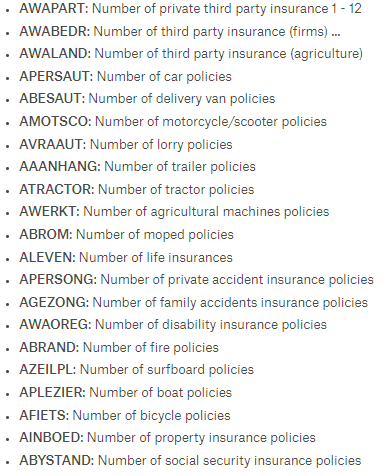
\includegraphics{images/numberoffields.png}
\end{figure}
Going to check the factors of the dataset
\begin{knitrout}
\definecolor{shadecolor}{rgb}{0.969, 0.969, 0.969}\color{fgcolor}\begin{kframe}
\begin{alltt}
\hlcom{#Names of columns }
\hlkwd{sapply}\hlstd{(df,levels)}
\end{alltt}
\end{kframe}
\end{knitrout}
I have ommited the result of the above code, as it was far too large. Most of the columns in the current data are numeric values but are actually supposed to be factors. I will refactor these columns during pre-processing. The only variable that has been turned into a factor by R is the first one, ORIGIN. I will explore this factor later. 

There are 4 keys that relate to this datset. A key for customer subtype:
\begin{figure}[H]
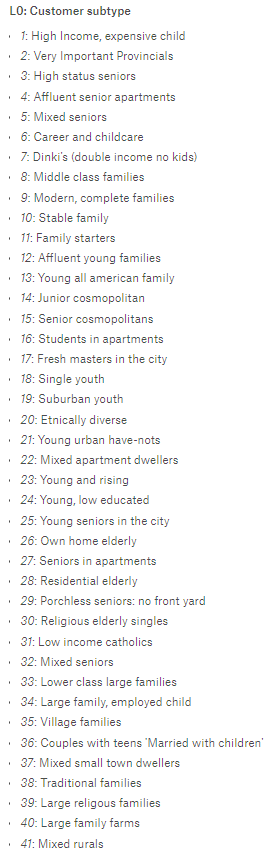
\includegraphics{images/customersubtype.png}
\end{figure}
A key for average age:
\begin{figure}[H]
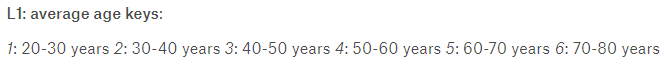
\includegraphics{images/averageage.png}
\end{figure}
A key of customer main types:
\begin{figure}[H]
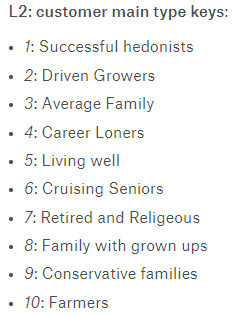
\includegraphics{images/customermaintype.png}
\end{figure}
A key of percentage ranges:
\begin{figure}[H]
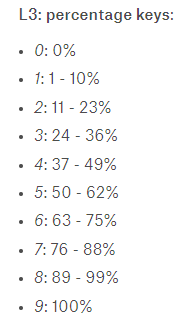
\includegraphics{images/percentage.png}
\end{figure}
and a key of total number ranges:
\begin{figure}[H]
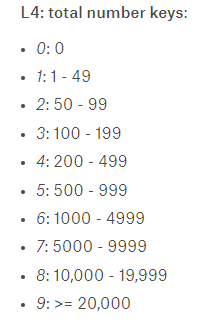
\includegraphics{images/totalnumber.png}
\end{figure}
I will use these keys to turn the appropriate columns into factors later, by maping the numeric values in the dataset to the appropritae value from the keys. 

I will now take a look at the class label distribution
\begin{knitrout}
\definecolor{shadecolor}{rgb}{0.969, 0.969, 0.969}\color{fgcolor}\begin{kframe}
\begin{alltt}
\hlcom{#Class label freq}
\hlstd{classLabelFreq} \hlkwb{<-} \hlkwd{data.frame}\hlstd{(df}\hlopt{$}\hlstd{CARAVAN)}
\hlstd{classLabelFreq}\hlopt{$}\hlstd{df.CARAVAN} \hlkwb{<-} \hlkwd{as.factor}\hlstd{(df}\hlopt{$}\hlstd{CARAVAN)}

\hlcom{#Class label Distribution Plot }
\hlkwd{ggplot}\hlstd{(classLabelFreq,}\hlkwd{aes}\hlstd{(}\hlkwc{x}\hlstd{=df.CARAVAN))} \hlopt{+} \hlkwd{geom_bar}\hlstd{()} \hlopt{+} \hlkwd{labs}\hlstd{(}\hlkwc{x}\hlstd{=}\hlstr{"CARAVAN"}\hlstd{)}
\end{alltt}
\end{kframe}
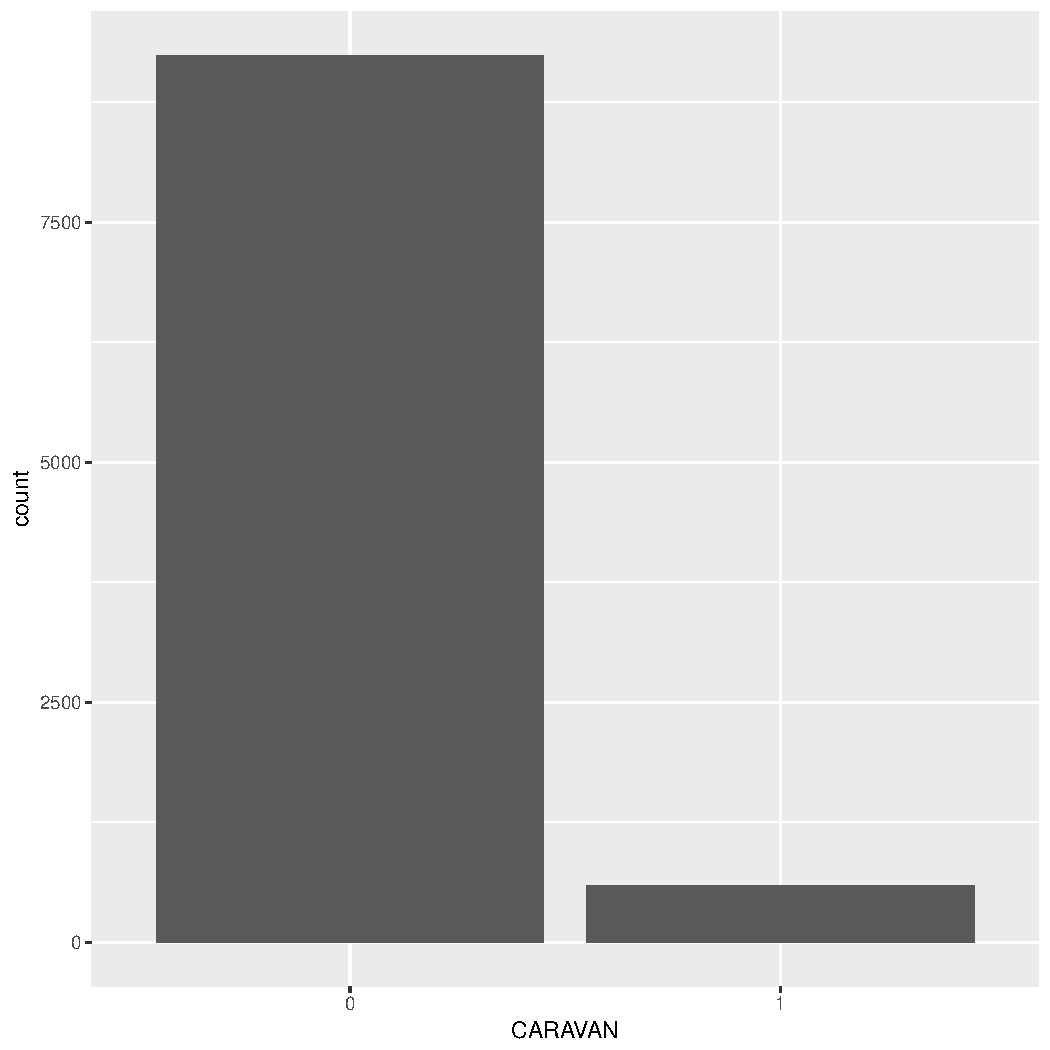
\includegraphics[width=\maxwidth]{figure/unnamed-chunk-6-1} 
\begin{kframe}\begin{alltt}
\hlcom{#Size of each factor level }
\hlkwd{length}\hlstd{(classLabelFreq[classLabelFreq}\hlopt{$}\hlstd{df.CARAVAN}\hlopt{==}\hlstr{"0"}\hlstd{,])}
\end{alltt}
\begin{verbatim}
## [1] 9236
\end{verbatim}
\begin{alltt}
\hlkwd{length}\hlstd{(classLabelFreq[classLabelFreq}\hlopt{$}\hlstd{df.CARAVAN}\hlopt{==}\hlstr{"1"}\hlstd{,])}
\end{alltt}
\begin{verbatim}
## [1] 586
\end{verbatim}
\end{kframe}
\end{knitrout}

There are 586 records that are likely to want caravan insurance. 9236 records that do not. Dataset has an imbalanced distribution in the class label. I will use a resampling technique during pre-processing to compensate for this. 

Lets take a look at the disribution of Main Customer Type
\begin{knitrout}
\definecolor{shadecolor}{rgb}{0.969, 0.969, 0.969}\color{fgcolor}\begin{kframe}
\begin{alltt}
\hlcom{#Cust main type}
\hlstd{custMainType} \hlkwb{<-} \hlkwd{data.frame}\hlstd{(df}\hlopt{$}\hlstd{MOSHOOFD,df}\hlopt{$}\hlstd{CARAVAN)}
\hlstd{custMainType}\hlopt{$}\hlstd{df.MOSHOOFD} \hlkwb{<-} \hlkwd{as.factor}\hlstd{(custMainType}\hlopt{$}\hlstd{df.MOSHOOFD)}
\hlstd{custMainType}\hlopt{$}\hlstd{df.CARAVAN} \hlkwb{<-} \hlkwd{as.factor}\hlstd{(custMainType}\hlopt{$}\hlstd{df.CARAVAN)}

\hlcom{#Plot of Customer Main Type}
\hlstd{plot}\hlkwb{<-}\hlkwd{ggplot}\hlstd{(custMainType,}\hlkwd{aes}\hlstd{(}\hlkwc{x}\hlstd{=}\hlkwd{reorder}\hlstd{(df.MOSHOOFD,df.MOSHOOFD,}\hlkwa{function}\hlstd{(}\hlkwc{x}\hlstd{)}\hlopt{-}\hlkwd{length}\hlstd{(x)),}\hlkwc{fill}\hlstd{=df.CARAVAN))}
\hlstd{plot}\hlkwb{<-}\hlstd{plot} \hlopt{+} \hlkwd{geom_bar}\hlstd{()}
\hlstd{plot}\hlkwb{<-}\hlstd{plot} \hlopt{+} \hlkwd{labs}\hlstd{(}\hlkwc{x}\hlstd{=}\hlstr{"Customer Main Type"}\hlstd{)}
\hlstd{plot}
\end{alltt}
\end{kframe}
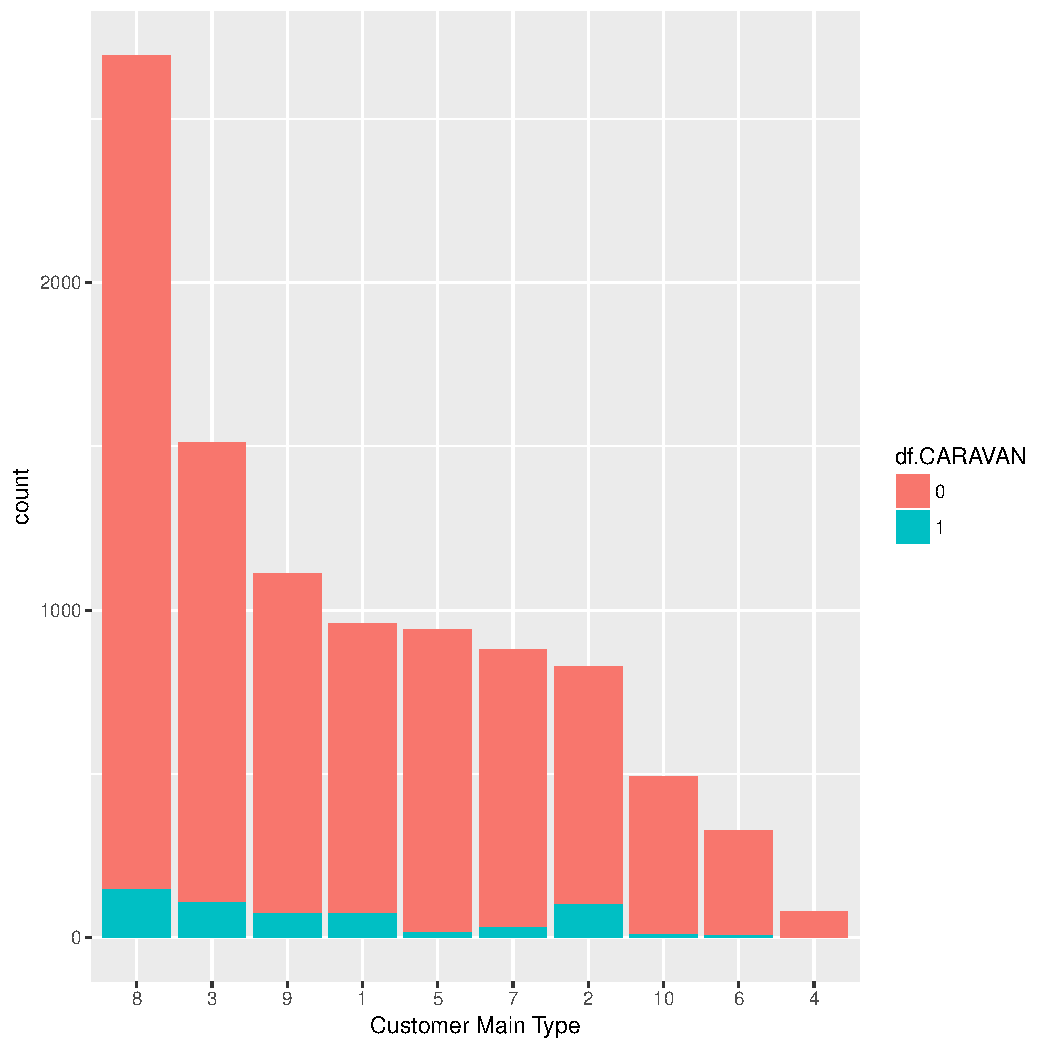
\includegraphics[width=\maxwidth]{figure/unnamed-chunk-7-1} 

\end{knitrout}

Most frequent Main Customer Type is 8:Family with Grown Ups, 2nd Most frequent is 3:Average Family and the 3rd most frequent is 9:conservative families. 

The least frequent type is 4:Career Loners ,2nd least frequent is 6:Cruising Seniors and the 3rd least frequent is 10:Farmers. 

Comparing to where CARAVAN is TRUE, you can see that the two most frequent main types are the same as the whole dataset. Customer Main Type 2: Driven Growers seems to be a bit more prominent where CARAVAN is true. You can also see that there are no instances of group 4: Career Loners in the rows where CARAVAN is true. 

Lets take a closer look at the rows where CARAVAN is TRUE:
\begin{knitrout}
\definecolor{shadecolor}{rgb}{0.969, 0.969, 0.969}\color{fgcolor}\begin{kframe}
\begin{alltt}
\hlcom{#Wants caravan }
\hlstd{wantsCaravan} \hlkwb{<-} \hlstd{df[df}\hlopt{$}\hlstd{CARAVAN}\hlopt{==}\hlnum{1}\hlstd{,]}
\hlstd{wantsCaravan}\hlopt{$}\hlstd{MOSHOOFD} \hlkwb{<-} \hlkwd{as.factor}\hlstd{(wantsCaravan}\hlopt{$}\hlstd{MOSHOOFD)}
\hlstd{wantsCaravan}\hlopt{$}\hlstd{MOSTYPE} \hlkwb{<-} \hlkwd{as.factor}\hlstd{(wantsCaravan}\hlopt{$}\hlstd{MOSTYPE)}

\hlcom{#Plot of Customer Main Type where wants caravan}
\hlstd{plot}\hlkwb{<-}\hlkwd{ggplot}\hlstd{(wantsCaravan,}\hlkwd{aes}\hlstd{(}\hlkwc{x}\hlstd{=}\hlkwd{reorder}\hlstd{(MOSHOOFD,MOSHOOFD,}\hlkwa{function}\hlstd{(}\hlkwc{x}\hlstd{)}\hlopt{-}\hlkwd{length}\hlstd{(x))))}
\hlstd{plot}\hlkwb{<-}\hlstd{plot} \hlopt{+} \hlkwd{geom_bar}\hlstd{()}
\hlstd{plot}\hlkwb{<-}\hlstd{plot} \hlopt{+} \hlkwd{labs}\hlstd{(}\hlkwc{x}\hlstd{=}\hlstr{"Customer Main Type"}\hlstd{)}
\hlstd{plot}
\end{alltt}
\end{kframe}
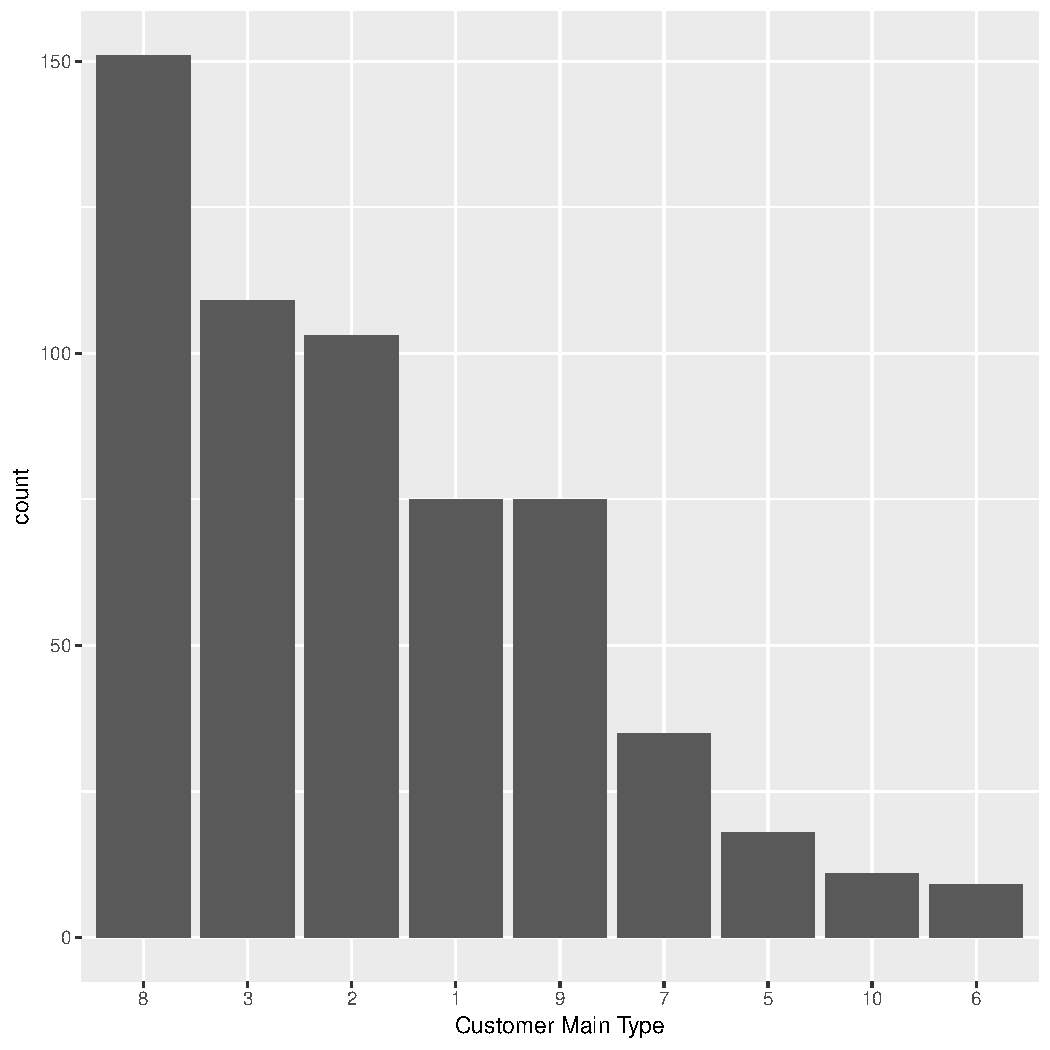
\includegraphics[width=\maxwidth]{figure/unnamed-chunk-8-1} 
\begin{kframe}\begin{alltt}
\hlcom{#Max and Min}
\hlstd{mainCustType} \hlkwb{=} \hlkwd{table}\hlstd{(wantsCaravan}\hlopt{$}\hlstd{MOSHOOFD)}
\hlkwd{names}\hlstd{(}\hlkwd{which.max}\hlstd{(mainCustType))}
\end{alltt}
\begin{verbatim}
## [1] "8"
\end{verbatim}
\begin{alltt}
\hlkwd{names}\hlstd{(}\hlkwd{which.min}\hlstd{(mainCustType))}
\end{alltt}
\begin{verbatim}
## [1] "6"
\end{verbatim}
\end{kframe}
\end{knitrout}

The top 3 Main Customer Types are 8:Family with Grown Ups, 3: Average Family and 2:Driven Growers. As stated before the first 2 types are the same as the dataset as a whole. Type 2:Driven Growers has now overtaken 9:conservative families. 9:Conservative Families is joint 4th. Interesting that category 1: Successful Hedonists has the same number of occurances as 9:Conservaite Families. Hedonists are people who devote their lives to the pursuit of pleasure. There is perhaps a connection there between the idea of traveling by caravan and being a hedonist. 

The 3 least frequent Main Custom Types 6:Cruising Seniors ,10:Farmers and 5:Living Well. As stated before there are no instances of 4:Career Loners when CARAVAN is TRUE. There is too small a number of instances of 4:Career Loners in the whole dataset to really say there is correlation but it is possible. 

Now going to take a look at Customer Subtype
\begin{knitrout}
\definecolor{shadecolor}{rgb}{0.969, 0.969, 0.969}\color{fgcolor}\begin{kframe}
\begin{alltt}
\hlcom{#Sub cust type}
\hlstd{subCustType} \hlkwb{<-} \hlkwd{data.frame}\hlstd{(df}\hlopt{$}\hlstd{MOSTYPE,df}\hlopt{$}\hlstd{CARAVAN)}
\hlstd{subCustType}\hlopt{$}\hlstd{df.MOSTYPE} \hlkwb{<-} \hlkwd{as.factor}\hlstd{(subCustType}\hlopt{$}\hlstd{df.MOSTYPE)}
\hlstd{subCustType}\hlopt{$}\hlstd{df.CARAVAN} \hlkwb{<-} \hlkwd{as.factor}\hlstd{(subCustType}\hlopt{$}\hlstd{df.CARAVAN)}

\hlcom{#Plot of Customer subtype}
\hlstd{plot}\hlkwb{<-}\hlkwd{ggplot}\hlstd{(subCustType,}\hlkwd{aes}\hlstd{(}\hlkwc{x}\hlstd{=}\hlkwd{reorder}\hlstd{(df.MOSTYPE,df.MOSTYPE,}\hlkwa{function}\hlstd{(}\hlkwc{x}\hlstd{)}\hlopt{-}\hlkwd{length}\hlstd{(x)),}\hlkwc{fill}\hlstd{=df.CARAVAN))}
\hlstd{plot}\hlkwb{<-}\hlstd{plot} \hlopt{+} \hlkwd{geom_bar}\hlstd{()}
\hlstd{plot}\hlkwb{<-}\hlstd{plot} \hlopt{+} \hlkwd{labs}\hlstd{(}\hlkwc{x}\hlstd{=}\hlstr{"Customer Subtype"}\hlstd{)}
\hlstd{plot}
\end{alltt}
\end{kframe}
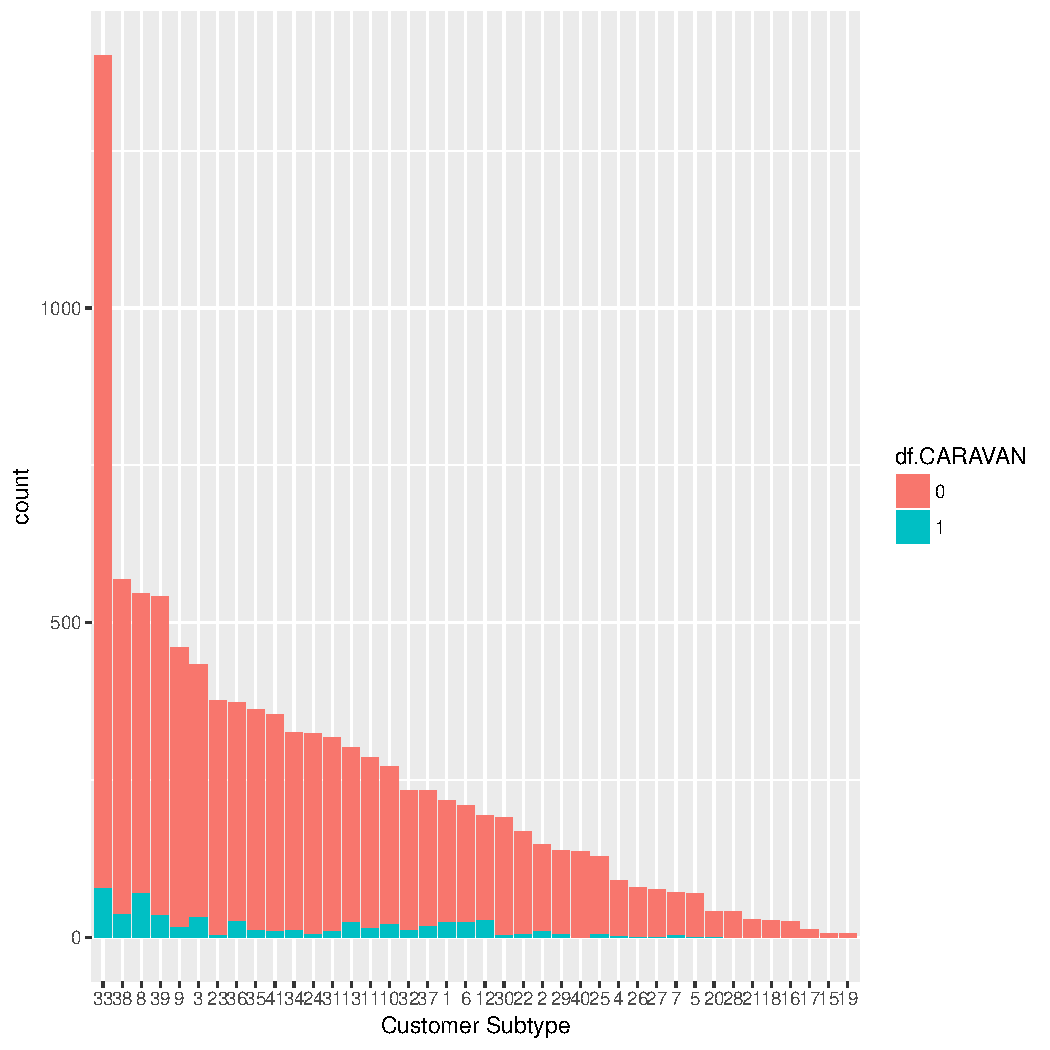
\includegraphics[width=\maxwidth]{figure/unnamed-chunk-9-1} 

\end{knitrout}
The top 3 subtypes are 33:Lower class large families ,38:Traditional families  and 8:Middle class families. 

The bottom 3 are 19:Suburban Youth ,15:Senior cosmopolitans and 17:Fresh masters in the city. The dataset contains mostly data about families. 

Taking a look at when CARAVAN is TRUE, you can see that It doesn't follow the same trend in frequency as the dataset as a whole This might mean that It could be used as a useful predictor. You can also see that there are no rows where CARAVAN is true that have subtypes of 40:Large family farms, 21:Young urban have-nots, 18:Single youth, 16:Students in apartments, 17:Fresh masters in the city, 15:Senior cosmopolitans and 19:Suburban youth. 

This could suggest that postcode areas most comprised with familes are more likely to purchase caravan insurance. 

Going to take a look at customer subtype when CARAVAN is TRUE
\begin{knitrout}
\definecolor{shadecolor}{rgb}{0.969, 0.969, 0.969}\color{fgcolor}\begin{kframe}
\begin{alltt}
\hlcom{#Plot of Customer Subtype where wants caravan }
\hlstd{plot}\hlkwb{<-}\hlkwd{ggplot}\hlstd{(wantsCaravan,}\hlkwd{aes}\hlstd{(}\hlkwc{x}\hlstd{=}\hlkwd{reorder}\hlstd{(MOSTYPE,MOSTYPE,}\hlkwa{function}\hlstd{(}\hlkwc{x}\hlstd{)}\hlopt{-}\hlkwd{length}\hlstd{(x))))}
\hlstd{plot}\hlkwb{<-}\hlstd{plot} \hlopt{+} \hlkwd{geom_bar}\hlstd{()}
\hlstd{plot}\hlkwb{<-}\hlstd{plot} \hlopt{+} \hlkwd{labs}\hlstd{(}\hlkwc{x}\hlstd{=}\hlstr{"Customer Subtype"}\hlstd{)}
\hlstd{plot}
\end{alltt}
\end{kframe}
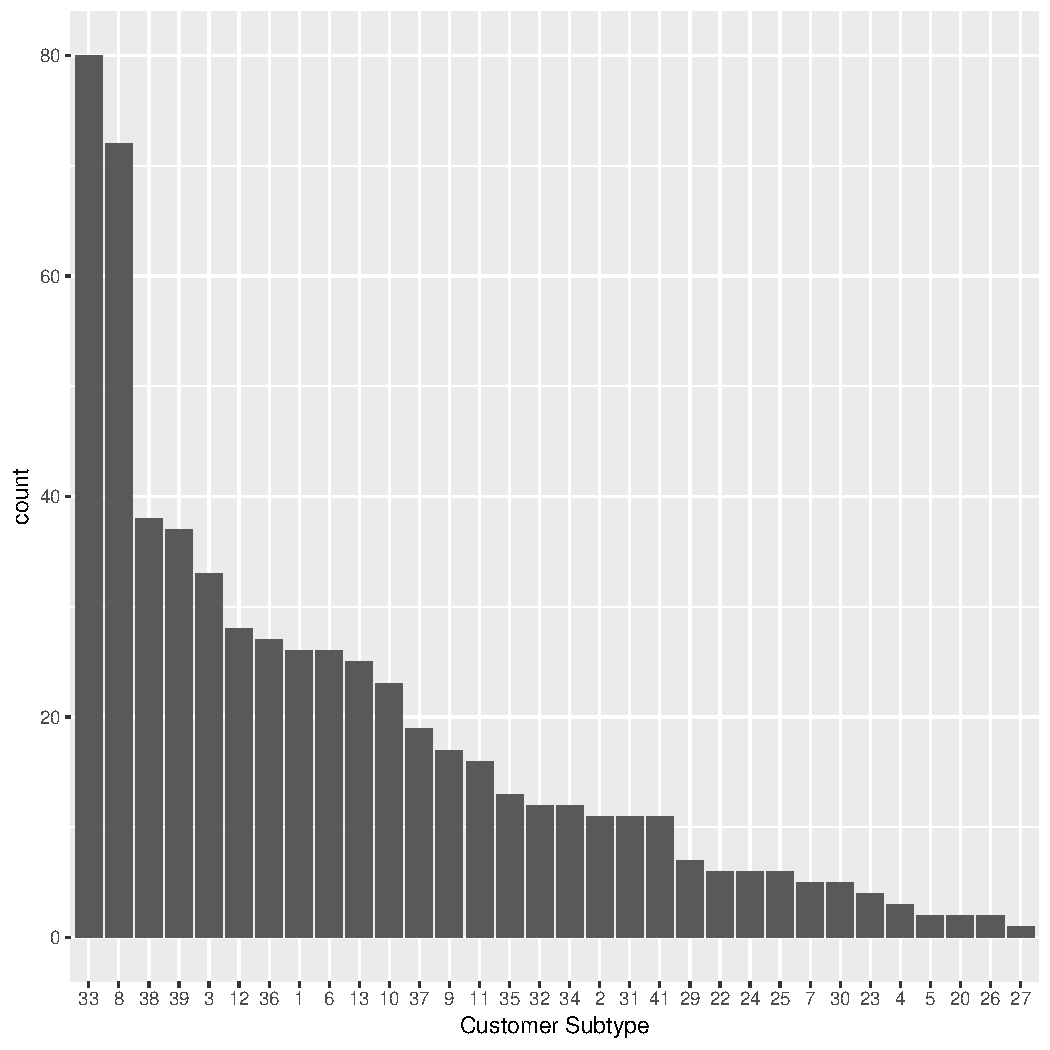
\includegraphics[width=\maxwidth]{figure/unnamed-chunk-10-1} 
\begin{kframe}\begin{alltt}
\hlcom{#Max and Min }
\hlstd{subCustType} \hlkwb{=} \hlkwd{table}\hlstd{(wantsCaravan}\hlopt{$}\hlstd{MOSTYPE)}
\hlkwd{names}\hlstd{(}\hlkwd{which.max}\hlstd{(subCustType))}
\end{alltt}
\begin{verbatim}
## [1] "33"
\end{verbatim}
\begin{alltt}
\hlkwd{names}\hlstd{(}\hlkwd{which.min}\hlstd{(subCustType))}
\end{alltt}
\begin{verbatim}
## [1] "27"
\end{verbatim}
\end{kframe}
\end{knitrout}
Top 3 subtypes are the same as the datset as a whole but subtype 8:Middle class families is now more frequent than 38:Traditional families. This might mean that areas consisting of lower to middle class families are more likely to purchase caravan insurance than areas with mostly traditional families. 

The bottom 3 subtypes are 27:Seniors in apartments ,26:Own home elderly and 20:Ethnically diverse. This supports the theory that areas with higher amounts of families are the most likely to purchase caravan insurance. 

I am not going to take a look at two columns. MAANTHUI(Number of houses) and MGEMOMV(Avg size of household). MAATHUI is in the range of 1-10 and MGEMOMV is in the range of 1-6. They are the only two numeric values in the dataset the rest are factors. I will look at them together to see if there is any corelation. I will use ggplot2 again to make a scatter plot. These are integer values there will be overlap. 

\begin{knitrout}
\definecolor{shadecolor}{rgb}{0.969, 0.969, 0.969}\color{fgcolor}\begin{kframe}
\begin{alltt}
\hlcom{#Number of Houses and Avg size of household}
\hlstd{houseData}\hlkwb{<-}\hlkwd{data.frame}\hlstd{(df}\hlopt{$}\hlstd{MAANTHUI,df}\hlopt{$}\hlstd{MGEMOMV,df}\hlopt{$}\hlstd{CARAVAN)}
\hlstd{houseData}\hlopt{$}\hlstd{df.CARAVAN}\hlkwb{<-}\hlkwd{as.factor}\hlstd{(houseData}\hlopt{$}\hlstd{df.CARAVAN)}

\hlcom{#ScatterPlot of both}
\hlstd{plot}\hlkwb{<-}\hlkwd{ggplot}\hlstd{(houseData,}\hlkwd{aes}\hlstd{(}\hlkwc{x}\hlstd{=df.MAANTHUI,}\hlkwc{y}\hlstd{=df.MGEMOMV))}
\hlstd{plot}\hlkwb{<-}\hlstd{plot} \hlopt{+} \hlkwd{geom_point}\hlstd{(}\hlkwd{aes}\hlstd{(}\hlkwc{shape}\hlstd{=df.CARAVAN))}
\hlstd{plot}\hlkwb{<-}\hlstd{plot} \hlopt{+} \hlkwd{scale_shape}\hlstd{(}\hlkwc{solid}\hlstd{=}\hlnum{FALSE}\hlstd{)}
\hlstd{plot}\hlkwb{<-}\hlstd{plot} \hlopt{+} \hlkwd{labs}\hlstd{(}\hlkwc{x}\hlstd{=}\hlstr{"Number of Houses"}\hlstd{,} \hlkwc{y}\hlstd{=}\hlstr{"Average Household Size"}\hlstd{)}
\hlstd{plot}
\end{alltt}
\end{kframe}
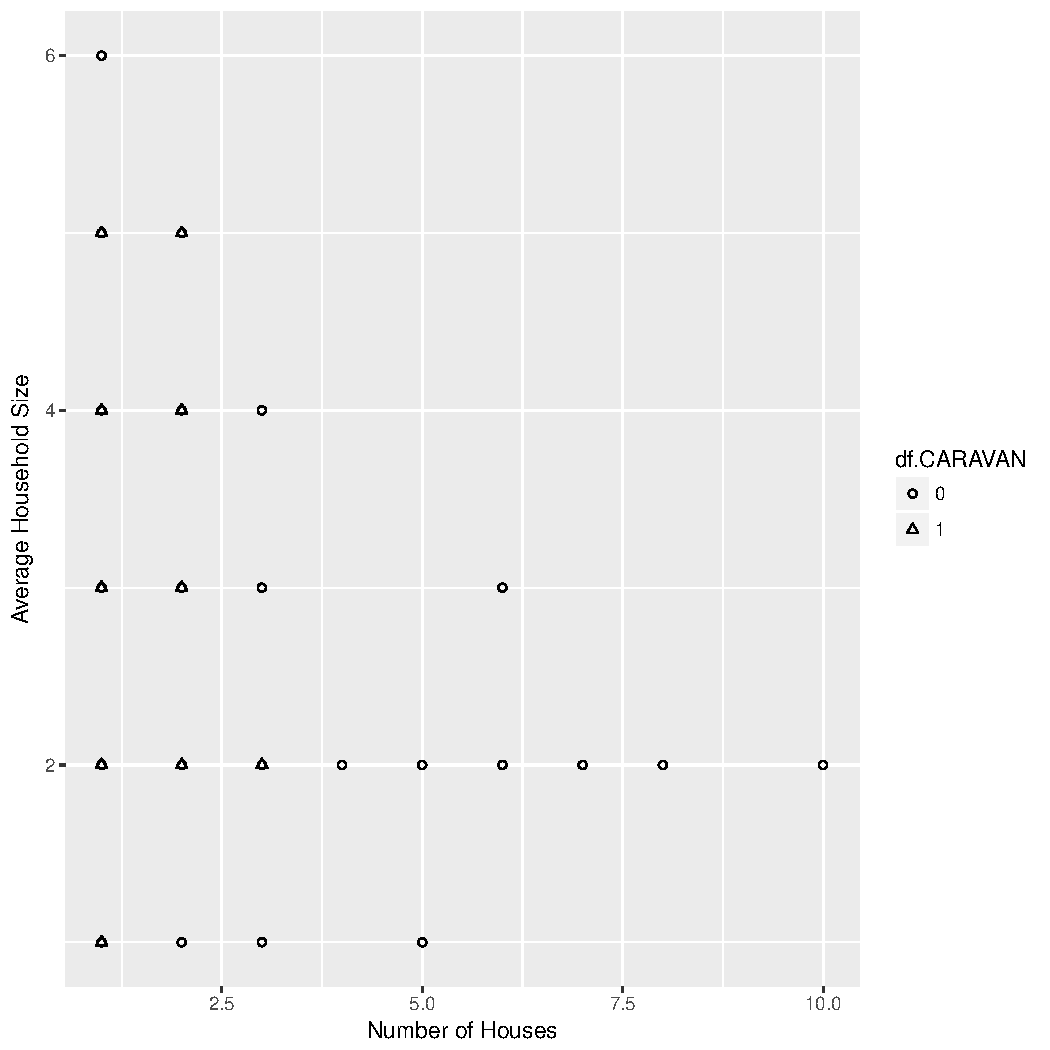
\includegraphics[width=\maxwidth]{figure/unnamed-chunk-11-1} 

\end{knitrout}
Taking a look at the results, average size of household decreases as the number of houses increases which makes sense. Looking at the points where CARAVAN is TRUE, There are no points when the number of houses is greater than 3. There are also no points when the average house size is greater than 5. This shows a potential connection between number of houses and CARAVAN. If I had to remove one of the two variables I would remove Average house size as I think number of houses has a greater corelation to CARAVAN equaling TRUE

I will now take a look at the average age variable, MGEMLEEF. 
\begin{knitrout}
\definecolor{shadecolor}{rgb}{0.969, 0.969, 0.969}\color{fgcolor}\begin{kframe}
\begin{alltt}
\hlcom{#Average Age }
\hlstd{averageAge} \hlkwb{<-} \hlkwd{data.frame}\hlstd{(df}\hlopt{$}\hlstd{MGEMLEEF,df}\hlopt{$}\hlstd{CARAVAN)}
\hlstd{averageAge}\hlopt{$}\hlstd{df.MGEMLEEF} \hlkwb{<-} \hlkwd{as.factor}\hlstd{(averageAge}\hlopt{$}\hlstd{df.MGEMLEEF)}
\hlstd{averageAge}\hlopt{$}\hlstd{df.CARAVAN} \hlkwb{<-} \hlkwd{as.factor}\hlstd{(averageAge}\hlopt{$}\hlstd{df.CARAVAN)}

\hlcom{#Plot of Average Age }
\hlstd{plot}\hlkwb{<-}\hlkwd{ggplot}\hlstd{(averageAge,}\hlkwd{aes}\hlstd{(}\hlkwc{x}\hlstd{=df.MGEMLEEF,}\hlkwc{fill}\hlstd{=df.CARAVAN))}
\hlstd{plot}\hlkwb{<-}\hlstd{plot} \hlopt{+} \hlkwd{geom_bar}\hlstd{()}
\hlstd{plot}\hlkwb{<-}\hlstd{plot} \hlopt{+} \hlkwd{labs}\hlstd{(}\hlkwc{x}\hlstd{=}\hlstr{"Average Age"}\hlstd{)}
\hlstd{plot}
\end{alltt}
\end{kframe}
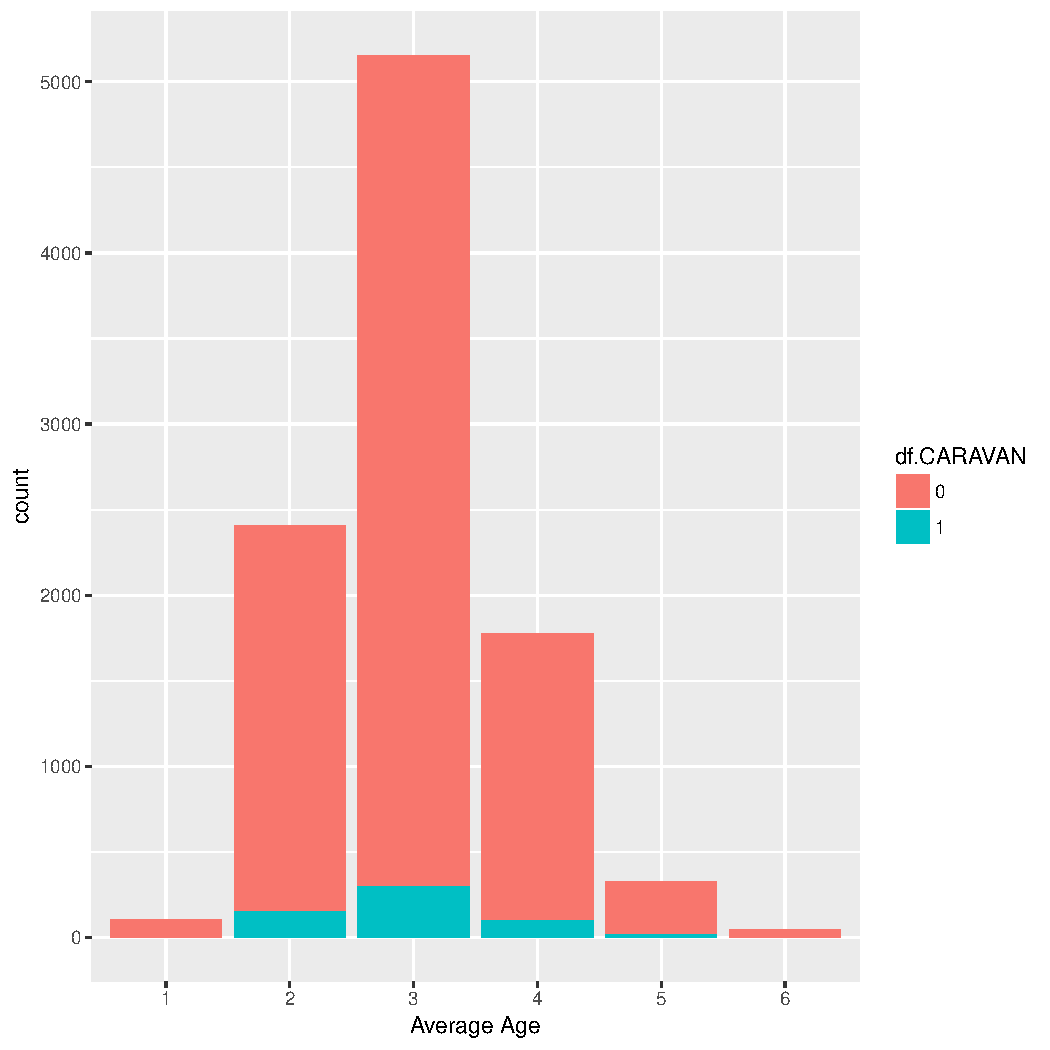
\includegraphics[width=\maxwidth]{figure/unnamed-chunk-12-1} 

\end{knitrout}
Average age is a factor, where each level is a range of ages. Lowest age range is 1:20-30 years, highest is 6:70-80 years. Looking at the graph, levels 3:40-50, 2:30-40 and 4:50-60 are the top 3 most frequent values. The extremes of 1 and 6 are the two lowest and do not have very many occurances. Looking at instances where CARAVAN is TRUE, They are in the same order as the whole dataset. Except there are no instances where CARAVAN is TRUE that contain 1 and 6 for average age.There might be a trend that areas were the average age is 1:20-30 or 6:70-80 would not buy caravan insurance. There isn't enough data to be sure and as the data where CARAVAN is true follows a similar trend to the data as a whole its unlikely there is a corelation between average age and CARAVAN. 

The first column in the data set is ORIGIN. It has two values
\begin{knitrout}
\definecolor{shadecolor}{rgb}{0.969, 0.969, 0.969}\color{fgcolor}\begin{kframe}
\begin{alltt}
\hlcom{#Levels of ORIGIN}
\hlkwd{levels}\hlstd{(df}\hlopt{$}\hlstd{ORIGIN)}
\end{alltt}
\begin{verbatim}
## [1] "test"  "train"
\end{verbatim}
\end{kframe}
\end{knitrout}
This is the original source of the row from the challenge. The rows are already split into a train set and test set. I will remove this column later during pre-processing, as I plan to resample the data and split the data into train and test sets myself. 

I have noW looked at all the main variables. 

I am not going to take a look at the APERSAUT column, which is the Number of Car Policies column. This is a factor, where each level equates to a range of values. The ranges are defined in the total number key. I have a feeling that it might be an important predictor, so want to try and confirm my theory.  
\begin{knitrout}
\definecolor{shadecolor}{rgb}{0.969, 0.969, 0.969}\color{fgcolor}\begin{kframe}
\begin{alltt}
\hlcom{#Number of Car Policies}
\hlstd{numberOfCarPolicies} \hlkwb{<-} \hlkwd{data.frame}\hlstd{(df}\hlopt{$}\hlstd{APERSAUT,df}\hlopt{$}\hlstd{CARAVAN)}
\hlstd{numberOfCarPolicies}\hlopt{$}\hlstd{df.APERSAUT} \hlkwb{<-} \hlkwd{as.factor}\hlstd{(numberOfCarPolicies}\hlopt{$}\hlstd{df.APERSAUT)}
\hlstd{numberOfCarPolicies}\hlopt{$}\hlstd{df.CARAVAN} \hlkwb{<-} \hlkwd{as.factor}\hlstd{(numberOfCarPolicies}\hlopt{$}\hlstd{df.CARAVAN)}

\hlcom{#Plot of APERSAUT}
\hlstd{plot}\hlkwb{<-}\hlkwd{ggplot}\hlstd{(numberOfCarPolicies,}\hlkwd{aes}\hlstd{(}\hlkwc{x}\hlstd{=}\hlkwd{reorder}\hlstd{(df.APERSAUT,df.APERSAUT,}\hlkwa{function}\hlstd{(}\hlkwc{x}\hlstd{)}\hlopt{-}\hlkwd{length}\hlstd{(x)),}\hlkwc{fill}\hlstd{=df.CARAVAN))}
\hlstd{plot}\hlkwb{<-}\hlstd{plot} \hlopt{+} \hlkwd{geom_bar}\hlstd{()}
\hlstd{plot}\hlkwb{<-}\hlstd{plot} \hlopt{+} \hlkwd{labs}\hlstd{(}\hlkwc{x}\hlstd{=}\hlstr{"Number of Car Policies"}\hlstd{)}
\hlstd{plot}
\end{alltt}
\end{kframe}
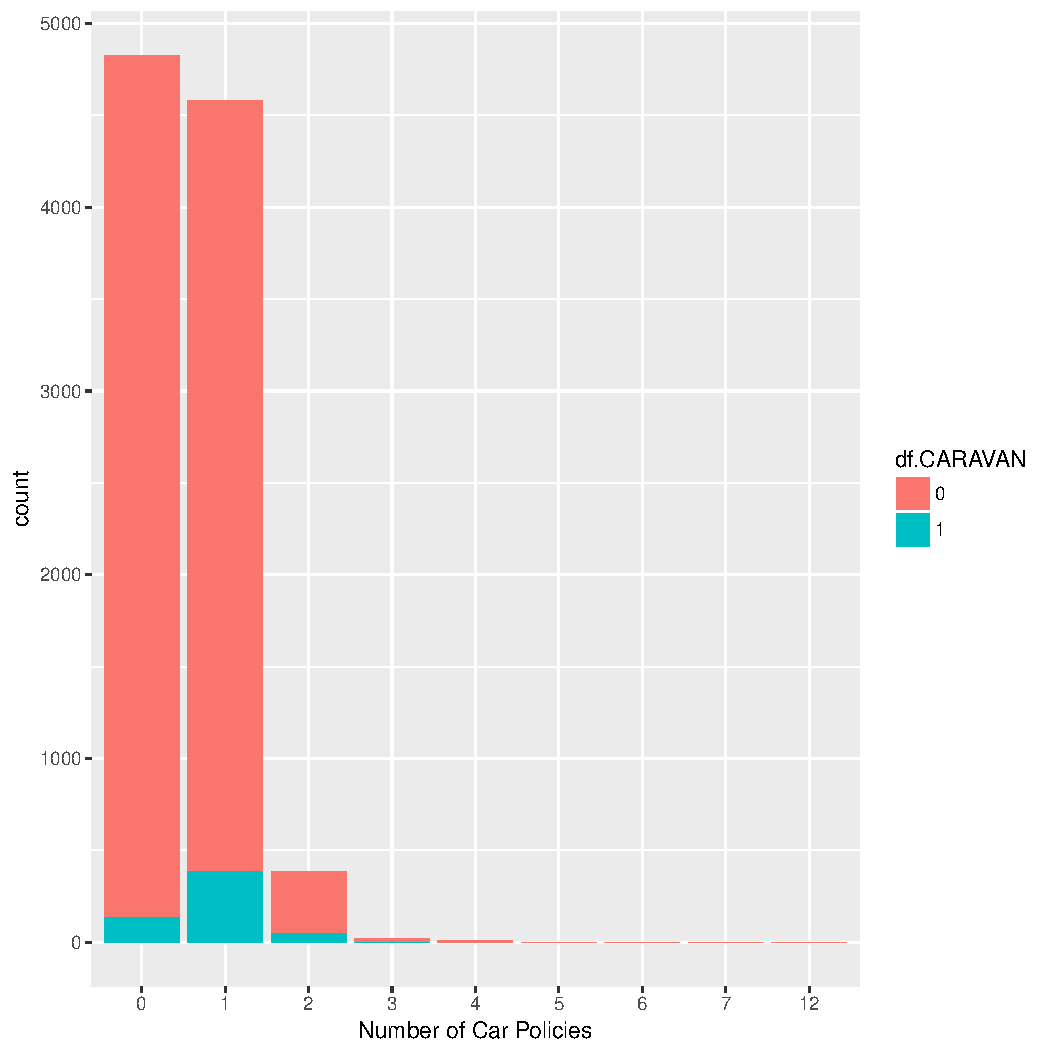
\includegraphics[width=\maxwidth]{figure/unnamed-chunk-14-1} 

\end{knitrout}
There is a factor level of 12 here on the graph. There is only supposed to be levels 0-9. This is likely a mistake in the dataset. When I factor this column later during pre processing and remove n/a values this wrong value should get removed. 

Looking at when CARAVAN is TRUE, there is a possible relation between when the number of car policies are the level 1:1-49 and when CARAVAN is TRUE. 
\begin{knitrout}
\definecolor{shadecolor}{rgb}{0.969, 0.969, 0.969}\color{fgcolor}\begin{kframe}
\begin{alltt}
\hlcom{#Number of Car Policies When Caravan is TRUE}
\hlstd{wantsCaravan}\hlopt{$}\hlstd{APERSAUT} \hlkwb{<-} \hlkwd{as.factor}\hlstd{(wantsCaravan}\hlopt{$}\hlstd{APERSAUT)}

\hlcom{#Plot of number of car policies (caravan is TRUE)}
\hlstd{plot}\hlkwb{<-}\hlkwd{ggplot}\hlstd{(wantsCaravan,}\hlkwd{aes}\hlstd{(}\hlkwc{x}\hlstd{=APERSAUT))}
\hlstd{plot}\hlkwb{<-}\hlstd{plot} \hlopt{+} \hlkwd{geom_bar}\hlstd{()}
\hlstd{plot}\hlkwb{<-}\hlstd{plot} \hlopt{+} \hlkwd{labs}\hlstd{(}\hlkwc{x}\hlstd{=}\hlstr{"Number of Car Policies"}\hlstd{)}
\hlstd{plot}
\end{alltt}
\end{kframe}
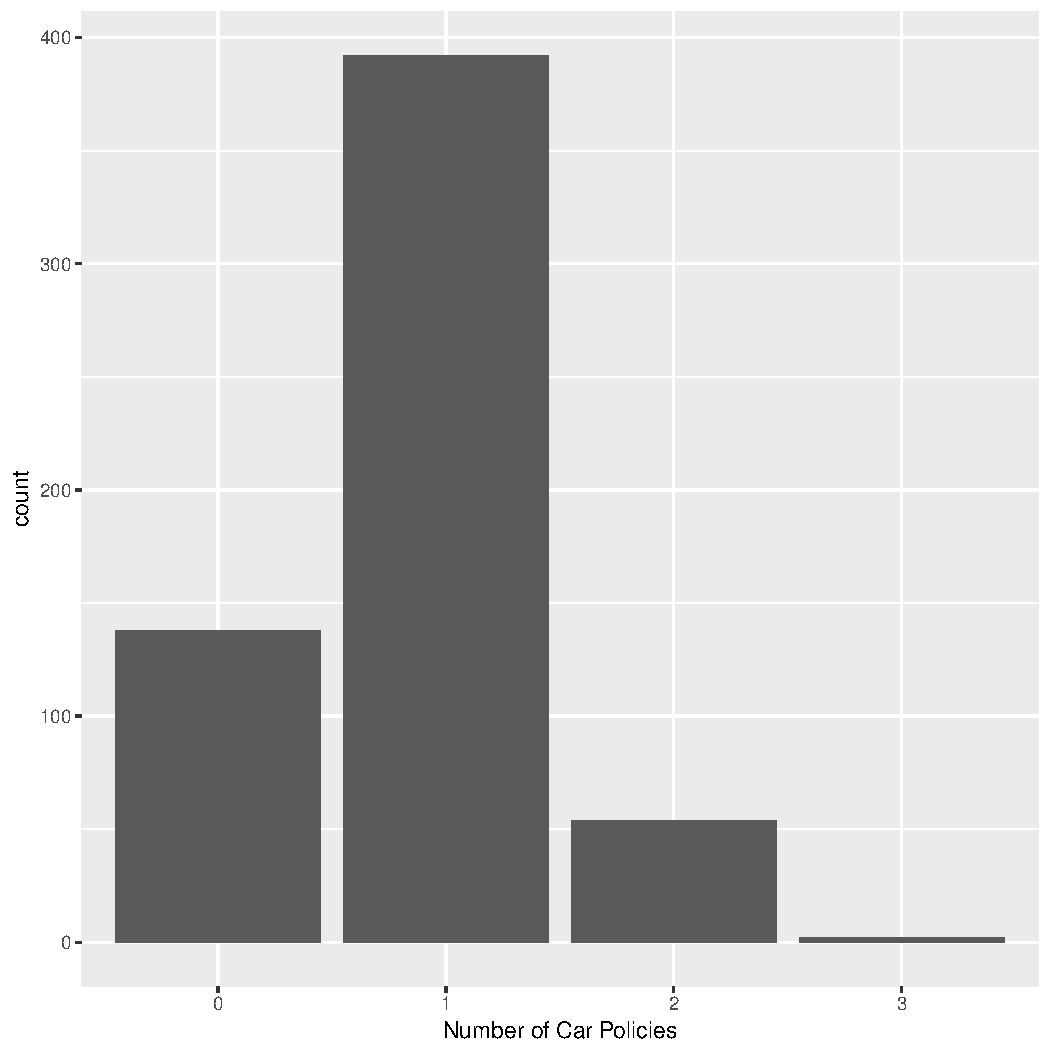
\includegraphics[width=\maxwidth]{figure/unnamed-chunk-15-1} 

\end{knitrout}
This factor is supposed to have 9 levels in total, but this column factored only contains the lowest 4 possible factors, 0,1,2 and 3. 1 is the most frequent. In this case 1 represents the range of values 1-49. 0 represents 0, 2 represents the range of values 50-99 and 3 represents the range of values 100-199. 

This would suggest that post codes that contain a number of cars in the range of 1-49 are most likey to purchase caravan insurance. There are only 2 rows in the dataset that contain 3 for this column so this could be considered an outlier. Based on the graph the range of values for number of cars could be 0-99, or 0-199 if you include the two rows that have the value 3. There isn't enough data here to be sure. 

I was originally confused by this result. I had assumed that I would find the opposite, that areas with large numbers of cars would likey need caravan insurance as I assumed you would need a car to tow a caravan. After further study of the information about the dataset, in this case CARAVAN actually refers to mobile homes. This would suggest the data is based on american post codes (or area codes) and that 'caravan' refers to a self driving vehicle that you can sleep in rather than a traditional british caravan. 

Based on the graph its possible there is a correlation between this variable and CARAVAN being TRUE. This variable might be an important predictor. 

\subsection{Pre-Proccessing}
I will now pre-process my data before I begin building models

First I will rename all the columns. This will make them a little easier to understand, and means I do not have to keep refering to the keys. I will use the dplyr package to do this.
\begin{knitrout}
\definecolor{shadecolor}{rgb}{0.969, 0.969, 0.969}\color{fgcolor}\begin{kframe}
\begin{alltt}
\hlkwd{library}\hlstd{(dplyr)}
\end{alltt}


{\ttfamily\noindent\color{warningcolor}{\#\# Warning: package 'dplyr' was built under R version 3.4.2}}

{\ttfamily\noindent\itshape\color{messagecolor}{\#\# \\\#\# Attaching package: 'dplyr'}}

{\ttfamily\noindent\itshape\color{messagecolor}{\#\# The following objects are masked from 'package:stats':\\\#\# \\\#\#\ \ \ \  filter, lag}}

{\ttfamily\noindent\itshape\color{messagecolor}{\#\# The following objects are masked from 'package:base':\\\#\# \\\#\#\ \ \ \  intersect, setdiff, setequal, union}}\end{kframe}
\end{knitrout}
This is a package used for manipulating frame objects in r. I will now use the rename function to rename the columns
\begin{knitrout}
\definecolor{shadecolor}{rgb}{0.969, 0.969, 0.969}\color{fgcolor}\begin{kframe}
\begin{alltt}
\hlcom{#Rename columns }
\hlstd{df}\hlkwb{<-}\hlkwd{rename}\hlstd{(df,}\hlkwc{Customer_Subtype}\hlstd{=MOSTYPE,}
           \hlkwc{Number_of_Houses}\hlstd{=MAANTHUI,}
           \hlkwc{Avg_Size_Household}\hlstd{=MGEMOMV,}
           \hlkwc{Avg_Age}\hlstd{=MGEMLEEF,}
           \hlkwc{Customer_Main_Type}\hlstd{=MOSHOOFD,}
           \hlkwc{Percentage_Roman_Catholic}\hlstd{=MGODRK,}
           \hlkwc{Percentage_Protestant}\hlstd{=MGODPR,}
           \hlkwc{Percentage_Other_Religion}\hlstd{=MGODOV,}
           \hlkwc{Percentage_No_Religion}\hlstd{=MGODGE,}
           \hlkwc{Percentage_Married}\hlstd{=MRELGE,}
           \hlkwc{Percentage_Living_Together}\hlstd{=MRELSA,}
           \hlkwc{Percentage_Other_Relation}\hlstd{=MRELOV,}
           \hlkwc{Percentage_Singles}\hlstd{=MFALLEEN,}
           \hlkwc{Percentage_Household_without_Children}\hlstd{=MFGEKIND,}
           \hlkwc{Percentage_Household_with_Children}\hlstd{=MFWEKIND,}
           \hlkwc{Percentage_High_Level_Education}\hlstd{=MOPLHOOG,}
           \hlkwc{Percentage_Middle_Level_Education}\hlstd{=MOPLMIDD,}
           \hlkwc{Percentage_Low_Level_Education}\hlstd{=MOPLLAAG,}
           \hlkwc{Percentage_High_Status}\hlstd{=MBERHOOG,}
           \hlkwc{Percentage_Entrepreneur}\hlstd{=MBERZELF,}
           \hlkwc{Percentage_Farmer}\hlstd{=MBERBOER,}
           \hlkwc{Percentage_Middle_Management}\hlstd{=MBERMIDD,}
           \hlkwc{Percentage_Skilled_Labourers}\hlstd{=MBERARBG,}
           \hlkwc{Percentage_Unskilled_Labourers}\hlstd{=MBERARBO,}
           \hlkwc{Percentage_Social_Class_A}\hlstd{=MSKA,}
           \hlkwc{Percentage_Social_Class_B1}\hlstd{=MSKB1,}
           \hlkwc{Percentage_Social_Class_B2}\hlstd{=MSKB2,}
           \hlkwc{Percentage_Social_Class_C}\hlstd{=MSKC,}
           \hlkwc{Percentage_Social_Class_D}\hlstd{=MSKD,}
           \hlkwc{Percentage_Rented_House}\hlstd{=MHHUUR,}
           \hlkwc{Percentage_Home_Owners}\hlstd{=MHKOOP,}
           \hlkwc{Percentage_1_Car}\hlstd{=MAUT1,}
           \hlkwc{Percentage_2_Cars}\hlstd{=MAUT2,}
           \hlkwc{Percentage_No_Car}\hlstd{=MAUT0,}
           \hlkwc{Percentage_National_Health_Service}\hlstd{=MZFONDS,}
           \hlkwc{Private_Health_Insurance}\hlstd{=MZPART,}
           \hlkwc{Percentage_Income_Less_Than_30k}\hlstd{=MINKM30,}
           \hlkwc{Percentage_Income_30_to_40k}\hlstd{=MINK3045,}
           \hlkwc{Percentage_Income_45_to_75k}\hlstd{=MINK4575,}
           \hlkwc{Percentage_Income_75_to_122k}\hlstd{=MINK7512,}
           \hlkwc{Percentage_Income_123k}\hlstd{=MINK123M,}
           \hlkwc{Percentage_Average_Income}\hlstd{=MINKGEM,}
           \hlkwc{Percentage_Purchasing_Power_Class}\hlstd{=MKOOPKLA,}
           \hlkwc{Number_of_Contribution_Private_Third_Party_Insurance}\hlstd{=PWAPART,}
           \hlkwc{Number_of_Contribution_Third_Party_Insurance_firms}\hlstd{=PWABEDR,}
           \hlkwc{Number_of_Contribution_Third_Party_Insurance_agriculture}\hlstd{=PWALAND,}
           \hlkwc{Number_of_Contribution_Car_Policies}\hlstd{=PPERSAUT,}
           \hlkwc{Number_of_Contribution_Delivery_Van_Policies}\hlstd{=PBESAUT,}
           \hlkwc{Number_of_Contribution_Motorcycle_Scooter_Policies}\hlstd{=PMOTSCO,}
           \hlkwc{Number_of_Contribution_Lorry_Policies}\hlstd{=PVRAAUT,}
           \hlkwc{Number_of_Contribution_Trailer_Policies}\hlstd{=PAANHANG,}
           \hlkwc{Number_of_Contribution_Tractor_Policies}\hlstd{=PTRACTOR,}
           \hlkwc{Number_of_Contribution_Agricultural_Machines_Policies}\hlstd{=PWERKT,}
           \hlkwc{Number_of_Contribution_Moped_Policies}\hlstd{=PBROM,}
           \hlkwc{Number_of_Contribution_Life_Insurances}\hlstd{=PLEVEN,}
           \hlkwc{Number_of_Contribution_Private_Accident_Insurance_Policies}\hlstd{=PPERSONG,}
           \hlkwc{Number_of_Contribution_Family_Accidents_Insurance_Policies}\hlstd{=PGEZONG,}
           \hlkwc{Number_of_Contribution_Disability_Insurance_Policies}\hlstd{=PWAOREG,}
           \hlkwc{Number_of_Contribution_Fire_Policies}\hlstd{=PBRAND,}
           \hlkwc{Number_of_Contribution_Surfboard_Policies}\hlstd{=PZEILPL,}
           \hlkwc{Number_of_Contribution_Boat_Policies}\hlstd{=PPLEZIER,}
           \hlkwc{Number_of_Contribution_Bicycle_Policies}\hlstd{=PFIETS,}
           \hlkwc{Number_of_Contribution_Property_Insurance_Policies}\hlstd{=PINBOED,}
           \hlkwc{Number_of_Contribution_Social_Security_Insurance_Policies}\hlstd{=PBYSTAND,}
           \hlkwc{Number_of_Private_Third_Party_Insrance}\hlstd{=AWAPART,}
           \hlkwc{Number_of_Third_Party_Insurance_firms}\hlstd{=AWABEDR,}
           \hlkwc{Number_of_Third_Party_Insrance_agriculture}\hlstd{=AWALAND,}
           \hlkwc{Number_of_Car_Policies}\hlstd{=APERSAUT,}
           \hlkwc{Number_of_Delivery_Van_Policies}\hlstd{=ABESAUT,}
           \hlkwc{Number_of_Motorcycle_Scooter_Policies}\hlstd{=AMOTSCO,}
           \hlkwc{Number_of_Lorry_Policies}\hlstd{=AVRAAUT,}
           \hlkwc{Number_of_Trailer_Policies}\hlstd{=AAANHANG,}
           \hlkwc{Number_of_Tractor_Policies}\hlstd{=ATRACTOR,}
           \hlkwc{Number_of_Agricultural_Machines_Policies}\hlstd{=AWERKT,}
           \hlkwc{Number_of_Moped_Policies}\hlstd{=ABROM,}
           \hlkwc{Number_of_Life_Insurances}\hlstd{=ALEVEN,}
           \hlkwc{Number_of_Private_Accident_Insurance_Policies}\hlstd{=APERSONG,}
           \hlkwc{Number_of_Family_Accidents_Insurance_Policies}\hlstd{=AGEZONG,}
           \hlkwc{Number_of_Disability_Insurance_Policies}\hlstd{=AWAOREG,}
           \hlkwc{Number_of_Fire_Policies}\hlstd{=ABRAND,}
           \hlkwc{Number_of_Surfboard_Policies}\hlstd{=AZEILPL,}
           \hlkwc{Number_of_Boat_Policies}\hlstd{=APLEZIER,}
           \hlkwc{Number_of_Bicycle_Policies}\hlstd{=AFIETS,}
           \hlkwc{Number_of_Property_Insurance_Policies}\hlstd{=AINBOED,}
           \hlkwc{Number_of_Social_Security_Insurance_Policies}\hlstd{=ABYSTAND)}
\end{alltt}
\end{kframe}
\end{knitrout}
I will now refactor all the appropriate columns
\begin{knitrout}
\definecolor{shadecolor}{rgb}{0.969, 0.969, 0.969}\color{fgcolor}\begin{kframe}
\begin{alltt}
\hlcom{#Refactoring}
\hlcom{#Customer Subtype Refactor}
\hlstd{df}\hlopt{$}\hlstd{Customer_Subtype} \hlkwb{<-} \hlkwd{factor}\hlstd{(df}\hlopt{$}\hlstd{Customer_Subtype,}
                              \hlkwc{levels}\hlstd{=}\hlkwd{c}\hlstd{(}\hlnum{1}\hlopt{:}\hlnum{41}\hlstd{),}
                              \hlkwc{labels}\hlstd{=}\hlkwd{c}\hlstd{(}\hlstr{"High Income, expensive child"}\hlstd{,}
                                       \hlstr{"Very Important Provincials"}\hlstd{,}
                                       \hlstr{"High status seniors"}\hlstd{,}
                                       \hlstr{"Affluent senior apartments"}\hlstd{,}
                                       \hlstr{"Mixed seniors"}\hlstd{,}
                                       \hlstr{"Career and childcare"}\hlstd{,}
                                       \hlstr{"Dinki's (Double income no kids)"}\hlstd{,}
                                       \hlstr{"Middle class families"}\hlstd{,}
                                       \hlstr{"Modern, complete families"}\hlstd{,}
                                       \hlstr{"Stable family"}\hlstd{,}\hlstr{"Family starters"}\hlstd{,}
                                       \hlstr{"Affluent young families"}\hlstd{,}
                                       \hlstr{"Young all american family"}\hlstd{,}
                                       \hlstr{"Junior cosmopolitans"}\hlstd{,}
                                       \hlstr{"Senior cosmopolitans"}\hlstd{,}
                                       \hlstr{"Students in apartments"}\hlstd{,}
                                       \hlstr{"Fresh masters in the city"}\hlstd{,}
                                       \hlstr{"Single youth"}\hlstd{,}
                                       \hlstr{"Suburban youth"}\hlstd{,}
                                       \hlstr{"Ethnically diverse"}\hlstd{,}
                                       \hlstr{"Young urban have-nots"}\hlstd{,}
                                       \hlstr{"Mixed apartment dwellers"}\hlstd{,}
                                       \hlstr{"Young and rising"}\hlstd{,}
                                       \hlstr{"Young, low educated"}\hlstd{,}
                                       \hlstr{"Yound seniros in the city"}\hlstd{,}
                                       \hlstr{"Own home elderly"}\hlstd{,}
                                       \hlstr{"Seniors in apartments"}\hlstd{,}
                                       \hlstr{"Residential elderly"}\hlstd{,}
                                       \hlstr{"Porchless seniors: no front yard"}\hlstd{,}
                                       \hlstr{"Religious elderly singles"}\hlstd{,}
                                       \hlstr{"Low income catholics"}\hlstd{,}
                                       \hlstr{"Mixed seniors2"}\hlstd{,}
                                       \hlstr{"Lower class large families"}\hlstd{,}
                                       \hlstr{"Large family,employed child"}\hlstd{,}
                                       \hlstr{"Village families"}\hlstd{,}
                                       \hlstr{"Couples with teens 'Married with children'"}\hlstd{,}
                                       \hlstr{"Mixed small town dwellers"}\hlstd{,}
                                       \hlstr{"Traditional families"}\hlstd{,}
                                       \hlstr{"Large religous families"}\hlstd{,}
                                       \hlstr{"Large family farms"}\hlstd{,}
                                       \hlstr{"Mixed rurals"}\hlstd{))}

\hlcom{#Average Age Refactor}
\hlstd{df}\hlopt{$}\hlstd{Avg_Age} \hlkwb{<-} \hlkwd{factor}\hlstd{(df}\hlopt{$}\hlstd{Avg_Age,}
                     \hlkwc{levels}\hlstd{=}\hlkwd{c}\hlstd{(}\hlnum{1}\hlopt{:}\hlnum{6}\hlstd{),}
                     \hlkwc{labels}\hlstd{=}\hlkwd{c}\hlstd{(}\hlstr{"20-30 years"}\hlstd{,}
                              \hlstr{"30-40 years"}\hlstd{,}
                              \hlstr{"40-50 years"}\hlstd{,}
                              \hlstr{"50-60 years"}\hlstd{,}
                              \hlstr{"60-70 years"}\hlstd{,}
                              \hlstr{"70-80 years"}\hlstd{))}

\hlcom{#Custom Main Type Refactor}
\hlstd{df}\hlopt{$}\hlstd{Customer_Main_Type} \hlkwb{<-} \hlkwd{factor}\hlstd{(df}\hlopt{$}\hlstd{Customer_Main_Type,}
                                \hlkwc{levels}\hlstd{=(}\hlnum{1}\hlopt{:}\hlnum{10}\hlstd{),}
                                \hlkwc{labels}\hlstd{=}\hlkwd{c}\hlstd{(}\hlstr{"Successful hedonists"}\hlstd{,}
                                         \hlstr{"Driven Growers"}\hlstd{,}
                                         \hlstr{"Average Family"}\hlstd{,}
                                         \hlstr{"Career Loners"}\hlstd{,}
                                         \hlstr{"Living well"}\hlstd{,}
                                         \hlstr{"Cruising Seniors"}\hlstd{,}
                                         \hlstr{"Retired and Religious"}\hlstd{,}
                                         \hlstr{"Family with grown ups"}\hlstd{,}
                                         \hlstr{"Conservatie Families"}\hlstd{,}
                                         \hlstr{"Farmers"}\hlstd{))}

\hlcom{#Percentages Refactor}
\hlkwa{for} \hlstd{(i} \hlkwa{in} \hlkwd{which}\hlstd{(}\hlkwd{colnames}\hlstd{(df)}\hlopt{==}\hlstr{"Percentage_Roman_Catholic"}\hlstd{)}\hlopt{:}\hlkwd{which}\hlstd{(}\hlkwd{colnames}\hlstd{(df)}\hlopt{==}\hlstr{"Percentage_Purchasing_Power_Class"}\hlstd{))\{}
  \hlstd{df[,i]} \hlkwb{<-} \hlkwd{factor}\hlstd{(df[,i],}
                   \hlkwc{levels}\hlstd{=}\hlkwd{c}\hlstd{(}\hlnum{0}\hlopt{:}\hlnum{9}\hlstd{),}
                   \hlkwc{labels}\hlstd{=}\hlkwd{c}\hlstd{(}\hlstr{"0%"}\hlstd{,}
                            \hlstr{"1-10%"}\hlstd{,}
                            \hlstr{"11-23%"}\hlstd{,}
                            \hlstr{"24-36%"}\hlstd{,}
                            \hlstr{"37-49%"}\hlstd{,}
                            \hlstr{"50-62%"}\hlstd{,}
                            \hlstr{"63-75%"}\hlstd{,}
                            \hlstr{"76-88%"}\hlstd{,}
                            \hlstr{"89-99%"}\hlstd{,}
                            \hlstr{"100%"}\hlstd{))}
\hlstd{\}}

\hlcom{#Number of Refactor}
\hlkwa{for} \hlstd{(i} \hlkwa{in} \hlkwd{which}\hlstd{(}\hlkwd{colnames}\hlstd{(df)}\hlopt{==}\hlstr{"Number_of_Contribution_Private_Third_Party_Insurance"}\hlstd{)}\hlopt{:}\hlkwd{which}\hlstd{(}\hlkwd{colnames}\hlstd{(df)}\hlopt{==}\hlstr{"Number_of_Social_Security_Insurance_Policies"}\hlstd{))\{}
  \hlstd{df[,i]} \hlkwb{<-} \hlkwd{factor}\hlstd{(df[,i],}
                   \hlkwc{levels}\hlstd{=}\hlkwd{c}\hlstd{(}\hlnum{0}\hlopt{:}\hlnum{9}\hlstd{),}
                   \hlkwc{labels}\hlstd{=}\hlkwd{c}\hlstd{(}\hlstr{"0"}\hlstd{,}
                            \hlstr{"1-49"}\hlstd{,}
                            \hlstr{"50-99"}\hlstd{,}
                            \hlstr{"100-199"}\hlstd{,}
                            \hlstr{"200-499"}\hlstd{,}
                            \hlstr{"500-999"}\hlstd{,}
                            \hlstr{"1000-4999"}\hlstd{,}
                            \hlstr{"5000-9999"}\hlstd{,}
                            \hlstr{"10,000-19,999"}\hlstd{,}
                            \hlstr{">=20,000"}\hlstd{))}
\hlstd{\}}

\hlcom{#Set class label as factor }
\hlstd{df}\hlopt{$}\hlstd{CARAVAN} \hlkwb{<-} \hlkwd{factor}\hlstd{(df}\hlopt{$}\hlstd{CARAVAN,}\hlkwc{levels}\hlstd{=}\hlkwd{c}\hlstd{(}\hlstr{"0"}\hlstd{,}\hlstr{"1"}\hlstd{))}
\end{alltt}
\end{kframe}
\end{knitrout}
I will now remove the column ORIGIN. The column origin is a factor with two values, TRAIN and TEST. It is the original set that the data came from in the challenge that this dataset was creaeted for. TRAIN data was given to contestants, and TEST was the data used to test the submitted models. As I am going to be resampling the data and partitioning my own train and test sets this column is useless so I will remove it.
\begin{knitrout}
\definecolor{shadecolor}{rgb}{0.969, 0.969, 0.969}\color{fgcolor}\begin{kframe}
\begin{alltt}
\hlcom{#Get rid of ORIGIN}
\hlstd{df}\hlopt{$}\hlstd{ORIGIN} \hlkwb{<-} \hlkwa{NULL}
\end{alltt}
\end{kframe}
\end{knitrout}
I will now remove any rows with missing values
\begin{knitrout}
\definecolor{shadecolor}{rgb}{0.969, 0.969, 0.969}\color{fgcolor}\begin{kframe}
\begin{alltt}
\hlcom{#Remove NA's}
\hlstd{df}\hlkwb{<-}\hlstd{df[}\hlkwd{complete.cases}\hlstd{(df),]}
\end{alltt}
\end{kframe}
\end{knitrout}
I will now resample the dataset to balance the distribution of the class label. I will do this using the ROSE package.
\begin{knitrout}
\definecolor{shadecolor}{rgb}{0.969, 0.969, 0.969}\color{fgcolor}\begin{kframe}
\begin{alltt}
\hlkwd{library}\hlstd{(ROSE)}
\end{alltt}


{\ttfamily\noindent\color{warningcolor}{\#\# Warning: package 'ROSE' was built under R version 3.4.3}}

{\ttfamily\noindent\itshape\color{messagecolor}{\#\# Loaded ROSE 0.0-3}}\end{kframe}
\end{knitrout}
The ROSE package (Random Over-Sampling Examples) is a package that helps deal with binary classification with imbalances classes, making it perfect for what I'm trying to do. 

I will now use the ovun.sample function from the package to oversample my dataset so that there is roughly even distribution of the class label. 
\begin{knitrout}
\definecolor{shadecolor}{rgb}{0.969, 0.969, 0.969}\color{fgcolor}\begin{kframe}
\begin{alltt}
\hlcom{#Resample Train(Oversampling)}
\hlstd{df}\hlkwb{<-}\hlkwd{ovun.sample}\hlstd{(CARAVAN}\hlopt{~}\hlstd{.,}\hlkwc{data}\hlstd{=df,}\hlkwc{method}\hlstd{=}\hlstr{"over"}\hlstd{)}\hlopt{$}\hlstd{data}
\end{alltt}
\end{kframe}
\end{knitrout}


\section{Modelling/Classification}
I have decided to create a random forest model for classifying my dataset. I have chosen this model because It is supposed to be a high performing classifier. It is supposed to be a robust model that can handle unbalanced data such as the dataset I have chosen. I have also already had experience with this type of model from the labs in the course. To create my models I will be using the caret and randomForest R libraries. 
\begin{knitrout}
\definecolor{shadecolor}{rgb}{0.969, 0.969, 0.969}\color{fgcolor}\begin{kframe}
\begin{verbatim}
## [1] 1e+05
\end{verbatim}
\end{kframe}
\end{knitrout}

\begin{knitrout}
\definecolor{shadecolor}{rgb}{0.969, 0.969, 0.969}\color{fgcolor}\begin{kframe}
\begin{alltt}
\hlkwd{library}\hlstd{(caret)}
\end{alltt}


{\ttfamily\noindent\color{warningcolor}{\#\# Warning: package 'caret' was built under R version 3.4.2}}

{\ttfamily\noindent\itshape\color{messagecolor}{\#\# Loading required package: lattice}}\begin{alltt}
\hlkwd{library}\hlstd{(randomForest)}
\end{alltt}


{\ttfamily\noindent\color{warningcolor}{\#\# Warning: package 'randomForest' was built under R version 3.4.2}}

{\ttfamily\noindent\itshape\color{messagecolor}{\#\# randomForest 4.6-12}}

{\ttfamily\noindent\itshape\color{messagecolor}{\#\# Type rfNews() to see new features/changes/bug fixes.}}

{\ttfamily\noindent\itshape\color{messagecolor}{\#\# \\\#\# Attaching package: 'randomForest'}}

{\ttfamily\noindent\itshape\color{messagecolor}{\#\# The following object is masked from 'package:dplyr':\\\#\# \\\#\#\ \ \ \  combine}}

{\ttfamily\noindent\itshape\color{messagecolor}{\#\# The following object is masked from 'package:ggplot2':\\\#\# \\\#\#\ \ \ \  margin}}\end{kframe}
\end{knitrout}
The caret package (Classification and Regression Training) contains useful for splitting data that I will use to split my data into trian and test sets. Specifically I will use the function createDataParticion to create a single train and test set from all of my data that I will use to build my initial model. I will also use the function createFolds function to generate folds for 10 fold cross validation. 

The randomForest package contains functions for creating randomForest models, and for evaluating variable importance in models as well as functions to calculate and plot various accuracies and other useful information about random forest models. I will use the function randomForest to create my model, and I will the use the importance function to try and improve the accuracy of my model. I will also use the plot function from the package to plot error rates. 

First I will create a train and test set. 
\begin{knitrout}
\definecolor{shadecolor}{rgb}{0.969, 0.969, 0.969}\color{fgcolor}\begin{kframe}
\begin{alltt}
\hlcom{#Partition dataset using caret}
\hlstd{part}\hlkwb{<-}\hlkwd{createDataPartition}\hlstd{(}\hlkwc{y}\hlstd{=df}\hlopt{$}\hlstd{CARAVAN,}\hlkwc{p}\hlstd{=}\hlnum{0.7}\hlstd{,}\hlkwc{list}\hlstd{=}\hlnum{FALSE}\hlstd{)}
\hlstd{train}\hlkwb{<-}\hlstd{df[part,]}
\hlstd{test}\hlkwb{<-}\hlstd{df[}\hlopt{-}\hlstd{part,]}
\end{alltt}
\end{kframe}
\end{knitrout}
I will write a function to build a random forest model, using the randomForest function from the randomForest package. I will pass the training set, test set and allow the passing of ntrees and nodesize as I plan to varie these values later. 
\begin{knitrout}
\definecolor{shadecolor}{rgb}{0.969, 0.969, 0.969}\color{fgcolor}\begin{kframe}
\begin{alltt}
\hlcom{#Function to build random forest model}
\hlstd{buildModel}\hlkwb{<-}\hlkwa{function}\hlstd{(}\hlkwc{trainData}\hlstd{,}\hlkwc{testData}\hlstd{,}\hlkwc{ntrees}\hlstd{=}\hlnum{100}\hlstd{,}\hlkwc{nodeSize}\hlstd{=}\hlnum{1}\hlstd{)\{}
  \hlcom{#build random forest model}
  \hlstd{model}\hlkwb{<-}\hlkwd{randomForest}\hlstd{(trainData[,}\hlopt{-}\hlkwd{ncol}\hlstd{(trainData)],}
                      \hlstd{trainData[,}\hlkwd{ncol}\hlstd{(trainData)],}
                      \hlkwc{xtest}\hlstd{=testData[,}\hlopt{-}\hlkwd{ncol}\hlstd{(testData)],}
                      \hlkwc{ytest}\hlstd{=testData[,}\hlkwd{ncol}\hlstd{(testData)],}
                      \hlkwc{ntree}\hlstd{=ntrees,}
                      \hlkwc{nodesize}\hlstd{=nodeSize,}
                      \hlkwc{proximity}\hlstd{=}\hlnum{TRUE}\hlstd{,}
                      \hlkwc{importance}\hlstd{=}\hlnum{TRUE}\hlstd{)}
  \hlcom{#Return model}
  \hlkwd{return}\hlstd{(model)}
\hlstd{\}}
\end{alltt}
\end{kframe}
\end{knitrout}
I will create a function to display error rates and accuracies from a model. 
\begin{knitrout}
\definecolor{shadecolor}{rgb}{0.969, 0.969, 0.969}\color{fgcolor}\begin{kframe}
\begin{alltt}
\hlcom{#Print Error rates and accuracies }
\hlstd{displayResultsFromModel}\hlkwb{<-}\hlkwa{function}\hlstd{(}\hlkwc{model}\hlstd{,}\hlkwc{trainRows}\hlstd{,}\hlkwc{testRows}\hlstd{)\{}
  \hlkwd{print}\hlstd{(}\hlstr{"TRAIN"}\hlstd{)}
  \hlcom{#Train OOB Error}
  \hlkwd{print}\hlstd{(}\hlkwd{paste}\hlstd{(}\hlstr{"Train OOB Error: "}\hlstd{,}
              \hlstd{model}\hlopt{$}\hlstd{err.rate[}\hlkwd{nrow}\hlstd{(model}\hlopt{$}\hlstd{test}\hlopt{$}\hlstd{err.rate),}
                                                 \hlnum{1}\hlstd{,}
                                                 \hlkwc{drop}\hlstd{=}\hlnum{FALSE}\hlstd{],}\hlkwc{sep}\hlstd{=}\hlstr{""}\hlstd{))}
  \hlcom{#Train Factor Level 0 Error}
  \hlkwd{print}\hlstd{(}\hlkwd{paste}\hlstd{(}\hlstr{"Train CARAVAN=0 Error: "}\hlstd{,model}\hlopt{$}\hlstd{err.rate[}\hlkwd{nrow}\hlstd{(model}\hlopt{$}\hlstd{test}\hlopt{$}\hlstd{err.rate),}
                                                       \hlnum{2}\hlstd{,}
                                                       \hlkwc{drop}\hlstd{=}\hlnum{FALSE}\hlstd{],}\hlkwc{sep}\hlstd{=}\hlstr{""}\hlstd{))}
  \hlcom{#Train Factor Level 1 Error}
  \hlkwd{print}\hlstd{(}\hlkwd{paste}\hlstd{(}\hlstr{"Train CARAVAN=1 Error: "}\hlstd{,model}\hlopt{$}\hlstd{err.rate[}\hlkwd{nrow}\hlstd{(model}\hlopt{$}\hlstd{test}\hlopt{$}\hlstd{err.rate),}
                                                       \hlnum{3}\hlstd{,}
                                                       \hlkwc{drop}\hlstd{=}\hlnum{FALSE}\hlstd{],}\hlkwc{sep}\hlstd{=}\hlstr{""}\hlstd{))}
  \hlcom{#Train Accuracy}
  \hlstd{trainAuc}\hlkwb{<-}\hlkwd{sum}\hlstd{(}\hlkwd{diag}\hlstd{(model}\hlopt{$}\hlstd{confusion))}\hlopt{/}\hlstd{trainRows}
  \hlkwd{print}\hlstd{(}\hlkwd{paste}\hlstd{(}\hlstr{"Train Accuracy: "}\hlstd{,trainAuc,}\hlkwc{sep}\hlstd{=}\hlstr{""}\hlstd{))}

  \hlcom{#Print blank line between train and test results}
  \hlkwd{print}\hlstd{(}\hlstr{" "}\hlstd{)}

  \hlkwd{print}\hlstd{(}\hlstr{"TEST"}\hlstd{)}
  \hlcom{#Test Error}
  \hlkwd{print}\hlstd{(}\hlkwd{paste}\hlstd{(}\hlstr{"Test Error: "}\hlstd{,model}\hlopt{$}\hlstd{test}\hlopt{$}\hlstd{err.rate[}\hlkwd{nrow}\hlstd{(model}\hlopt{$}\hlstd{test}\hlopt{$}\hlstd{err.rate),}
                                                 \hlnum{1}\hlstd{,}
                                                 \hlkwc{drop}\hlstd{=}\hlnum{FALSE}\hlstd{],}\hlkwc{sep}\hlstd{=}\hlstr{""}\hlstd{))}
  \hlcom{#Train Factor Level 0 Error}
  \hlkwd{print}\hlstd{(}\hlkwd{paste}\hlstd{(}\hlstr{"Test CARAVAN=0 Error: "}\hlstd{,model}\hlopt{$}\hlstd{test}\hlopt{$}\hlstd{err.rate[}\hlkwd{nrow}\hlstd{(model}\hlopt{$}\hlstd{test}\hlopt{$}\hlstd{err.rate),}
                                                           \hlnum{2}\hlstd{,}
                                                           \hlkwc{drop}\hlstd{=}\hlnum{FALSE}\hlstd{],}\hlkwc{sep}\hlstd{=}\hlstr{""}\hlstd{))}
  \hlcom{#Train Factor Level 1 Error}
  \hlkwd{print}\hlstd{(}\hlkwd{paste}\hlstd{(}\hlstr{"Test CARAVAN=1 Error: "}\hlstd{,model}\hlopt{$}\hlstd{test}\hlopt{$}\hlstd{err.rate[}\hlkwd{nrow}\hlstd{(model}\hlopt{$}\hlstd{test}\hlopt{$}\hlstd{err.rate),}
                                                           \hlnum{3}\hlstd{,}
                                                           \hlkwc{drop}\hlstd{=}\hlnum{FALSE}\hlstd{],}\hlkwc{sep}\hlstd{=}\hlstr{""}\hlstd{))}
  \hlcom{#Test Accuracy}
  \hlstd{testAuc}\hlkwb{<-}\hlkwd{sum}\hlstd{(}\hlkwd{diag}\hlstd{(model}\hlopt{$}\hlstd{test}\hlopt{$}\hlstd{confusion))}\hlopt{/}\hlstd{testRows}
  \hlkwd{print}\hlstd{(}\hlkwd{paste}\hlstd{(}\hlstr{"Test Accuracy: "}\hlstd{,testAuc,}\hlkwc{sep}\hlstd{=}\hlstr{""}\hlstd{))}
\hlstd{\}}
\end{alltt}
\end{kframe}
\end{knitrout}
I will now use these functions to build and test my model. 
\begin{knitrout}
\definecolor{shadecolor}{rgb}{0.969, 0.969, 0.969}\color{fgcolor}\begin{kframe}
\begin{alltt}
\hlcom{#Build model and display accuracies }
\hlstd{model}\hlkwb{<-}\hlkwd{buildModel}\hlstd{(train,test)}
\hlcom{#Display Values}
\hlkwd{displayResultsFromModel}\hlstd{(model,}\hlkwd{nrow}\hlstd{(train),}\hlkwd{nrow}\hlstd{(test))}
\end{alltt}
\begin{verbatim}
## [1] "TRAIN"
## [1] "Train OOB Error: 0.387789930959584"
## [1] "Train CARAVAN=0 Error: 0.00649651972157773"
## [1] "Train CARAVAN=1 Error: 0.771397447868036"
## [1] "Train Accuracy: 0.612210069040416"
## [1] " "
## [1] "TEST"
## [1] "Test Error: 0.410572049239681"
## [1] "Test CARAVAN=0 Error: 0.0075812274368231"
## [1] "Test CARAVAN=1 Error: 0.815904139433551"
## [1] "Test Accuracy: 0.589427950760319"
\end{verbatim}
\begin{alltt}
\hlcom{#Plot Error Rates}
\hlkwd{plot}\hlstd{(model)}
\end{alltt}
\end{kframe}
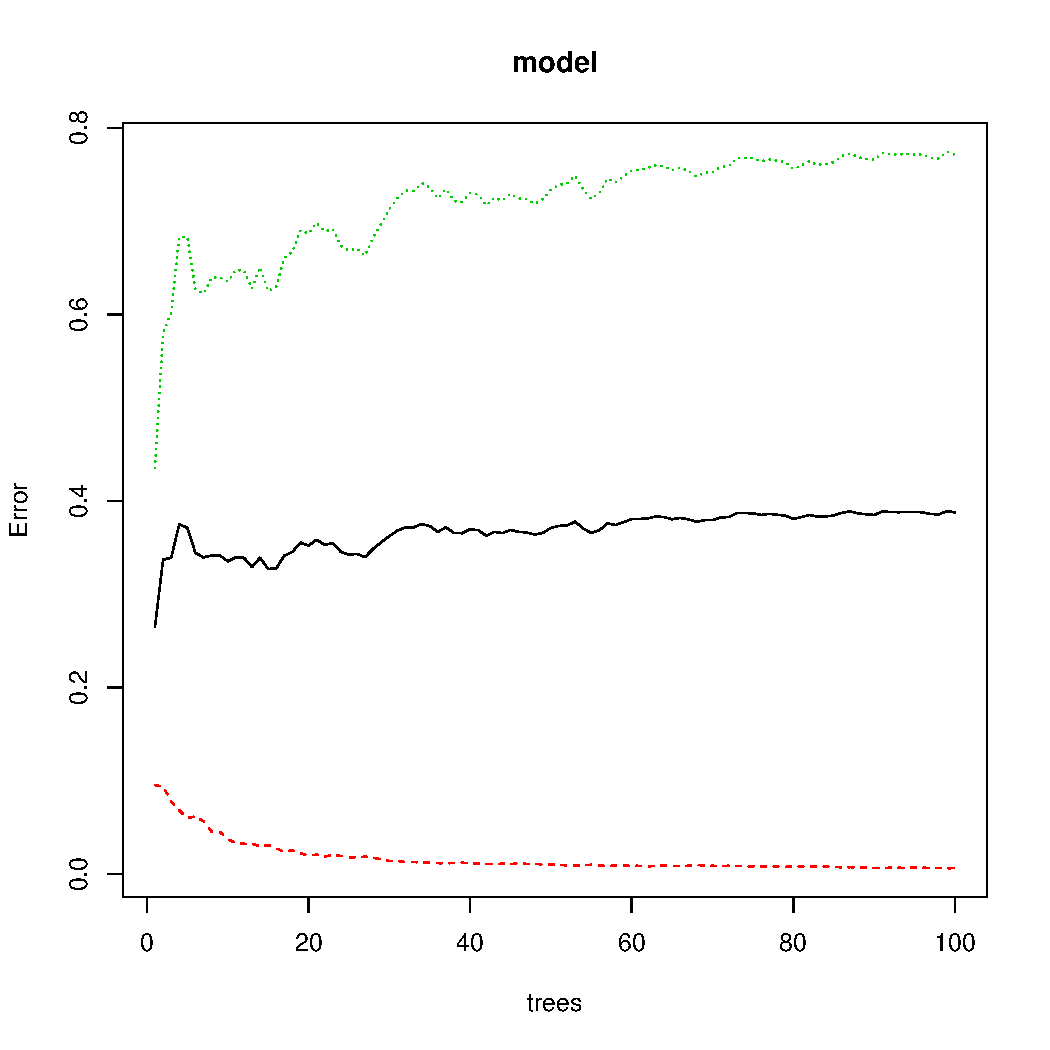
\includegraphics[width=\maxwidth]{figure/unnamed-chunk-28-1} 

\end{knitrout}
Now I will take a look at the error rates and accuracies of my model. During initial testing, accuracies where around 55-57 range. The train error rate tended to be lower than the test error rate but this was expected. The error rates for the CARAVAN=1 were extremely high, near 80 percent. Error rates for CARAVAN=0 Where extremely low less than 1 percent.This isn't great and could be improved. More data where CARAVAN=TRUE is really needed. Perhaps different resampling methods like bootstraping might generate better results. 

I will write a function to validate the model. I will use a 10 fold cross validation method.
\begin{knitrout}
\definecolor{shadecolor}{rgb}{0.969, 0.969, 0.969}\color{fgcolor}\begin{kframe}
\begin{alltt}
\hlcom{#Function to perform 10 fold cross validation}
\hlstd{validateModel} \hlkwb{<-} \hlkwa{function}\hlstd{(}\hlkwc{data}\hlstd{,}\hlkwc{ntrees}\hlstd{=}\hlnum{100}\hlstd{,}\hlkwc{nodeSize}\hlstd{=}\hlnum{1}\hlstd{)\{}
  \hlcom{#Frame to hold results}
  \hlstd{results}\hlkwb{<-}\hlkwd{data.frame}\hlstd{(}\hlkwc{OOB}\hlstd{=}\hlkwd{as.numeric}\hlstd{(),}
                      \hlkwc{trainFalseError}\hlstd{=}\hlkwd{as.numeric}\hlstd{(),}
                      \hlkwc{trainTrueError}\hlstd{=}\hlkwd{as.numeric}\hlstd{(),}
                      \hlkwc{testError}\hlstd{=}\hlkwd{as.numeric}\hlstd{(),}
                      \hlkwc{testFalseError}\hlstd{=}\hlkwd{as.numeric}\hlstd{(),}
                      \hlkwc{testTrueError}\hlstd{=}\hlkwd{as.numeric}\hlstd{(),}
                      \hlkwc{trainAccuracy}\hlstd{=}\hlkwd{as.numeric}\hlstd{(),}
                      \hlkwc{testAccuracy}\hlstd{=}\hlkwd{as.numeric}\hlstd{())}
  \hlcom{#Folds generated using Caret packages createFolds }
  \hlstd{folds}\hlkwb{<-}\hlkwd{createFolds}\hlstd{(data}\hlopt{$}\hlstd{CARAVAN,}\hlkwc{k}\hlstd{=}\hlnum{10}\hlstd{,}\hlkwc{list}\hlstd{=}\hlnum{TRUE}\hlstd{,}\hlkwc{returnTrain}\hlstd{=}\hlnum{FALSE}\hlstd{)}
  \hlkwa{for} \hlstd{(i} \hlkwa{in} \hlnum{1}\hlopt{:}\hlnum{10}\hlstd{)\{}
    \hlcom{#Keep one set for testing, rest training}
    \hlstd{trainData}\hlkwb{<-}\hlstd{data[}\hlopt{-}\hlkwd{c}\hlstd{(folds[[i]]),]}
    \hlstd{testData}\hlkwb{<-}\hlstd{data[}\hlkwd{c}\hlstd{(folds[[i]]),]}
    \hlstd{model}\hlkwb{<-}\hlkwd{randomForest}\hlstd{(trainData[,}\hlopt{-}\hlkwd{ncol}\hlstd{(trainData)],}
                        \hlstd{trainData[,}\hlkwd{ncol}\hlstd{(trainData)],}
                        \hlkwc{xtest}\hlstd{=testData[,}\hlopt{-}\hlkwd{ncol}\hlstd{(testData)],}
                        \hlkwc{ytest}\hlstd{=testData[,}\hlkwd{ncol}\hlstd{(testData)],}
                        \hlkwc{ntree}\hlstd{=ntrees,}
                        \hlkwc{nodesize}\hlstd{=nodeSize,}
                        \hlkwc{proximity}\hlstd{=}\hlnum{TRUE}\hlstd{)}
    \hlcom{#TRAIN}
    \hlstd{oob}\hlkwb{<-}\hlstd{model}\hlopt{$}\hlstd{err.rate[}\hlkwd{nrow}\hlstd{(model}\hlopt{$}\hlstd{test}\hlopt{$}\hlstd{err.rate),}\hlnum{1}\hlstd{,}\hlkwc{drop}\hlstd{=}\hlnum{FALSE}\hlstd{]}
    \hlstd{trainFalse}\hlkwb{<-}\hlstd{model}\hlopt{$}\hlstd{err.rate[}\hlkwd{nrow}\hlstd{(model}\hlopt{$}\hlstd{test}\hlopt{$}\hlstd{err.rate),}\hlnum{2}\hlstd{,}\hlkwc{drop}\hlstd{=}\hlnum{FALSE}\hlstd{]}
    \hlstd{trainTrue}\hlkwb{<-}\hlstd{model}\hlopt{$}\hlstd{err.rate[}\hlkwd{nrow}\hlstd{(model}\hlopt{$}\hlstd{test}\hlopt{$}\hlstd{err.rate),}\hlnum{3}\hlstd{,}\hlkwc{drop}\hlstd{=}\hlnum{FALSE}\hlstd{]}
    \hlstd{trainAccuracy}\hlkwb{<-}\hlkwd{sum}\hlstd{(}\hlkwd{diag}\hlstd{(model}\hlopt{$}\hlstd{confusion))}\hlopt{/}\hlkwd{nrow}\hlstd{(trainData)}
    \hlcom{#TEST}
    \hlstd{testError}\hlkwb{<-}\hlstd{model}\hlopt{$}\hlstd{test}\hlopt{$}\hlstd{err.rate[}\hlkwd{nrow}\hlstd{(model}\hlopt{$}\hlstd{test}\hlopt{$}\hlstd{err.rate),}\hlnum{1}\hlstd{,}\hlkwc{drop}\hlstd{=}\hlnum{FALSE}\hlstd{]}
    \hlstd{testFalse}\hlkwb{<-}\hlstd{model}\hlopt{$}\hlstd{test}\hlopt{$}\hlstd{err.rate[}\hlkwd{nrow}\hlstd{(model}\hlopt{$}\hlstd{test}\hlopt{$}\hlstd{err.rate),}\hlnum{2}\hlstd{,}\hlkwc{drop}\hlstd{=}\hlnum{FALSE}\hlstd{]}
    \hlstd{testTrue}\hlkwb{<-}\hlstd{model}\hlopt{$}\hlstd{test}\hlopt{$}\hlstd{err.rate[}\hlkwd{nrow}\hlstd{(model}\hlopt{$}\hlstd{test}\hlopt{$}\hlstd{err.rate),}\hlnum{3}\hlstd{,}\hlkwc{drop}\hlstd{=}\hlnum{FALSE}\hlstd{]}
    \hlstd{testAccuracy}\hlkwb{<-}\hlkwd{sum}\hlstd{(}\hlkwd{diag}\hlstd{(model}\hlopt{$}\hlstd{test}\hlopt{$}\hlstd{confusion))}\hlopt{/}\hlkwd{nrow}\hlstd{(testData)}
    \hlcom{#Create new Row in results with values}
    \hlstd{results[}\hlkwd{nrow}\hlstd{(results)}\hlopt{+}\hlnum{1}\hlstd{,]}\hlkwb{<-}\hlkwd{c}\hlstd{(oob,}
                                 \hlstd{trainFalse,}
                                 \hlstd{trainTrue,}
                                 \hlstd{testError,}
                                 \hlstd{testFalse,}
                                 \hlstd{testTrue,}
                                 \hlstd{trainAccuracy,}
                                 \hlstd{testAccuracy)}
  \hlstd{\}}
  \hlcom{#Return results}
  \hlkwd{return}\hlstd{(results)}
\hlstd{\}}
\end{alltt}
\end{kframe}
\end{knitrout}
I will also write a function to display the results. I will display the data frame as well as averages. 
\begin{knitrout}
\definecolor{shadecolor}{rgb}{0.969, 0.969, 0.969}\color{fgcolor}\begin{kframe}
\begin{alltt}
\hlcom{#Takes results and displays them as a whole and with averages }
\hlstd{displayResults}\hlkwb{<-}\hlkwa{function}\hlstd{(}\hlkwc{results}\hlstd{)\{}
  \hlstd{Position}\hlkwb{=}\hlkwd{c}\hlstd{(}\hlnum{1}\hlopt{:}\hlnum{10}\hlstd{)}
  \hlcom{#PLOT COLUMNS}
  \hlcom{#TRAIN}
  \hlcom{#OOB}
  \hlstd{plot}\hlkwb{<-}\hlkwd{ggplot}\hlstd{(results,}\hlkwd{aes}\hlstd{(}\hlkwc{x}\hlstd{=Position,}\hlkwc{y}\hlstd{=OOB))}
  \hlstd{plot}\hlkwb{<-}\hlstd{plot} \hlopt{+} \hlkwd{geom_point}\hlstd{()}
  \hlstd{plot}\hlkwb{<-}\hlstd{plot} \hlopt{+} \hlkwd{geom_smooth}\hlstd{()}
  \hlstd{plot}\hlkwb{<-}\hlstd{plot} \hlopt{+} \hlkwd{labs}\hlstd{(}\hlkwc{title}\hlstd{=}\hlstr{"OOB"}\hlstd{)}
  \hlkwd{print}\hlstd{(plot)}
  \hlcom{#Train Caravan=0 Error}
  \hlstd{plot}\hlkwb{<-}\hlkwd{ggplot}\hlstd{(results,}\hlkwd{aes}\hlstd{(}\hlkwc{x}\hlstd{=Position,}\hlkwc{y}\hlstd{=trainFalseError))}
  \hlstd{plot}\hlkwb{<-}\hlstd{plot} \hlopt{+} \hlkwd{geom_point}\hlstd{()}
  \hlstd{plot}\hlkwb{<-}\hlstd{plot} \hlopt{+} \hlkwd{geom_smooth}\hlstd{()}
  \hlstd{plot}\hlkwb{<-}\hlstd{plot} \hlopt{+} \hlkwd{labs}\hlstd{(}\hlkwc{title}\hlstd{=}\hlstr{"Train Caravan=0 Error"}\hlstd{)}
  \hlkwd{print}\hlstd{(plot)}
  \hlcom{#Train Caravan=1 Error}
  \hlstd{plot}\hlkwb{<-}\hlkwd{ggplot}\hlstd{(results,}\hlkwd{aes}\hlstd{(}\hlkwc{x}\hlstd{=Position,}\hlkwc{y}\hlstd{=trainTrueError))}
  \hlstd{plot}\hlkwb{<-}\hlstd{plot} \hlopt{+} \hlkwd{geom_point}\hlstd{()}
  \hlstd{plot}\hlkwb{<-}\hlstd{plot} \hlopt{+} \hlkwd{geom_smooth}\hlstd{()}
  \hlstd{plot}\hlkwb{<-}\hlstd{plot} \hlopt{+} \hlkwd{labs}\hlstd{(}\hlkwc{title}\hlstd{=}\hlstr{"Train Caravan=1 Error"}\hlstd{)}
  \hlkwd{print}\hlstd{(plot)}
  \hlcom{#Train Accuracy}
  \hlstd{plot}\hlkwb{<-}\hlkwd{ggplot}\hlstd{(results,}\hlkwd{aes}\hlstd{(}\hlkwc{x}\hlstd{=Position,}\hlkwc{y}\hlstd{=trainAccuracy))}
  \hlstd{plot}\hlkwb{<-}\hlstd{plot} \hlopt{+} \hlkwd{geom_point}\hlstd{()}
  \hlstd{plot}\hlkwb{<-}\hlstd{plot} \hlopt{+} \hlkwd{geom_smooth}\hlstd{()}
  \hlstd{plot}\hlkwb{<-}\hlstd{plot} \hlopt{+} \hlkwd{labs}\hlstd{(}\hlkwc{title}\hlstd{=}\hlstr{"Train Accuracy"}\hlstd{)}
  \hlkwd{print}\hlstd{(plot)}

  \hlcom{#TEST}
  \hlcom{#Test Error}
  \hlstd{plot}\hlkwb{<-}\hlkwd{ggplot}\hlstd{(results,}\hlkwd{aes}\hlstd{(}\hlkwc{x}\hlstd{=Position,}\hlkwc{y}\hlstd{=testError))}
  \hlstd{plot}\hlkwb{<-}\hlstd{plot} \hlopt{+} \hlkwd{geom_point}\hlstd{()}
  \hlstd{plot}\hlkwb{<-}\hlstd{plot} \hlopt{+} \hlkwd{geom_smooth}\hlstd{()}
  \hlstd{plot}\hlkwb{<-}\hlstd{plot} \hlopt{+} \hlkwd{labs}\hlstd{(}\hlkwc{title}\hlstd{=}\hlstr{"Test Error"}\hlstd{)}
  \hlkwd{print}\hlstd{(plot)}
  \hlcom{#Test Caravan=0 Error}
  \hlstd{plot}\hlkwb{<-}\hlkwd{ggplot}\hlstd{(results,}\hlkwd{aes}\hlstd{(}\hlkwc{x}\hlstd{=Position,}\hlkwc{y}\hlstd{=testFalseError))}
  \hlstd{plot}\hlkwb{<-}\hlstd{plot} \hlopt{+} \hlkwd{geom_point}\hlstd{()}
  \hlstd{plot}\hlkwb{<-}\hlstd{plot} \hlopt{+} \hlkwd{geom_smooth}\hlstd{()}
  \hlstd{plot}\hlkwb{<-}\hlstd{plot} \hlopt{+} \hlkwd{labs}\hlstd{(}\hlkwc{title}\hlstd{=}\hlstr{"Test Caravan=0 Error"}\hlstd{)}
  \hlkwd{print}\hlstd{(plot)}
  \hlcom{#Test Caravan=1 Error}
  \hlstd{plot}\hlkwb{<-}\hlkwd{ggplot}\hlstd{(results,}\hlkwd{aes}\hlstd{(}\hlkwc{x}\hlstd{=Position,}\hlkwc{y}\hlstd{=testTrueError))}
  \hlstd{plot}\hlkwb{<-}\hlstd{plot} \hlopt{+} \hlkwd{geom_point}\hlstd{()}
  \hlstd{plot}\hlkwb{<-}\hlstd{plot} \hlopt{+} \hlkwd{geom_smooth}\hlstd{()}
  \hlstd{plot}\hlkwb{<-}\hlstd{plot} \hlopt{+} \hlkwd{labs}\hlstd{(}\hlkwc{title}\hlstd{=}\hlstr{"Test Caravan=1 Error"}\hlstd{)}
  \hlkwd{print}\hlstd{(plot)}
  \hlcom{#Test Accuracy}
  \hlstd{plot}\hlkwb{<-}\hlkwd{ggplot}\hlstd{(results,}\hlkwd{aes}\hlstd{(}\hlkwc{x}\hlstd{=Position,}\hlkwc{y}\hlstd{=testAccuracy))}
  \hlstd{plot}\hlkwb{<-}\hlstd{plot} \hlopt{+} \hlkwd{geom_point}\hlstd{()}
  \hlstd{plot}\hlkwb{<-}\hlstd{plot} \hlopt{+} \hlkwd{geom_smooth}\hlstd{()}
  \hlstd{plot}\hlkwb{<-}\hlstd{plot} \hlopt{+} \hlkwd{labs}\hlstd{(}\hlkwc{title}\hlstd{=}\hlstr{"Test Accuracy"}\hlstd{)}
  \hlkwd{print}\hlstd{(plot)}

  \hlcom{#AVERAGES}
  \hlcom{#TRAIN}
  \hlcom{#OOB}
  \hlkwd{print}\hlstd{(}\hlkwd{paste}\hlstd{(}\hlstr{"Average OOB: "}\hlstd{,}
              \hlkwd{sum}\hlstd{(results}\hlopt{$}\hlstd{OOB)}\hlopt{/}\hlkwd{nrow}\hlstd{(results),}\hlkwc{sep}\hlstd{=}\hlstr{""}\hlstd{))}
  \hlcom{#Train CARAVAN=0 Error}
  \hlkwd{print}\hlstd{(}\hlkwd{paste}\hlstd{(}\hlstr{"Average CARAVAN=0 Error: "}\hlstd{,}
              \hlkwd{sum}\hlstd{(results}\hlopt{$}\hlstd{trainFalseError)}\hlopt{/}\hlkwd{nrow}\hlstd{(results),}\hlkwc{sep}\hlstd{=}\hlstr{""}\hlstd{))}
  \hlcom{#Train Caravan=1 Error}
  \hlkwd{print}\hlstd{(}\hlkwd{paste}\hlstd{(}\hlstr{"Average CARAVAN=1 Error: "}\hlstd{,}
              \hlkwd{sum}\hlstd{(results}\hlopt{$}\hlstd{trainTrueError)}\hlopt{/}\hlkwd{nrow}\hlstd{(results),}\hlkwc{sep}\hlstd{=}\hlstr{""}\hlstd{))}
  \hlcom{#Train Accuracy}
  \hlkwd{print}\hlstd{(}\hlkwd{paste}\hlstd{(}\hlstr{"Average Train Accuracy: "}\hlstd{,}
              \hlkwd{sum}\hlstd{(results}\hlopt{$}\hlstd{trainAccuracy)}\hlopt{/}\hlkwd{nrow}\hlstd{(results),}\hlkwc{sep}\hlstd{=}\hlstr{""}\hlstd{))}

  \hlcom{#Print blank line between train and test results}
  \hlkwd{print}\hlstd{(}\hlstr{" "}\hlstd{)}

  \hlcom{#Test Error}
  \hlkwd{print}\hlstd{(}\hlkwd{paste}\hlstd{(}\hlstr{"Average Test Error: "}\hlstd{,}
              \hlkwd{sum}\hlstd{(results}\hlopt{$}\hlstd{testError)}\hlopt{/}\hlkwd{nrow}\hlstd{(results),}\hlkwc{sep}\hlstd{=}\hlstr{""}\hlstd{))}
  \hlcom{#Test CARAVAN=0 Error}
  \hlkwd{print}\hlstd{(}\hlkwd{paste}\hlstd{(}\hlstr{"Average CARAVAN=0 Error: "}\hlstd{,}
              \hlkwd{sum}\hlstd{(results}\hlopt{$}\hlstd{testFalseError)}\hlopt{/}\hlkwd{nrow}\hlstd{(results),}\hlkwc{sep}\hlstd{=}\hlstr{""}\hlstd{))}
  \hlcom{#Test CARAVAN=1 Error}
  \hlkwd{print}\hlstd{(}\hlkwd{paste}\hlstd{(}\hlstr{"Average CARAVAN=1 Error: "}\hlstd{,}
              \hlkwd{sum}\hlstd{(results}\hlopt{$}\hlstd{testTrueError)}\hlopt{/}\hlkwd{nrow}\hlstd{(results),}\hlkwc{sep}\hlstd{=}\hlstr{""}\hlstd{))}
  \hlcom{#Test Accuracy}
  \hlkwd{print}\hlstd{(}\hlkwd{paste}\hlstd{(}\hlstr{"Average Test Accuracy: "}\hlstd{,}
              \hlkwd{sum}\hlstd{(results}\hlopt{$}\hlstd{testAccuracy)}\hlopt{/}\hlkwd{nrow}\hlstd{(results),}\hlkwc{sep}\hlstd{=}\hlstr{""}\hlstd{))}
\hlstd{\}}
\end{alltt}
\end{kframe}
\end{knitrout}
I will now use these functions to validate my model
\begin{knitrout}
\definecolor{shadecolor}{rgb}{0.969, 0.969, 0.969}\color{fgcolor}\begin{kframe}
\begin{alltt}
\hlcom{#Validate Model}
\hlstd{validateResult} \hlkwb{<-} \hlkwd{validateModel}\hlstd{(df)}
\hlkwd{displayResults}\hlstd{(validateResult)}
\end{alltt}


{\ttfamily\noindent\itshape\color{messagecolor}{\#\# `geom\_smooth()` using method = 'loess'}}\end{kframe}
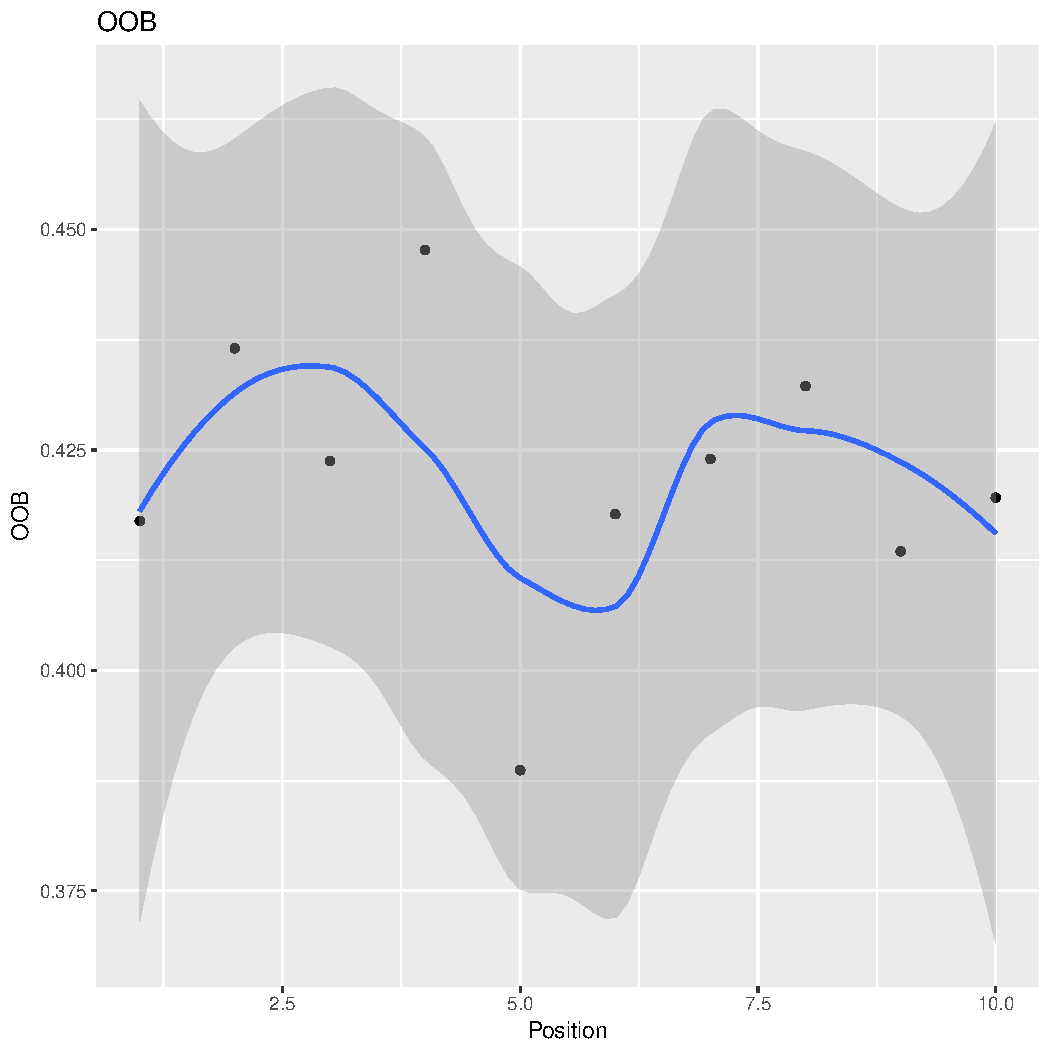
\includegraphics[width=\maxwidth]{figure/unnamed-chunk-31-1} 
\begin{kframe}

{\ttfamily\noindent\itshape\color{messagecolor}{\#\# `geom\_smooth()` using method = 'loess'}}\end{kframe}
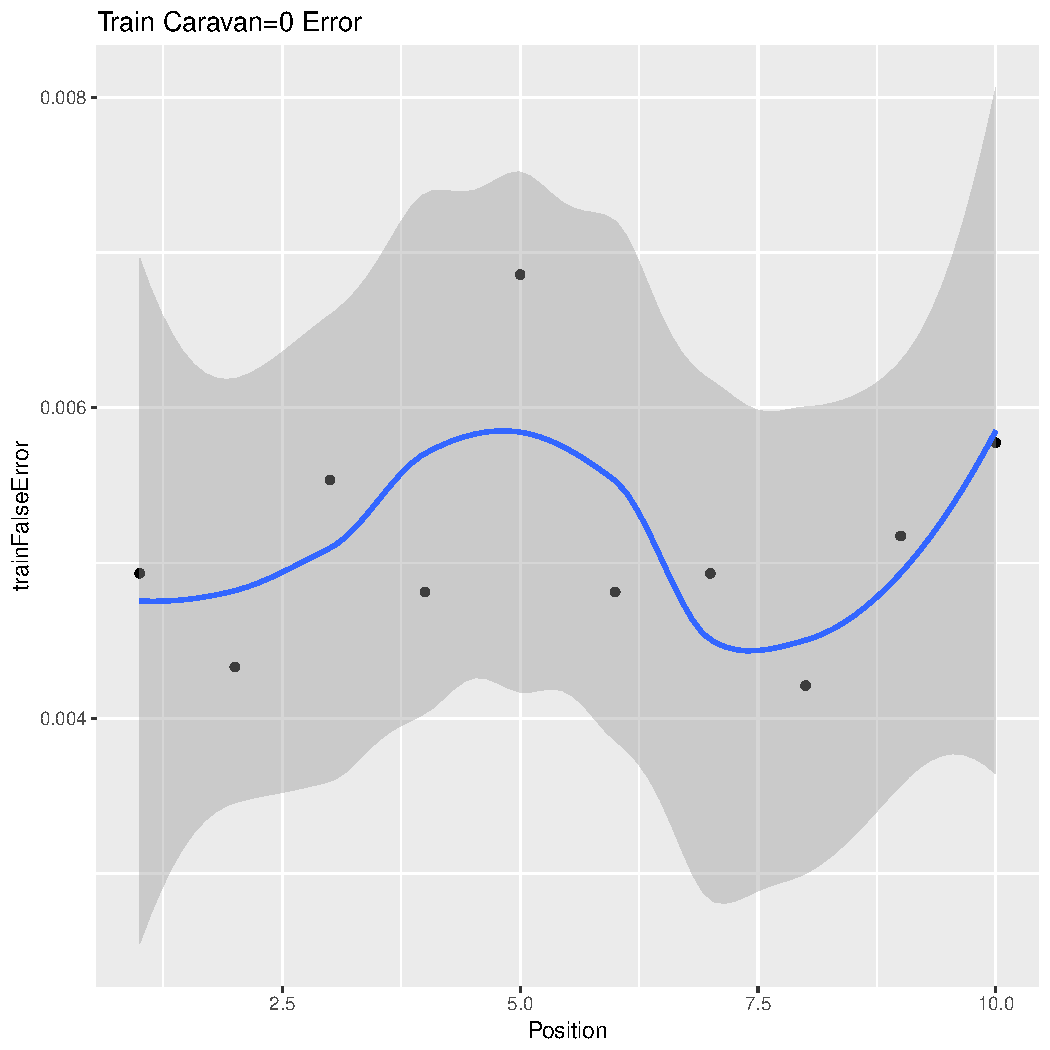
\includegraphics[width=\maxwidth]{figure/unnamed-chunk-31-2} 
\begin{kframe}

{\ttfamily\noindent\itshape\color{messagecolor}{\#\# `geom\_smooth()` using method = 'loess'}}\end{kframe}
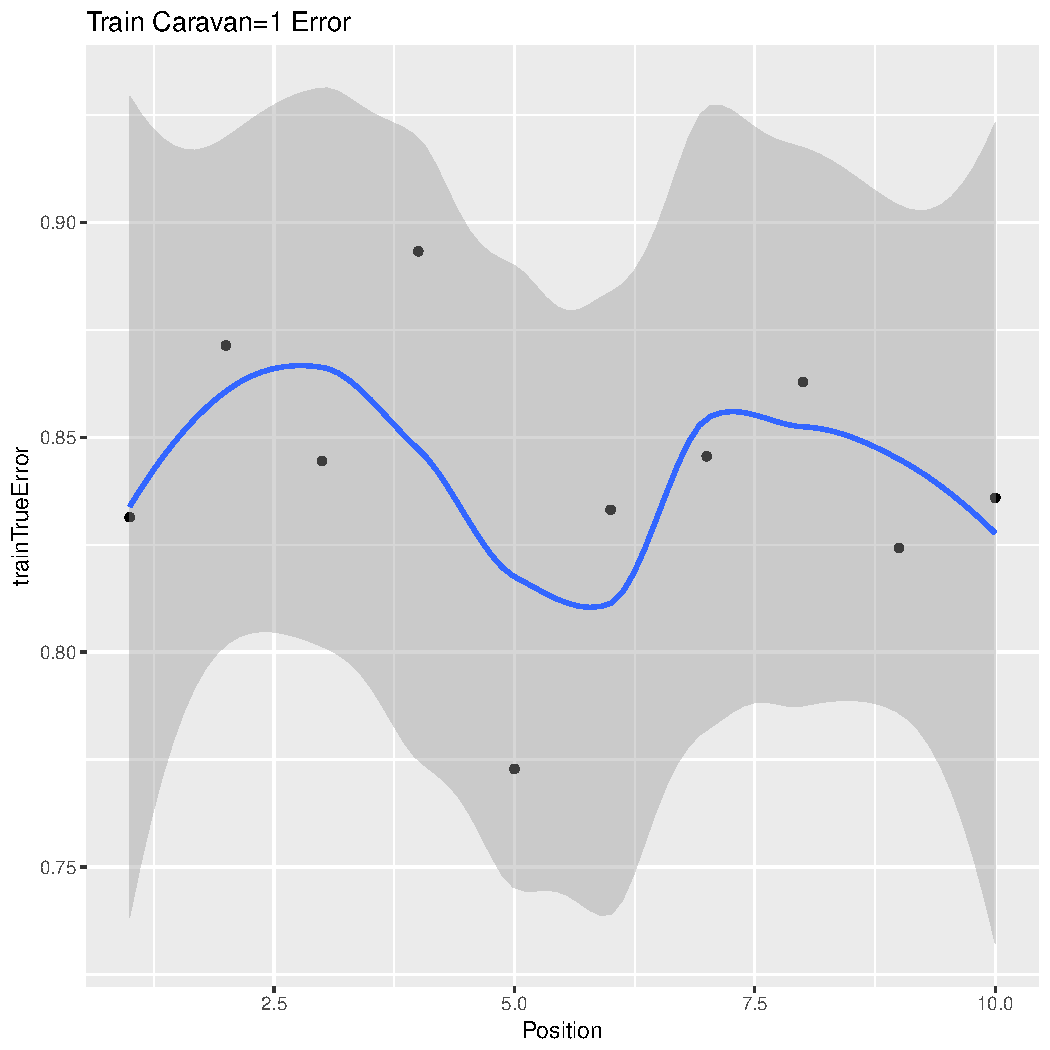
\includegraphics[width=\maxwidth]{figure/unnamed-chunk-31-3} 
\begin{kframe}

{\ttfamily\noindent\itshape\color{messagecolor}{\#\# `geom\_smooth()` using method = 'loess'}}\end{kframe}
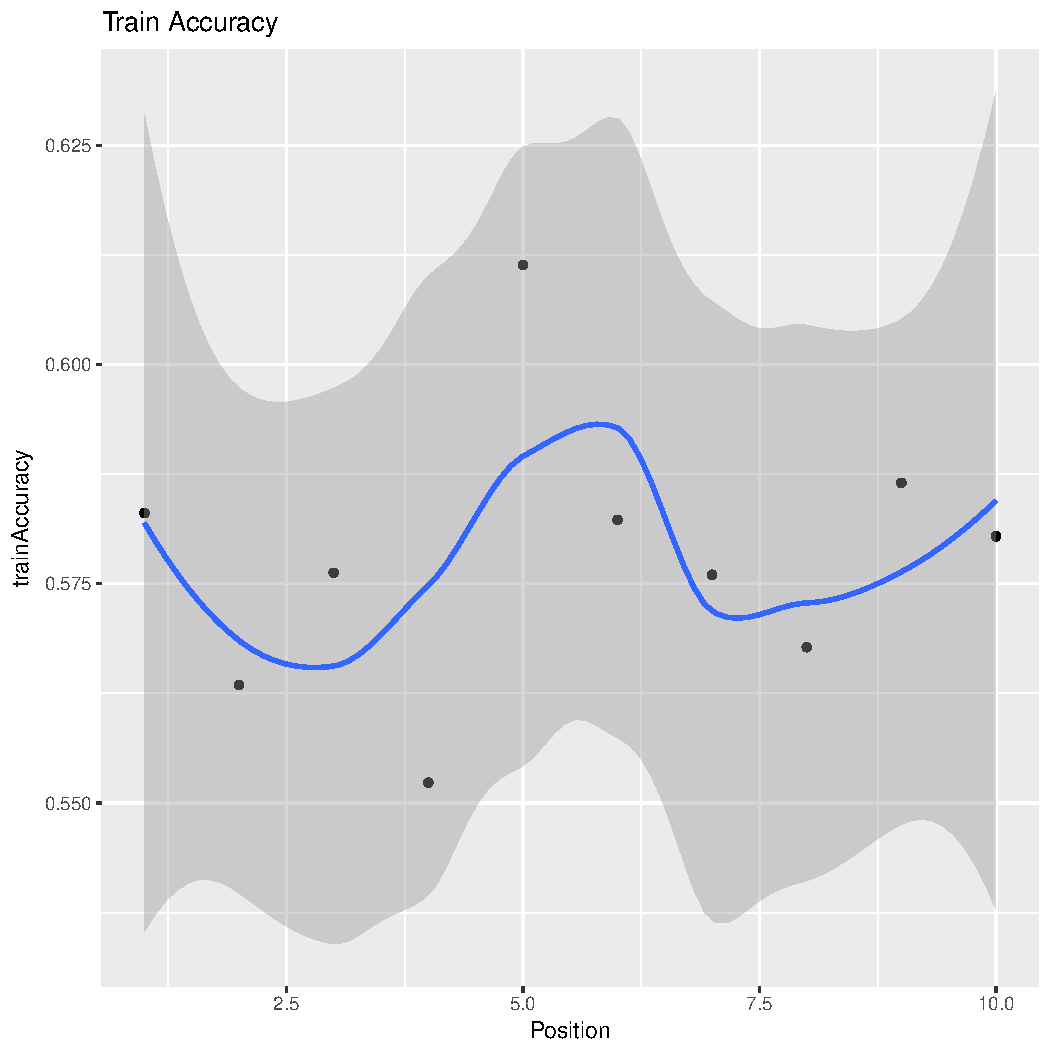
\includegraphics[width=\maxwidth]{figure/unnamed-chunk-31-4} 
\begin{kframe}

{\ttfamily\noindent\itshape\color{messagecolor}{\#\# `geom\_smooth()` using method = 'loess'}}\end{kframe}
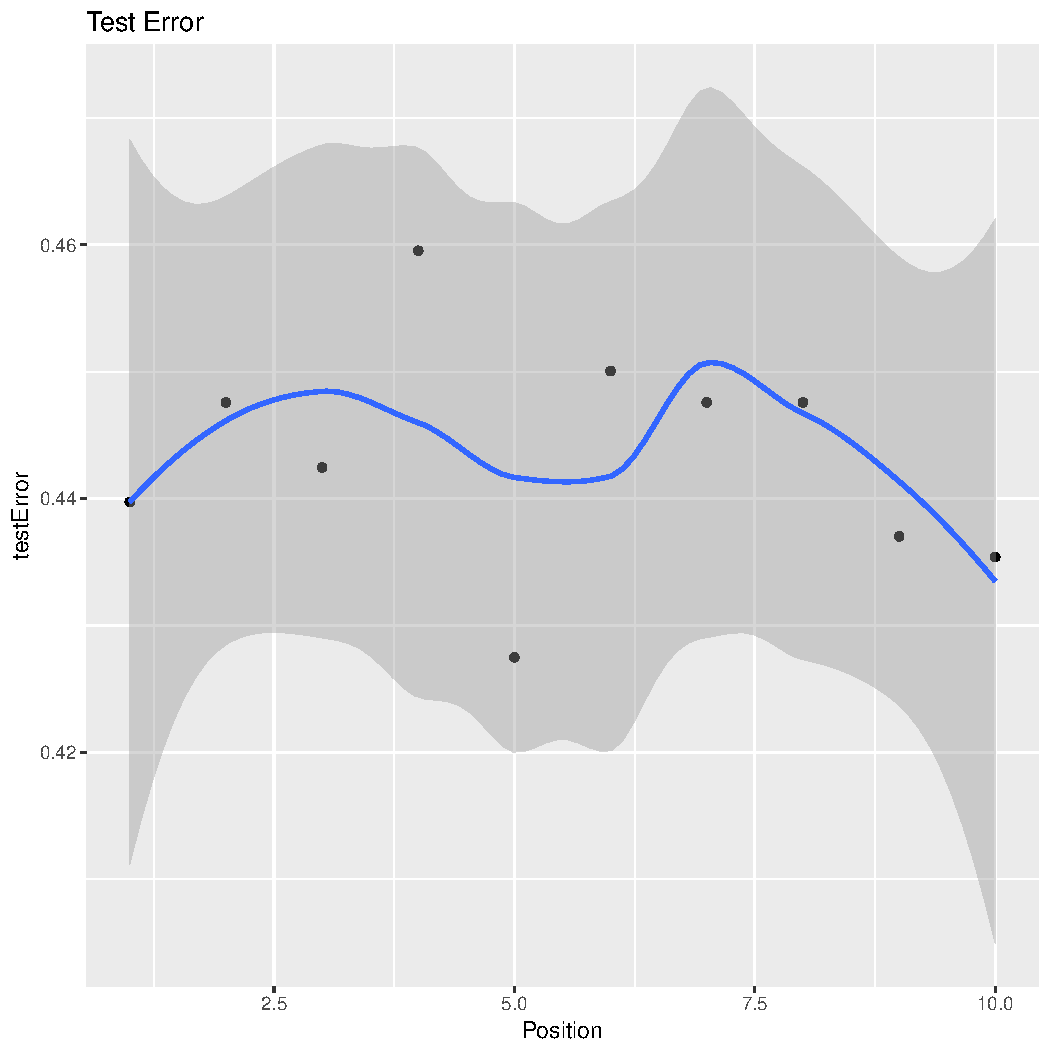
\includegraphics[width=\maxwidth]{figure/unnamed-chunk-31-5} 
\begin{kframe}

{\ttfamily\noindent\itshape\color{messagecolor}{\#\# `geom\_smooth()` using method = 'loess'}}\end{kframe}
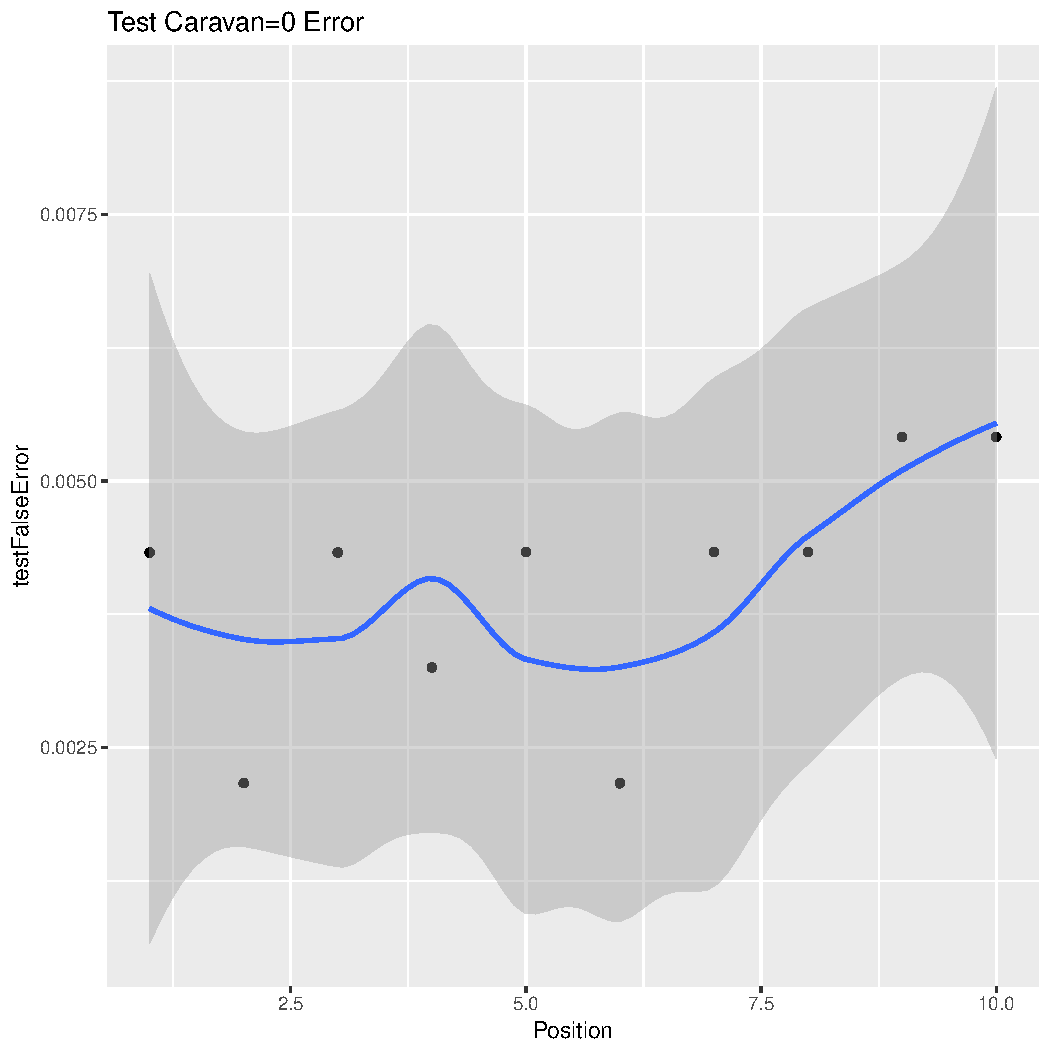
\includegraphics[width=\maxwidth]{figure/unnamed-chunk-31-6} 
\begin{kframe}

{\ttfamily\noindent\itshape\color{messagecolor}{\#\# `geom\_smooth()` using method = 'loess'}}\end{kframe}
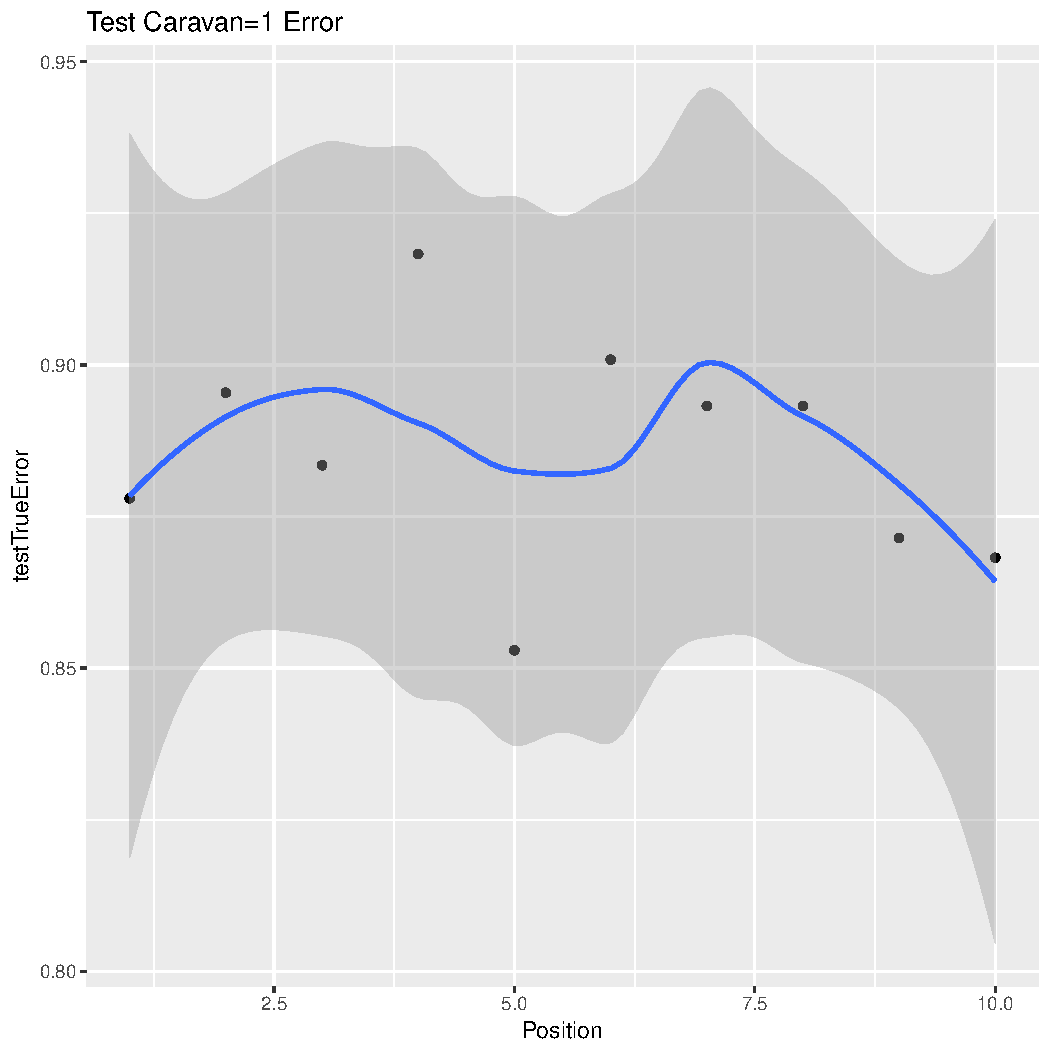
\includegraphics[width=\maxwidth]{figure/unnamed-chunk-31-7} 
\begin{kframe}

{\ttfamily\noindent\itshape\color{messagecolor}{\#\# `geom\_smooth()` using method = 'loess'}}\end{kframe}
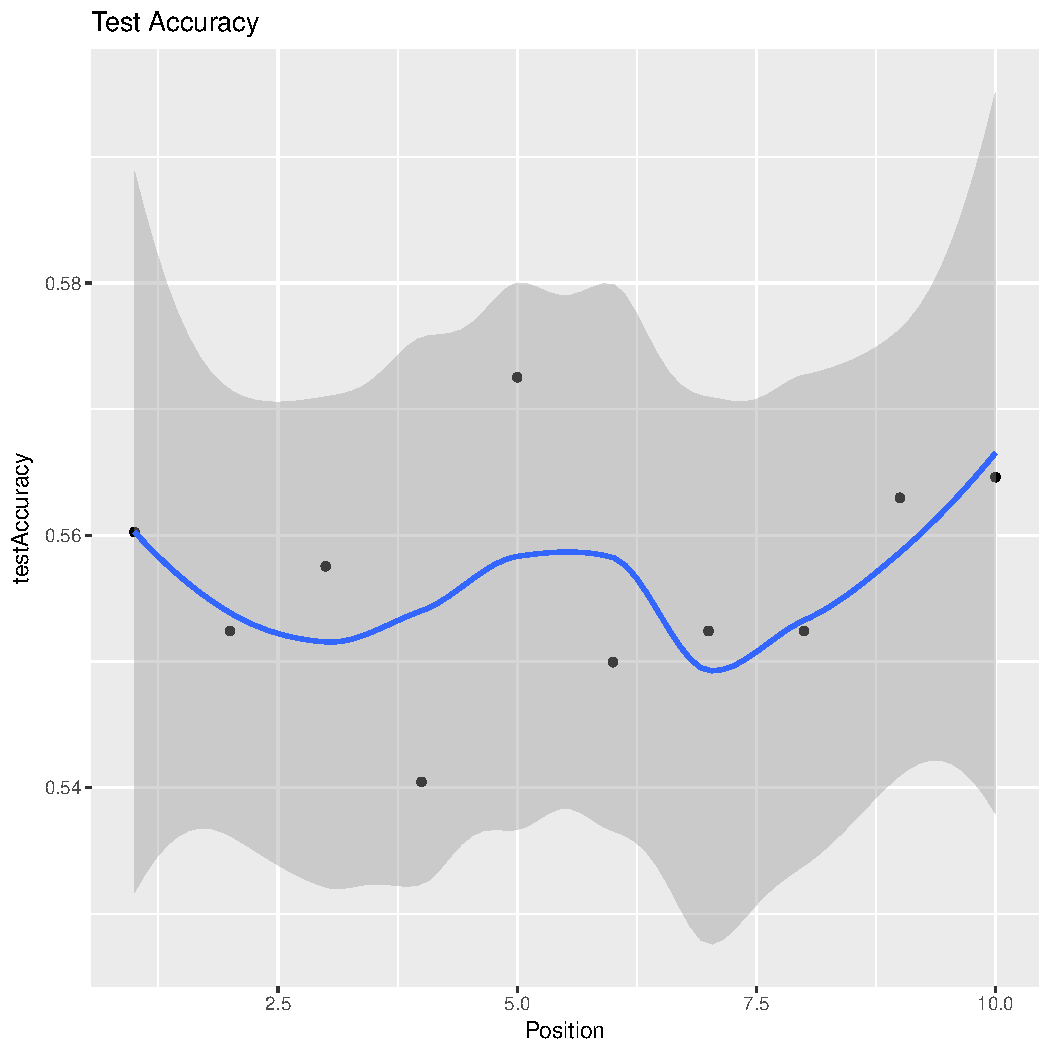
\includegraphics[width=\maxwidth]{figure/unnamed-chunk-31-8} 
\begin{kframe}\begin{verbatim}
## [1] "Average OOB: 0.422065231895882"
## [1] "Average CARAVAN=0 Error: 0.00513746667826271"
## [1] "Average CARAVAN=1 Error: 0.841491164366981"
## [1] "Average Train Accuracy: 0.577934768104118"
## [1] " "
## [1] "Average Test Error: 0.443443526950667"
## [1] "Average CARAVAN=0 Error: 0.00400632231618147"
## [1] "Average CARAVAN=1 Error: 0.885511982570806"
## [1] "Average Test Accuracy: 0.556556473049333"
\end{verbatim}
\end{kframe}
\end{knitrout}
Similar results to training the initial model, accuracies in the 55-57 range roughly. Although there isn't much variance in any of the values. Right now the model is almost just saying that all the rows are FALSE.Train accuracy was higher than test accuracy again. Train error rate for when CARAVAN=1 was extremely high, near 90 percent. Compared to when CARAVAN=0 which was < 1 percent. 
\section{Imporving Performance}
I will now try to improve the performance of my model 

I will start by tring to fine tune the ntrees attribute of my model by testing my model with values between 1 and 100 for ntree. I was originally going to use the range 100 to 1000 and increment by 100 trees, but during testing I found that the lowest accuracies where within the 1 too 100 range and that after 100 they only increased. I have set the increment to 10 as I don't want to overfit the model. 

I have chosen to try and fine tune this attribute as I know it has an effect on accuracy. Although I may accidently overfit the model by setting the value of ntree too low. I have found during testing that the higher the number of ntrees the greater the error rate. This is mostly due to the error rate when CARAVAN=1 increasing with the number of trees. The error rate for CARAVAN=0 tends to level out and become near linear. 

I will write a function to do this, that will return the optimal number of trees based on test accuracy.
\begin{knitrout}
\definecolor{shadecolor}{rgb}{0.969, 0.969, 0.969}\color{fgcolor}\begin{kframe}
\begin{alltt}
\hlcom{#Using same train and test set as before }
\hlcom{#Tweak number of trees }
\hlstd{testNTrees} \hlkwb{<-} \hlkwa{function}\hlstd{(}\hlkwc{trainData}\hlstd{,}\hlkwc{testData}\hlstd{)\{}
  \hlstd{ntrees}\hlkwb{<-}\hlnum{20}
  \hlstd{results}\hlkwb{<-}\hlkwa{NULL}
  \hlstd{results}\hlkwb{<-}\hlkwd{data.frame}\hlstd{(}\hlkwc{NTrees}\hlstd{=}\hlkwd{as.numeric}\hlstd{(),}
                      \hlkwc{OOB}\hlstd{=}\hlkwd{as.numeric}\hlstd{(),}
                      \hlkwc{trainFalseError}\hlstd{=}\hlkwd{as.numeric}\hlstd{(),}
                      \hlkwc{trainTrueError}\hlstd{=}\hlkwd{as.numeric}\hlstd{(),}
                      \hlkwc{testError}\hlstd{=}\hlkwd{as.numeric}\hlstd{(),}
                      \hlkwc{testFalseError}\hlstd{=}\hlkwd{as.numeric}\hlstd{(),}
                      \hlkwc{testTrueError}\hlstd{=}\hlkwd{as.numeric}\hlstd{(),}
                      \hlkwc{trainAccuracy}\hlstd{=}\hlkwd{as.numeric}\hlstd{(),}
                      \hlkwc{testAccuracy}\hlstd{=}\hlkwd{as.numeric}\hlstd{())}
  \hlkwa{for} \hlstd{(i} \hlkwa{in} \hlnum{1}\hlopt{:}\hlnum{9}\hlstd{)\{}
    \hlstd{trainData}\hlkwb{=}\hlstd{train}
    \hlstd{testData}\hlkwb{=}\hlstd{test}
    \hlstd{model}\hlkwb{<-}\hlkwd{randomForest}\hlstd{(trainData[,}\hlopt{-}\hlkwd{ncol}\hlstd{(trainData)],}
                        \hlstd{trainData[,}\hlkwd{ncol}\hlstd{(trainData)],}
                        \hlkwc{xtest}\hlstd{=testData[,}\hlopt{-}\hlkwd{ncol}\hlstd{(testData)],}
                        \hlkwc{ytest}\hlstd{=testData[,}\hlkwd{ncol}\hlstd{(testData)],}
                        \hlkwc{ntree}\hlstd{=ntrees,}
                        \hlkwc{proximity}\hlstd{=}\hlnum{TRUE}\hlstd{)}
    \hlcom{#TRAIN}
    \hlstd{oob}\hlkwb{<-}\hlstd{model}\hlopt{$}\hlstd{err.rate[}\hlkwd{nrow}\hlstd{(model}\hlopt{$}\hlstd{test}\hlopt{$}\hlstd{err.rate),}\hlnum{1}\hlstd{,}\hlkwc{drop}\hlstd{=}\hlnum{FALSE}\hlstd{]}
    \hlstd{trainFalse}\hlkwb{<-}\hlstd{model}\hlopt{$}\hlstd{err.rate[}\hlkwd{nrow}\hlstd{(model}\hlopt{$}\hlstd{test}\hlopt{$}\hlstd{err.rate),}\hlnum{2}\hlstd{,}\hlkwc{drop}\hlstd{=}\hlnum{FALSE}\hlstd{]}
    \hlstd{trainTrue}\hlkwb{<-}\hlstd{model}\hlopt{$}\hlstd{err.rate[}\hlkwd{nrow}\hlstd{(model}\hlopt{$}\hlstd{test}\hlopt{$}\hlstd{err.rate),}\hlnum{3}\hlstd{,}\hlkwc{drop}\hlstd{=}\hlnum{FALSE}\hlstd{]}
    \hlstd{trainAccuracy}\hlkwb{<-}\hlkwd{sum}\hlstd{(}\hlkwd{diag}\hlstd{(model}\hlopt{$}\hlstd{confusion))}\hlopt{/}\hlkwd{nrow}\hlstd{(trainData)}
    \hlcom{#TEST}
    \hlstd{testError}\hlkwb{<-}\hlstd{model}\hlopt{$}\hlstd{test}\hlopt{$}\hlstd{err.rate[}\hlkwd{nrow}\hlstd{(model}\hlopt{$}\hlstd{test}\hlopt{$}\hlstd{err.rate),}\hlnum{1}\hlstd{,}\hlkwc{drop}\hlstd{=}\hlnum{FALSE}\hlstd{]}
    \hlstd{testFalse}\hlkwb{<-}\hlstd{model}\hlopt{$}\hlstd{test}\hlopt{$}\hlstd{err.rate[}\hlkwd{nrow}\hlstd{(model}\hlopt{$}\hlstd{test}\hlopt{$}\hlstd{err.rate),}\hlnum{2}\hlstd{,}\hlkwc{drop}\hlstd{=}\hlnum{FALSE}\hlstd{]}
    \hlstd{testTrue}\hlkwb{<-}\hlstd{model}\hlopt{$}\hlstd{test}\hlopt{$}\hlstd{err.rate[}\hlkwd{nrow}\hlstd{(model}\hlopt{$}\hlstd{test}\hlopt{$}\hlstd{err.rate),}\hlnum{3}\hlstd{,}\hlkwc{drop}\hlstd{=}\hlnum{FALSE}\hlstd{]}
    \hlstd{testAccuracy}\hlkwb{<-}\hlkwd{sum}\hlstd{(}\hlkwd{diag}\hlstd{(model}\hlopt{$}\hlstd{test}\hlopt{$}\hlstd{confusion))}\hlopt{/}\hlkwd{nrow}\hlstd{(testData)}
    \hlcom{#Create new row in results with new data}
    \hlstd{results[}\hlkwd{nrow}\hlstd{(results)}\hlopt{+}\hlnum{1}\hlstd{,]}\hlkwb{<-}\hlkwd{c}\hlstd{(ntrees,}
                                 \hlstd{oob,}
                                 \hlstd{trainFalse,}
                                 \hlstd{trainTrue,}
                                 \hlstd{testError,}
                                 \hlstd{testFalse,}
                                 \hlstd{testTrue,}
                                 \hlstd{trainAccuracy,}
                                 \hlstd{testAccuracy)}
    \hlstd{results}
    \hlstd{ntrees} \hlkwb{<-}\hlstd{ntrees} \hlopt{+} \hlnum{10}
  \hlstd{\}}
  \hlcom{#return max row}
  \hlstd{ntrees}\hlkwb{<-}\hlstd{results}\hlopt{$}\hlstd{NTrees[}\hlkwd{which.max}\hlstd{(results}\hlopt{$}\hlstd{testAccuracy)]}
  \hlkwd{return}\hlstd{(ntrees)}
\hlstd{\}}
\end{alltt}
\end{kframe}
\end{knitrout}

I will now use this function to find ntrees. 
\begin{knitrout}
\definecolor{shadecolor}{rgb}{0.969, 0.969, 0.969}\color{fgcolor}\begin{kframe}
\begin{alltt}
\hlcom{#Get ntrees}
\hlstd{ntrees}\hlkwb{<-}\hlkwd{testNTrees}\hlstd{(train,test)}
\hlstd{ntrees}
\end{alltt}
\begin{verbatim}
## [1] 20
\end{verbatim}
\end{kframe}
\end{knitrout}
During testing, ntree values were not high. Usually 100 or 200 was returned 

I will not build a second model with the new values of ntrees to compare it to the original model
\begin{knitrout}
\definecolor{shadecolor}{rgb}{0.969, 0.969, 0.969}\color{fgcolor}\begin{kframe}
\begin{alltt}
\hlcom{#Build second model with new ntree and nodesize}
\hlstd{model2}\hlkwb{<-}\hlkwd{buildModel}\hlstd{(train,test,}\hlkwc{ntrees}\hlstd{=ntrees)}
\hlcom{#Display Values}
\hlkwd{displayResultsFromModel}\hlstd{(model2,}\hlkwd{nrow}\hlstd{(train),}\hlkwd{nrow}\hlstd{(test))}
\end{alltt}
\begin{verbatim}
## [1] "TRAIN"
## [1] "Train OOB Error: 0.352986811481769"
## [1] "Train CARAVAN=0 Error: 0.0165506573859242"
## [1] "Train CARAVAN=1 Error: 0.691517509727626"
## [1] "Train Accuracy: 0.646962997440074"
## [1] " "
## [1] "TEST"
## [1] "Test Error: 0.391564083997104"
## [1] "Test CARAVAN=0 Error: 0.0101083032490975"
## [1] "Test CARAVAN=1 Error: 0.77523602033406"
## [1] "Test Accuracy: 0.608435916002896"
\end{verbatim}
\begin{alltt}
\hlcom{#Plot Errors}
\hlkwd{plot}\hlstd{(model2)}
\end{alltt}
\end{kframe}
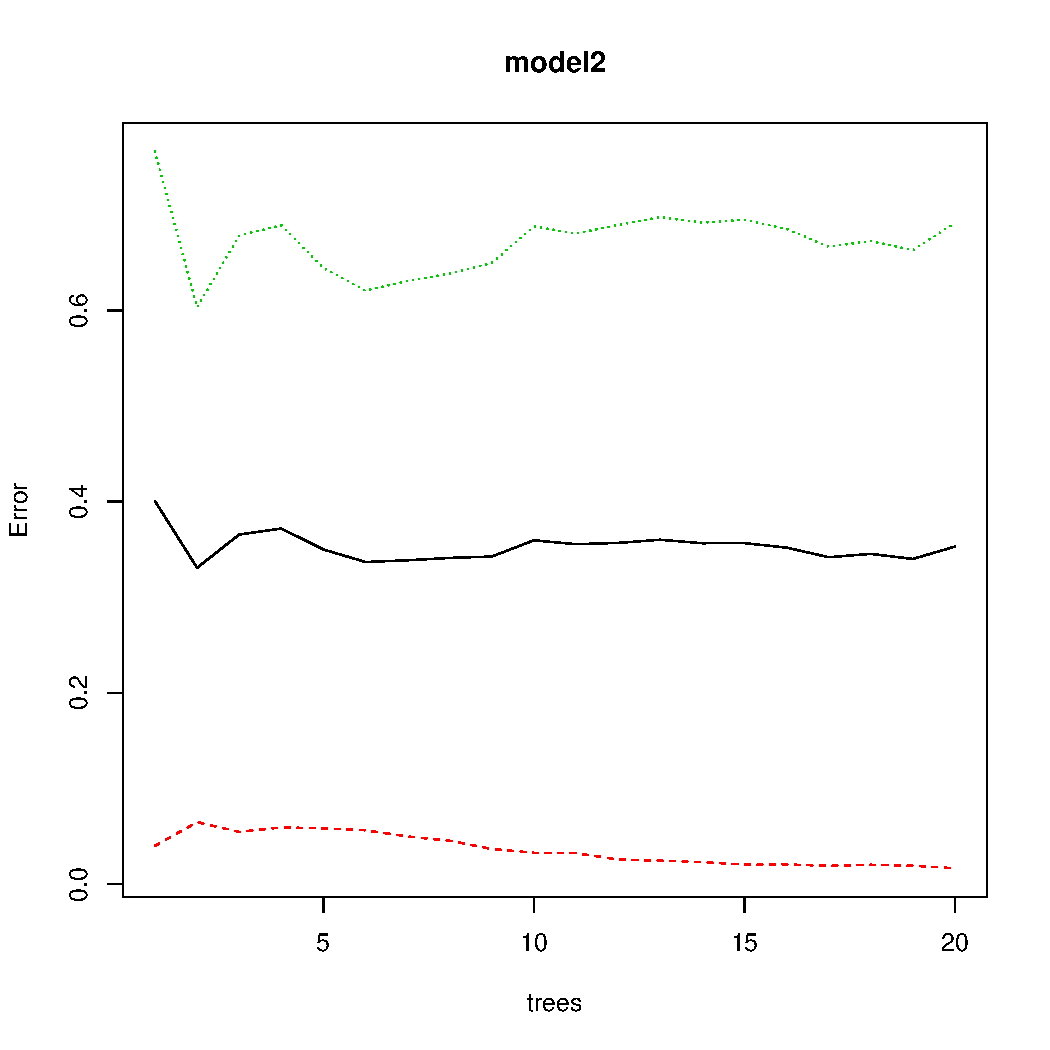
\includegraphics[width=\maxwidth]{figure/unnamed-chunk-34-1} 

\end{knitrout}

I will now validate the new model
\begin{knitrout}
\definecolor{shadecolor}{rgb}{0.969, 0.969, 0.969}\color{fgcolor}\begin{kframe}
\begin{alltt}
\hlcom{#Validate second model, 10 fold cross validation }
\hlstd{validateResults2}\hlkwb{<-}\hlkwd{validateModel}\hlstd{(df,ntrees)}
\hlkwd{displayResults}\hlstd{(validateResults2)}
\end{alltt}


{\ttfamily\noindent\itshape\color{messagecolor}{\#\# `geom\_smooth()` using method = 'loess'}}\end{kframe}
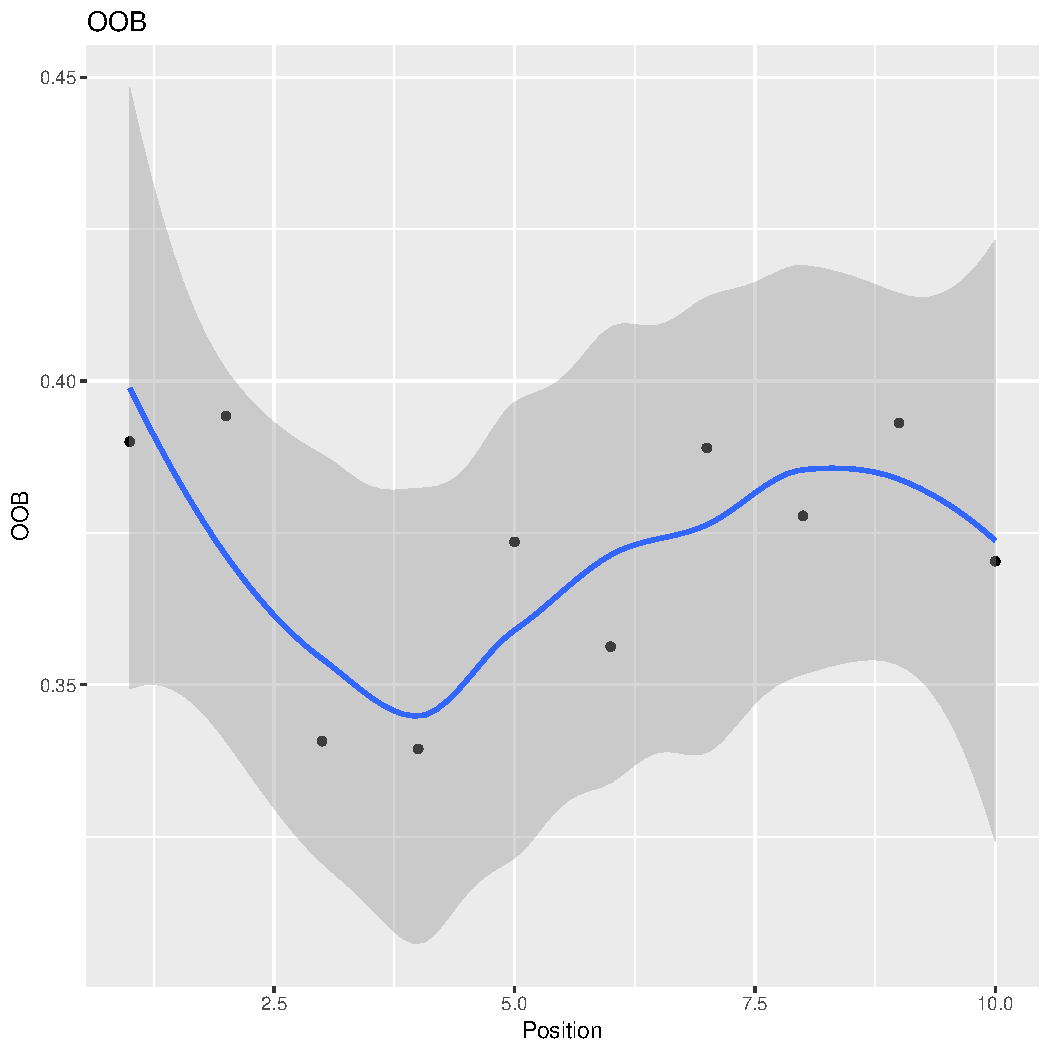
\includegraphics[width=\maxwidth]{figure/unnamed-chunk-35-1} 
\begin{kframe}

{\ttfamily\noindent\itshape\color{messagecolor}{\#\# `geom\_smooth()` using method = 'loess'}}\end{kframe}
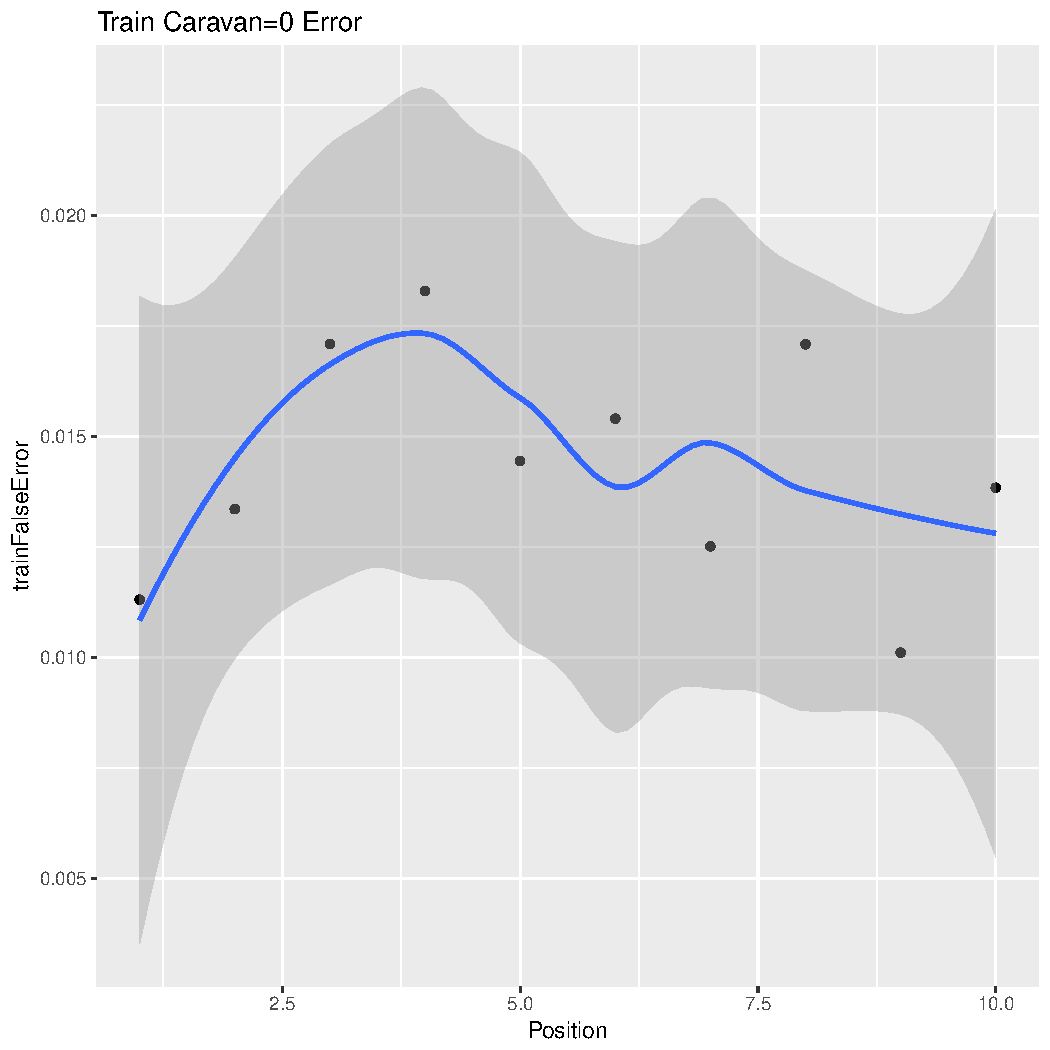
\includegraphics[width=\maxwidth]{figure/unnamed-chunk-35-2} 
\begin{kframe}

{\ttfamily\noindent\itshape\color{messagecolor}{\#\# `geom\_smooth()` using method = 'loess'}}\end{kframe}
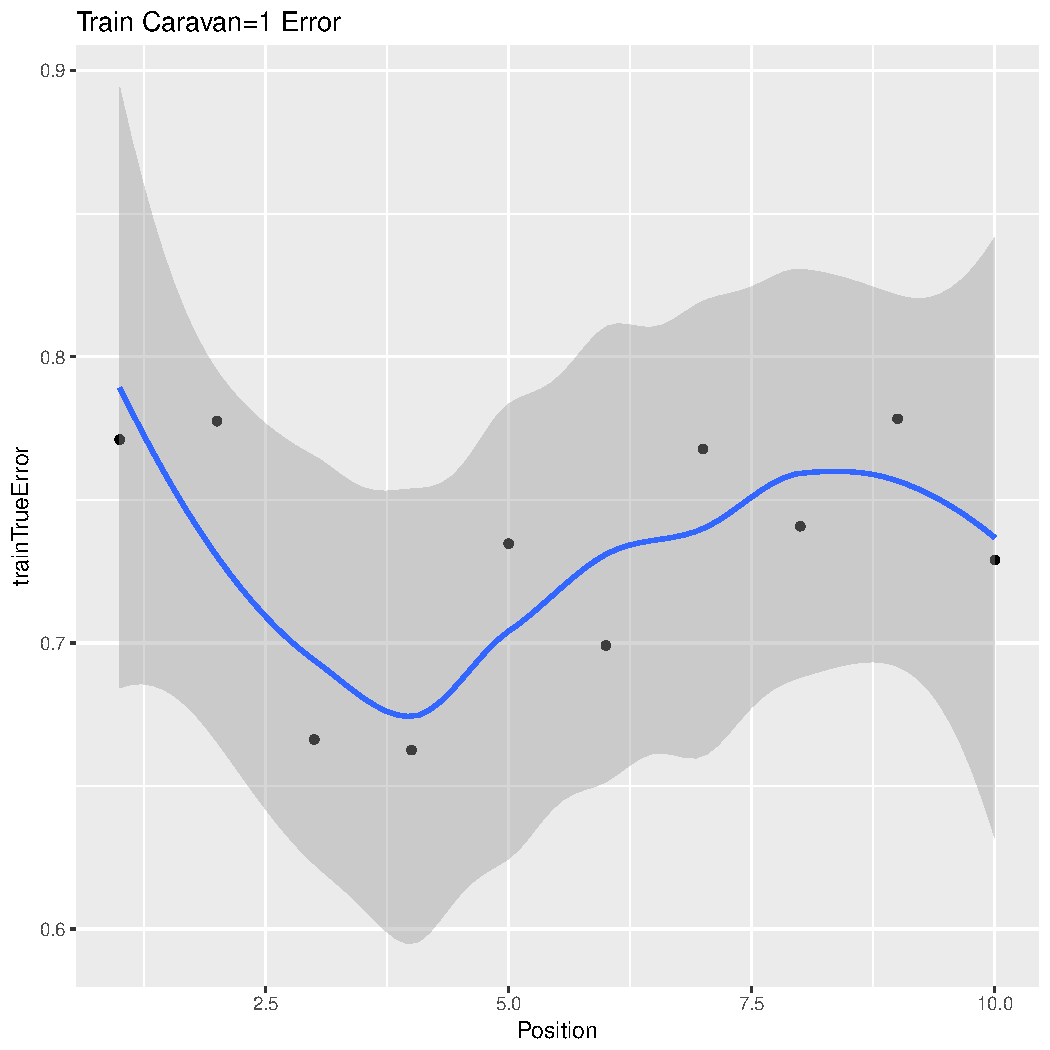
\includegraphics[width=\maxwidth]{figure/unnamed-chunk-35-3} 
\begin{kframe}

{\ttfamily\noindent\itshape\color{messagecolor}{\#\# `geom\_smooth()` using method = 'loess'}}\end{kframe}
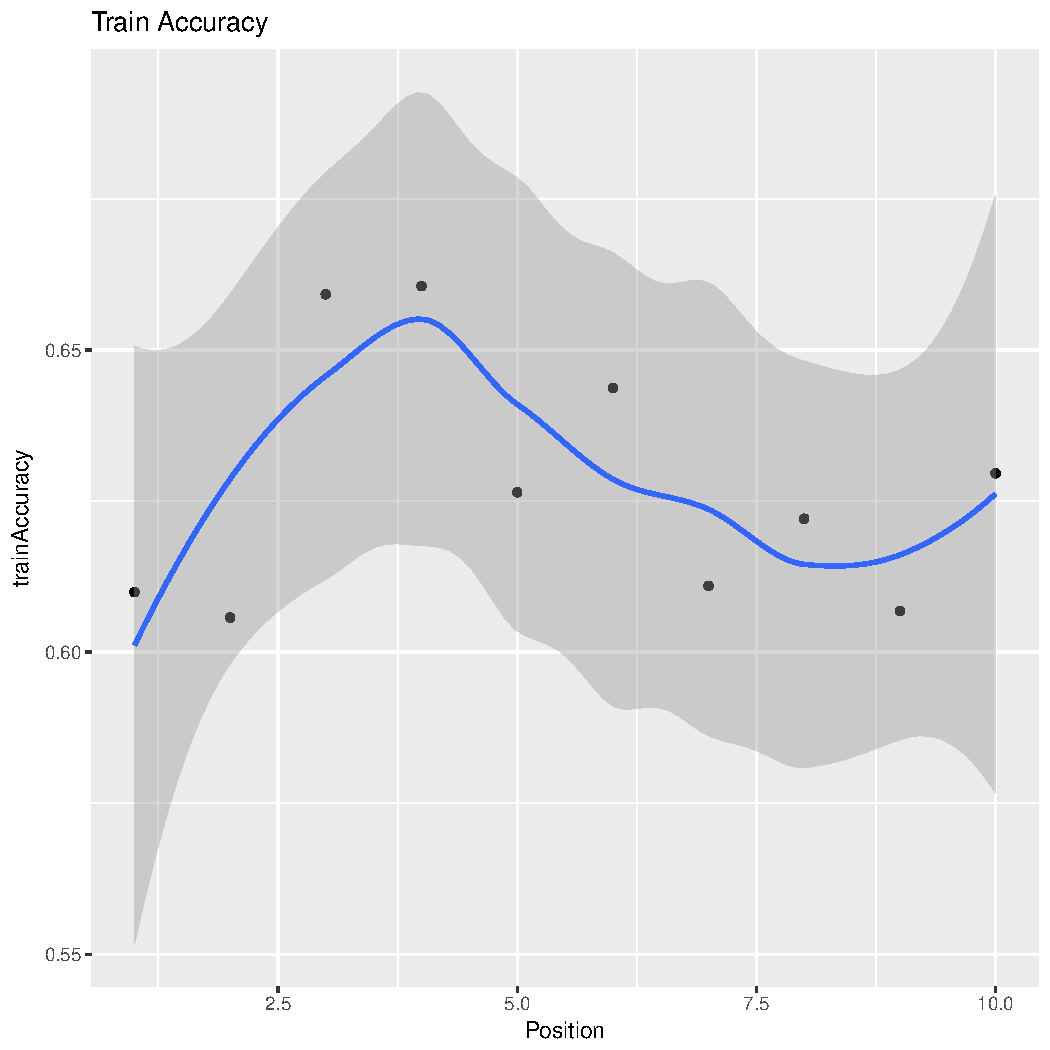
\includegraphics[width=\maxwidth]{figure/unnamed-chunk-35-4} 
\begin{kframe}

{\ttfamily\noindent\itshape\color{messagecolor}{\#\# `geom\_smooth()` using method = 'loess'}}\end{kframe}
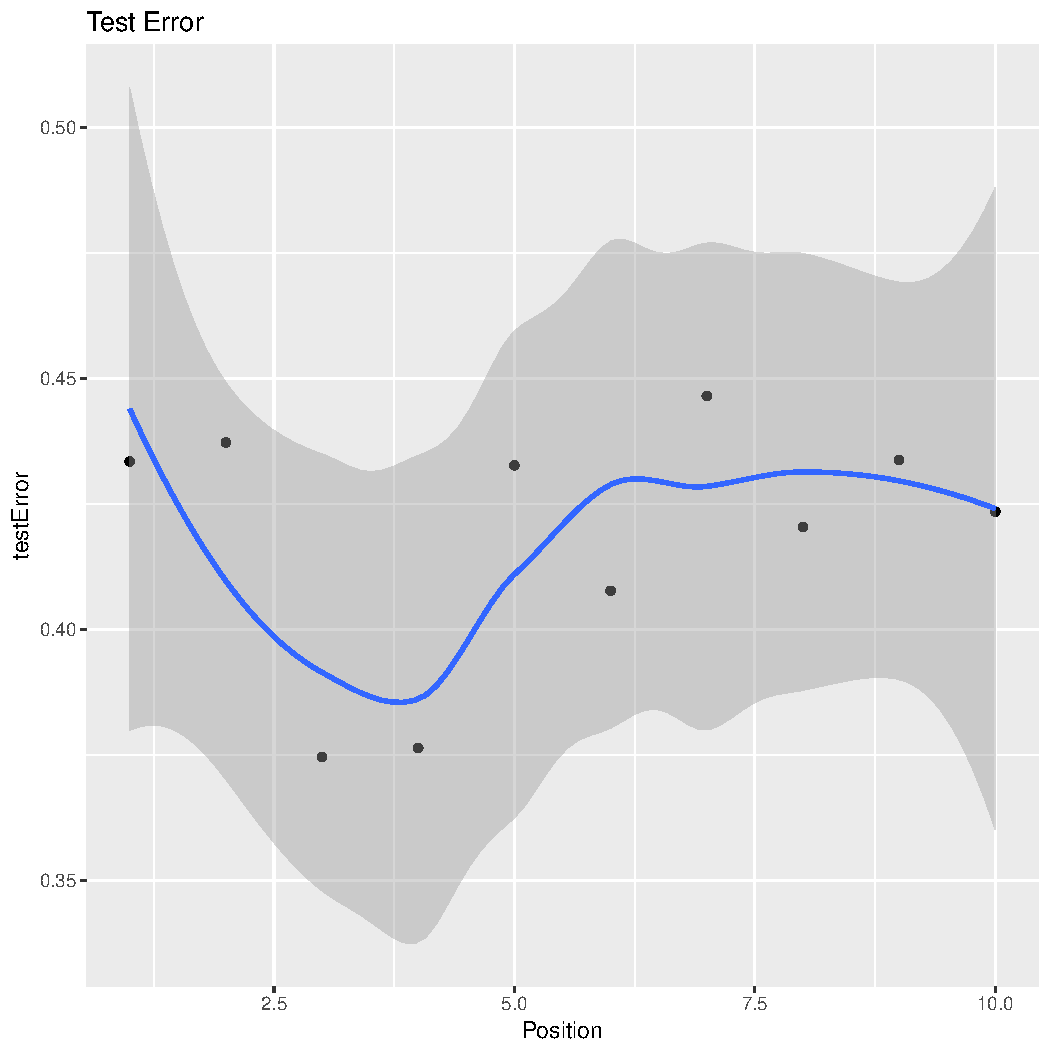
\includegraphics[width=\maxwidth]{figure/unnamed-chunk-35-5} 
\begin{kframe}

{\ttfamily\noindent\itshape\color{messagecolor}{\#\# `geom\_smooth()` using method = 'loess'}}\end{kframe}
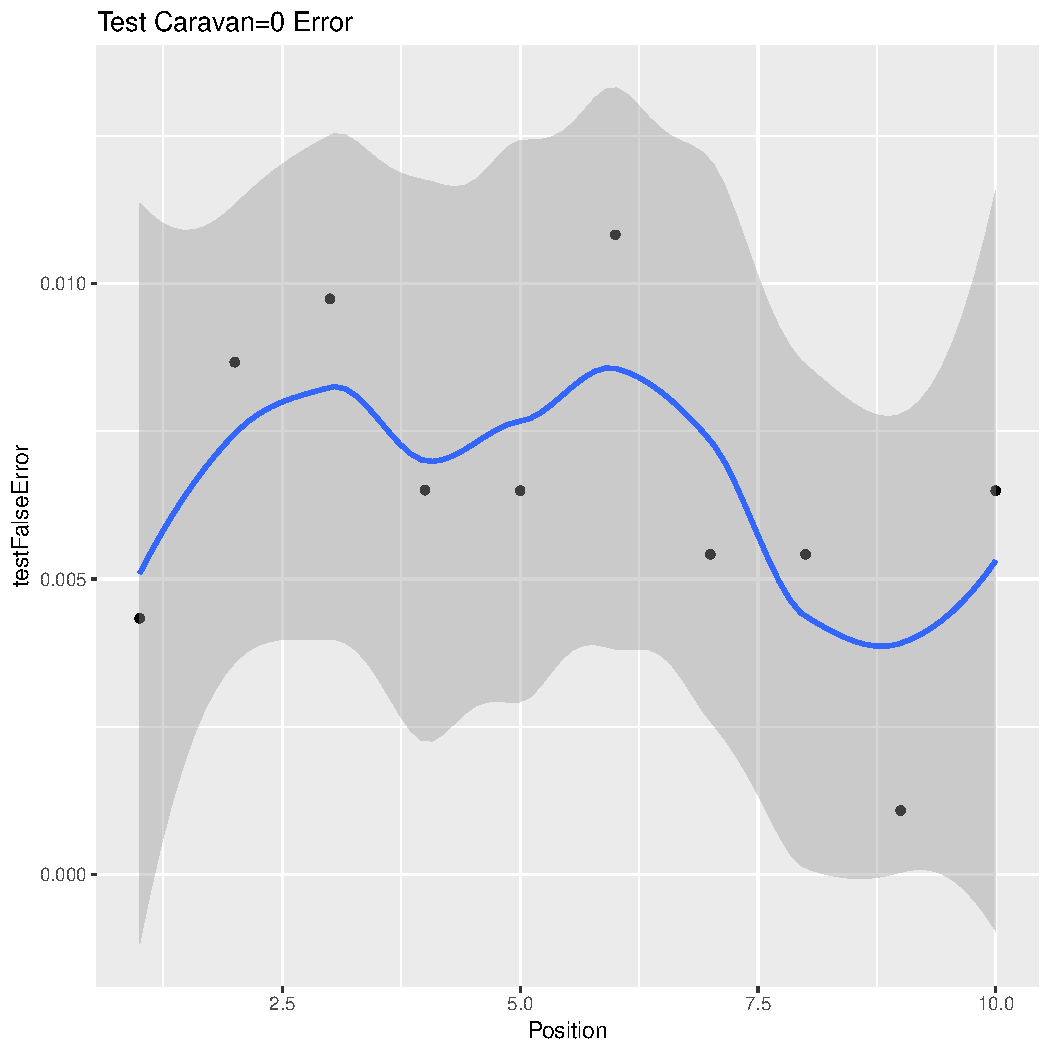
\includegraphics[width=\maxwidth]{figure/unnamed-chunk-35-6} 
\begin{kframe}

{\ttfamily\noindent\itshape\color{messagecolor}{\#\# `geom\_smooth()` using method = 'loess'}}\end{kframe}
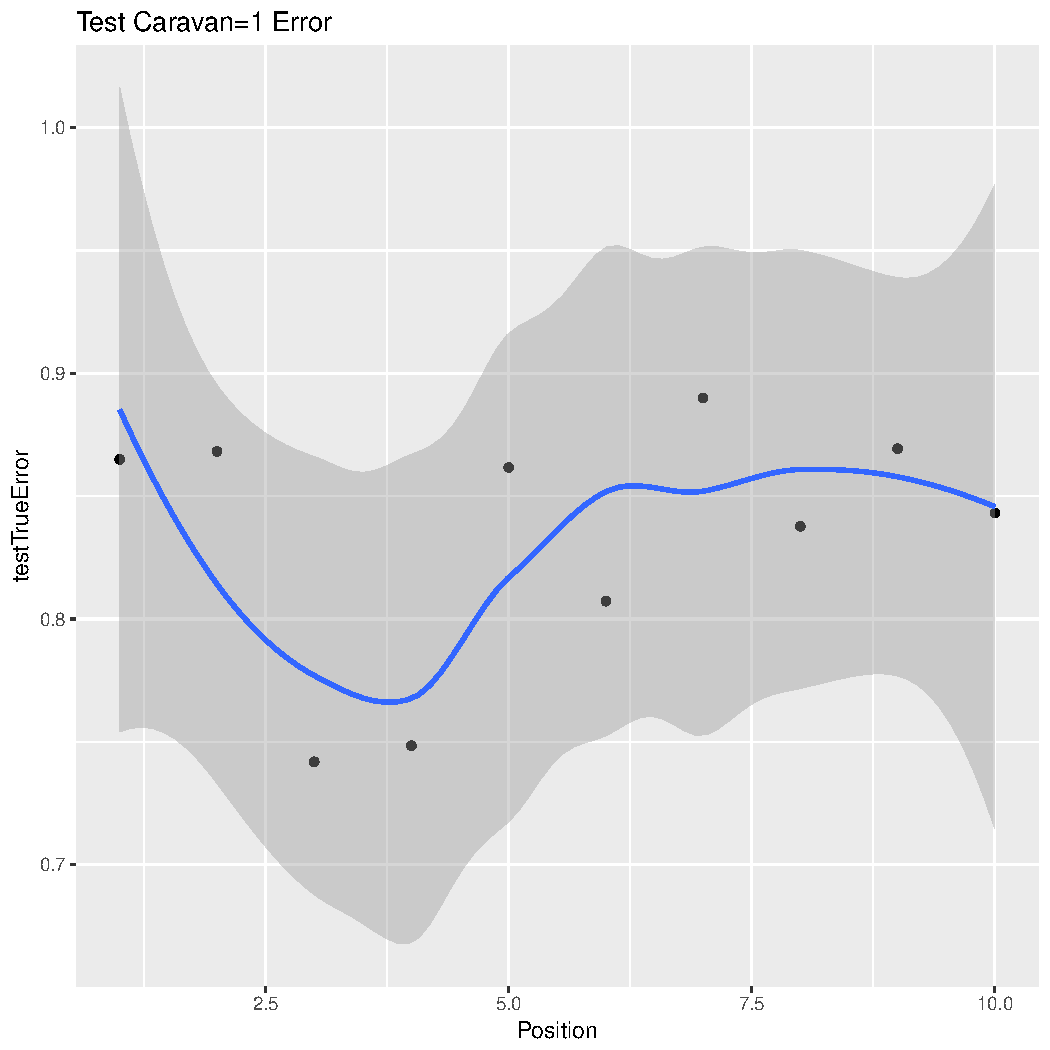
\includegraphics[width=\maxwidth]{figure/unnamed-chunk-35-7} 
\begin{kframe}

{\ttfamily\noindent\itshape\color{messagecolor}{\#\# `geom\_smooth()` using method = 'loess'}}\end{kframe}
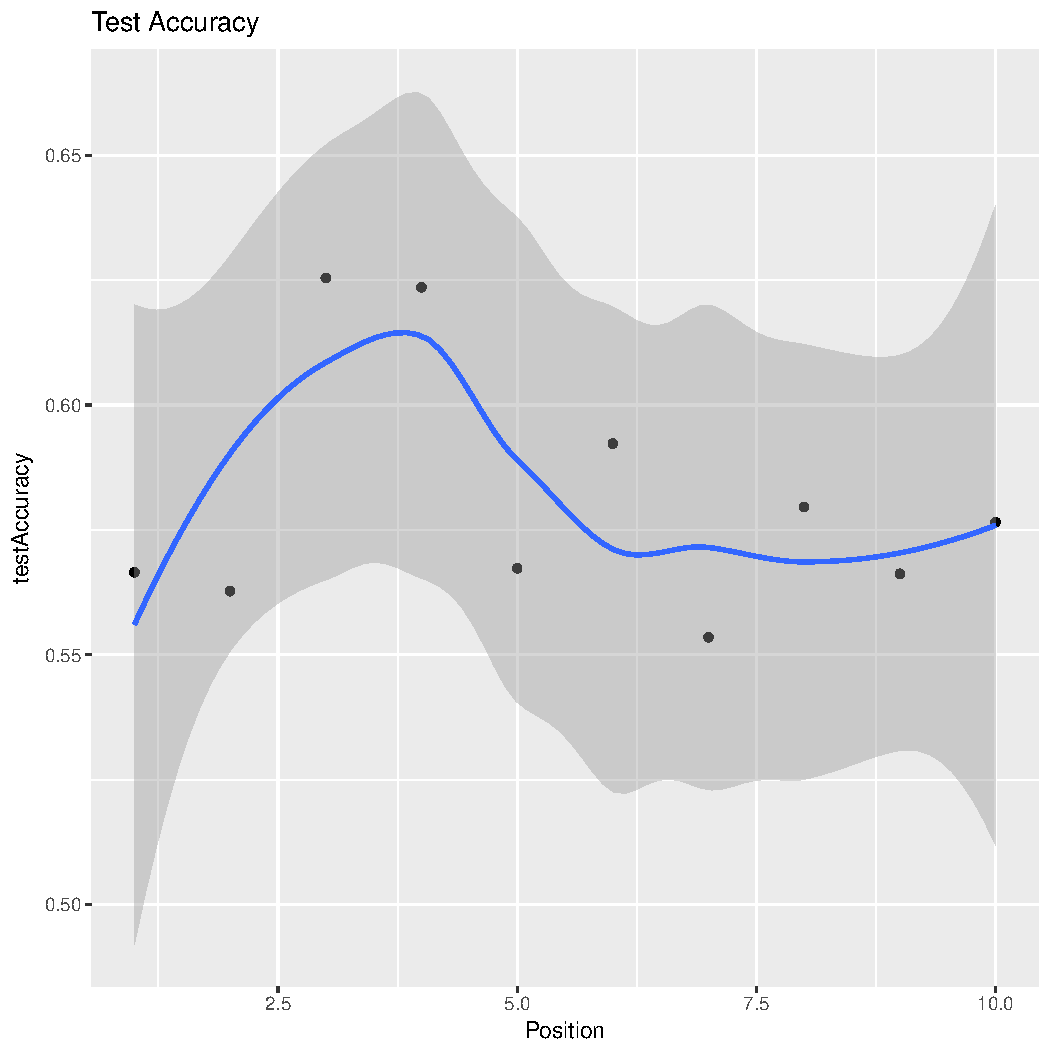
\includegraphics[width=\maxwidth]{figure/unnamed-chunk-35-8} 
\begin{kframe}\begin{verbatim}
## [1] "Average OOB: 0.372446356551945"
## [1] "Average CARAVAN=0 Error: 0.0143427448828463"
## [1] "Average CARAVAN=1 Error: 0.732710328839835"
## [1] "Average Train Accuracy: 0.62748983764441"
## [1] " "
## [1] "Average Test Error: 0.418627256701469"
## [1] "Average CARAVAN=0 Error: 0.00649678959538114"
## [1] "Average CARAVAN=1 Error: 0.83322440087146"
## [1] "Average Test Accuracy: 0.581372743298531"
\end{verbatim}
\end{kframe}
\end{knitrout}
During testing, the changes caused a greater range in test errors and accuracies. Values now varied greatly. Train errors were increased slighly but test errors were improved slightly also. Change was roughly 1 percent in each case. Error rates for CARAVAN=1 increased also and were near 90 percent again. 

I will not try and fine tune the randomForest function variable nodesize. I will write a function to do this that works in a similar way to the function I wrote to test ntrees. Nodesize in this case refers to the minimum number of terminal nodes. By default for classification this is set to 1. This is very low and will create very large trees. I hope to increase the accuracy and decrease modeling times by varying this. 
\begin{knitrout}
\definecolor{shadecolor}{rgb}{0.969, 0.969, 0.969}\color{fgcolor}\begin{kframe}
\begin{alltt}
\hlcom{#Tweek Nodesize}
\hlstd{testNodeSize} \hlkwb{<-} \hlkwa{function}\hlstd{(}\hlkwc{trainData}\hlstd{,}\hlkwc{testData}\hlstd{,}\hlkwc{ntrees}\hlstd{)\{}
  \hlstd{nsize}\hlkwb{<-}\hlnum{0}
  \hlstd{results}\hlkwb{<-}\hlkwd{data.frame}\hlstd{(}\hlkwc{Nodesize}\hlstd{=}\hlkwd{as.numeric}\hlstd{(),}
                      \hlkwc{OOB}\hlstd{=}\hlkwd{as.numeric}\hlstd{(),}
                      \hlkwc{trainFalseError}\hlstd{=}\hlkwd{as.numeric}\hlstd{(),}
                      \hlkwc{trainTrueError}\hlstd{=}\hlkwd{as.numeric}\hlstd{(),}
                      \hlkwc{testError}\hlstd{=}\hlkwd{as.numeric}\hlstd{(),}
                      \hlkwc{testFalseError}\hlstd{=}\hlkwd{as.numeric}\hlstd{(),}
                      \hlkwc{testTrueError}\hlstd{=}\hlkwd{as.numeric}\hlstd{(),}
                      \hlkwc{trainAccuracy}\hlstd{=}\hlkwd{as.numeric}\hlstd{(),}
                      \hlkwc{testAccuracy}\hlstd{=}\hlkwd{as.numeric}\hlstd{())}
  \hlkwa{for} \hlstd{(i} \hlkwa{in} \hlnum{1}\hlopt{:}\hlkwd{floor}\hlstd{(}\hlkwd{nrow}\hlstd{(trainData)}\hlopt{/}\hlnum{100}\hlstd{))\{}
    \hlstd{model}\hlkwb{<-}\hlkwd{randomForest}\hlstd{(trainData[,}\hlopt{-}\hlkwd{ncol}\hlstd{(trainData)],}
                        \hlstd{trainData[,}\hlkwd{ncol}\hlstd{(trainData)],}
                        \hlkwc{xtest}\hlstd{=testData[,}\hlopt{-}\hlkwd{ncol}\hlstd{(testData)],}
                        \hlkwc{ytest}\hlstd{=testData[,}\hlkwd{ncol}\hlstd{(testData)],}
                        \hlkwc{ntree}\hlstd{=ntrees,}
                        \hlkwc{proximity}\hlstd{=}\hlnum{TRUE}\hlstd{)}
    \hlcom{#TRAIN}
    \hlstd{oob}\hlkwb{<-}\hlstd{model}\hlopt{$}\hlstd{err.rate[}\hlkwd{nrow}\hlstd{(model}\hlopt{$}\hlstd{test}\hlopt{$}\hlstd{err.rate),}\hlnum{1}\hlstd{,}\hlkwc{drop}\hlstd{=}\hlnum{FALSE}\hlstd{]}
    \hlstd{trainFalse}\hlkwb{<-}\hlstd{model}\hlopt{$}\hlstd{err.rate[}\hlkwd{nrow}\hlstd{(model}\hlopt{$}\hlstd{test}\hlopt{$}\hlstd{err.rate),}\hlnum{2}\hlstd{,}\hlkwc{drop}\hlstd{=}\hlnum{FALSE}\hlstd{]}
    \hlstd{trainTrue}\hlkwb{<-}\hlstd{model}\hlopt{$}\hlstd{err.rate[}\hlkwd{nrow}\hlstd{(model}\hlopt{$}\hlstd{test}\hlopt{$}\hlstd{err.rate),}\hlnum{3}\hlstd{,}\hlkwc{drop}\hlstd{=}\hlnum{FALSE}\hlstd{]}
    \hlstd{trainAccuracy}\hlkwb{<-}\hlkwd{sum}\hlstd{(}\hlkwd{diag}\hlstd{(model}\hlopt{$}\hlstd{confusion))}\hlopt{/}\hlkwd{nrow}\hlstd{(trainData)}
    \hlcom{#TEST}
    \hlstd{testError}\hlkwb{<-}\hlstd{model}\hlopt{$}\hlstd{test}\hlopt{$}\hlstd{err.rate[}\hlkwd{nrow}\hlstd{(model}\hlopt{$}\hlstd{test}\hlopt{$}\hlstd{err.rate),}\hlnum{1}\hlstd{,}\hlkwc{drop}\hlstd{=}\hlnum{FALSE}\hlstd{]}
    \hlstd{testFalse}\hlkwb{<-}\hlstd{model}\hlopt{$}\hlstd{test}\hlopt{$}\hlstd{err.rate[}\hlkwd{nrow}\hlstd{(model}\hlopt{$}\hlstd{test}\hlopt{$}\hlstd{err.rate),}\hlnum{2}\hlstd{,}\hlkwc{drop}\hlstd{=}\hlnum{FALSE}\hlstd{]}
    \hlstd{testTrue}\hlkwb{<-}\hlstd{model}\hlopt{$}\hlstd{test}\hlopt{$}\hlstd{err.rate[}\hlkwd{nrow}\hlstd{(model}\hlopt{$}\hlstd{test}\hlopt{$}\hlstd{err.rate),}\hlnum{3}\hlstd{,}\hlkwc{drop}\hlstd{=}\hlnum{FALSE}\hlstd{]}
    \hlstd{testAccuracy}\hlkwb{<-}\hlkwd{sum}\hlstd{(}\hlkwd{diag}\hlstd{(model}\hlopt{$}\hlstd{test}\hlopt{$}\hlstd{confusion))}\hlopt{/}\hlkwd{nrow}\hlstd{(testData)}
    \hlstd{results[}\hlkwd{nrow}\hlstd{(results)}\hlopt{+}\hlnum{1}\hlstd{,]}\hlkwb{<-}\hlkwd{c}\hlstd{(nsize,}
                                 \hlstd{oob,}
                                 \hlstd{trainFalse,}
                                 \hlstd{trainTrue,}
                                 \hlstd{testError,}
                                 \hlstd{testFalse,}
                                 \hlstd{testTrue,}
                                 \hlstd{trainAccuracy,}
                                 \hlstd{testAccuracy)}
    \hlstd{nsize}\hlkwb{<-}\hlstd{nsize}\hlopt{+}\hlnum{1}
  \hlstd{\}}
  \hlcom{#Return node size }
  \hlstd{nodeSize}\hlkwb{<-}\hlstd{results}\hlopt{$}\hlstd{Nodesize[}\hlkwd{which.max}\hlstd{(results}\hlopt{$}\hlstd{testAccuracy)]}
  \hlkwd{return}\hlstd{(nodeSize)}
\hlstd{\}}
\end{alltt}
\end{kframe}
\end{knitrout}

I will now use the function to find nodesize.
\begin{knitrout}
\definecolor{shadecolor}{rgb}{0.969, 0.969, 0.969}\color{fgcolor}\begin{kframe}
\begin{alltt}
\hlcom{#Get node size}
\hlstd{nodeSize}\hlkwb{<-}\hlkwd{testNodeSize}\hlstd{(train,test,ntrees)}
\hlstd{nodeSize}
\end{alltt}
\begin{verbatim}
## [1] 24
\end{verbatim}
\end{kframe}
\end{knitrout}
During testing, the values for nodeSize where in the low 100s. Train and test error rates have improved. 

I will now test the accuracy of my new model, with the new values for ntree and nodesize.
\begin{knitrout}
\definecolor{shadecolor}{rgb}{0.969, 0.969, 0.969}\color{fgcolor}\begin{kframe}
\begin{alltt}
\hlcom{#Build second model with new ntree and nodesize}
\hlstd{model3}\hlkwb{<-}\hlkwd{buildModel}\hlstd{(train,test,}\hlkwc{ntrees}\hlstd{=ntrees,}\hlkwc{nodeSize}\hlstd{=nodeSize)}
\hlcom{#Display Values}
\hlkwd{displayResultsFromModel}\hlstd{(model3,}\hlkwd{nrow}\hlstd{(train),}\hlkwd{nrow}\hlstd{(test))}
\end{alltt}
\begin{verbatim}
## [1] "TRAIN"
## [1] "Train OOB Error: 0.358029480217223"
## [1] "Train CARAVAN=0 Error: 0.0244430693069307"
## [1] "Train CARAVAN=1 Error: 0.693588546529723"
## [1] "Train Accuracy: 0.641920719882088"
## [1] " "
## [1] "TEST"
## [1] "Test Error: 0.38848660391021"
## [1] "Test CARAVAN=0 Error: 0.0137184115523466"
## [1] "Test CARAVAN=1 Error: 0.765432098765432"
## [1] "Test Accuracy: 0.61151339608979"
\end{verbatim}
\begin{alltt}
\hlcom{#Plot Results}
\end{alltt}
\end{kframe}
\end{knitrout}
I will now validate the new model
\begin{knitrout}
\definecolor{shadecolor}{rgb}{0.969, 0.969, 0.969}\color{fgcolor}\begin{kframe}
\begin{alltt}
\hlcom{#Validate second model, 10 fold cross validation }
\hlstd{validateResults3}\hlkwb{<-}\hlkwd{validateModel}\hlstd{(df,ntrees,nodeSize)}
\hlkwd{displayResults}\hlstd{(validateResults3)}
\end{alltt}


{\ttfamily\noindent\itshape\color{messagecolor}{\#\# `geom\_smooth()` using method = 'loess'}}\end{kframe}
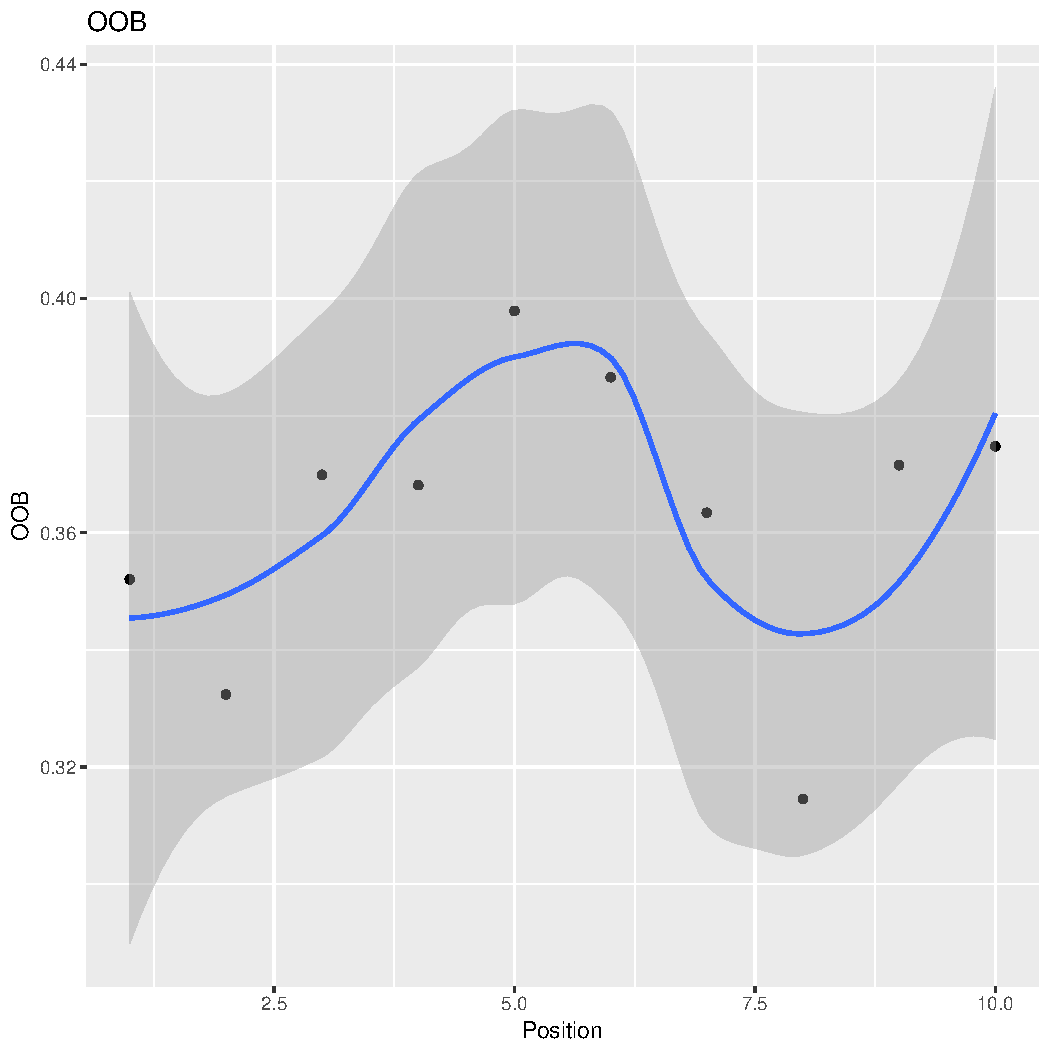
\includegraphics[width=\maxwidth]{figure/unnamed-chunk-39-1} 
\begin{kframe}

{\ttfamily\noindent\itshape\color{messagecolor}{\#\# `geom\_smooth()` using method = 'loess'}}\end{kframe}
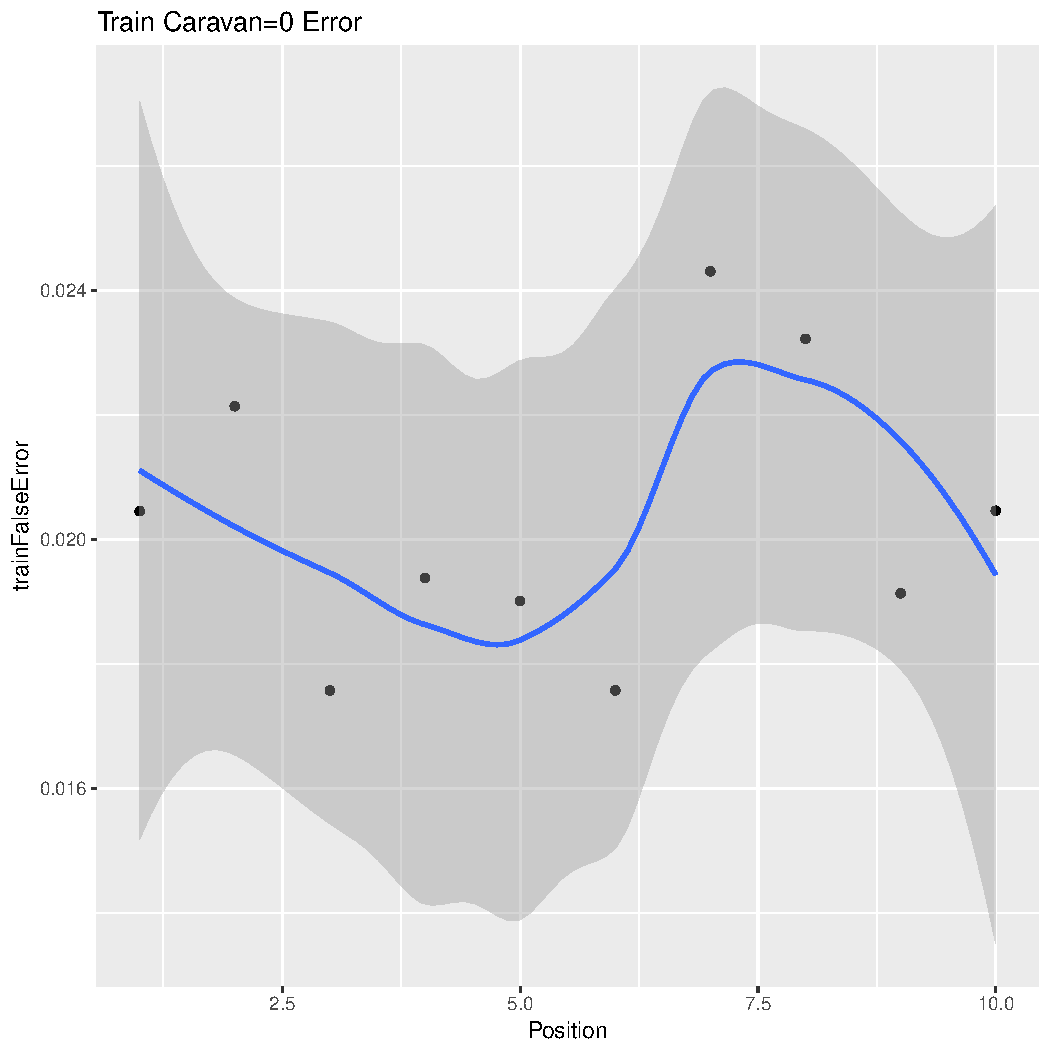
\includegraphics[width=\maxwidth]{figure/unnamed-chunk-39-2} 
\begin{kframe}

{\ttfamily\noindent\itshape\color{messagecolor}{\#\# `geom\_smooth()` using method = 'loess'}}\end{kframe}
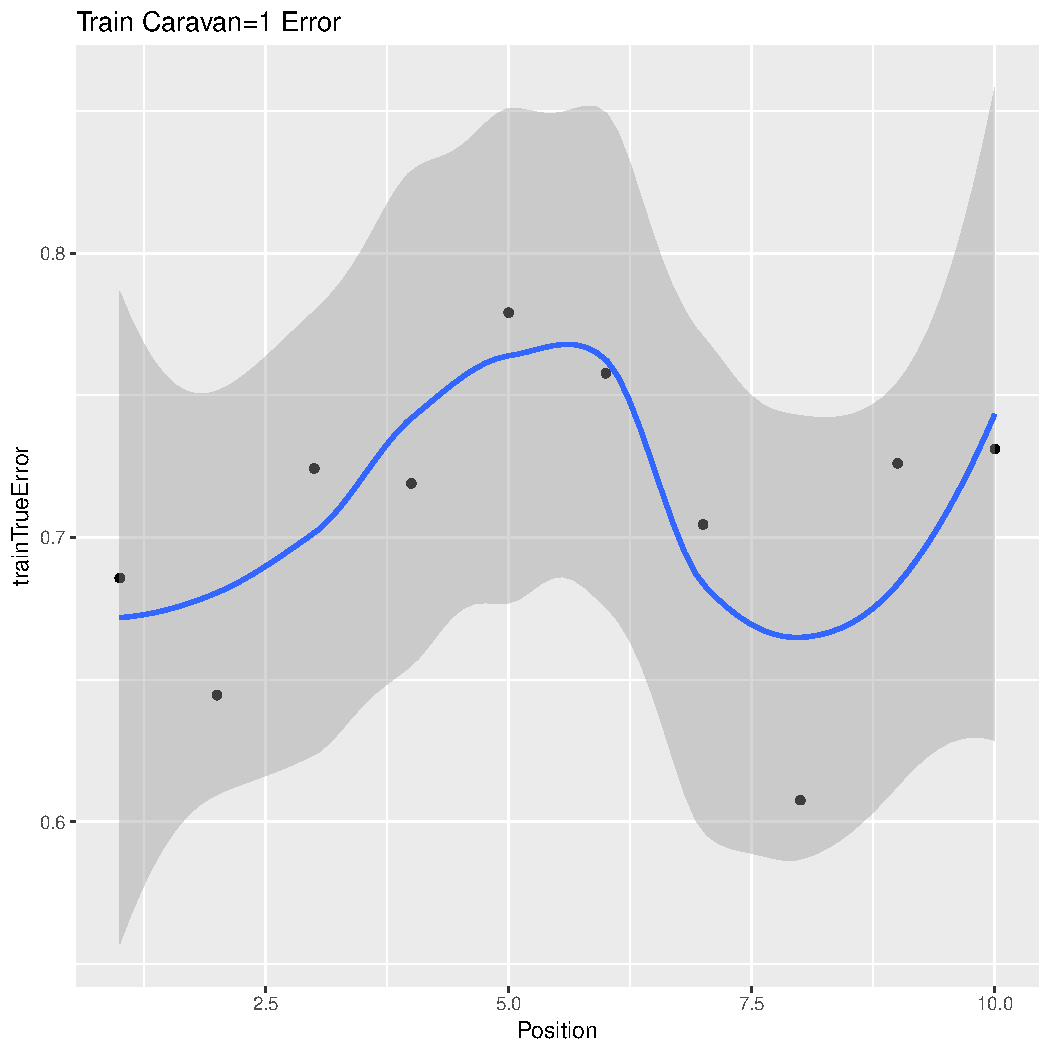
\includegraphics[width=\maxwidth]{figure/unnamed-chunk-39-3} 
\begin{kframe}

{\ttfamily\noindent\itshape\color{messagecolor}{\#\# `geom\_smooth()` using method = 'loess'}}\end{kframe}
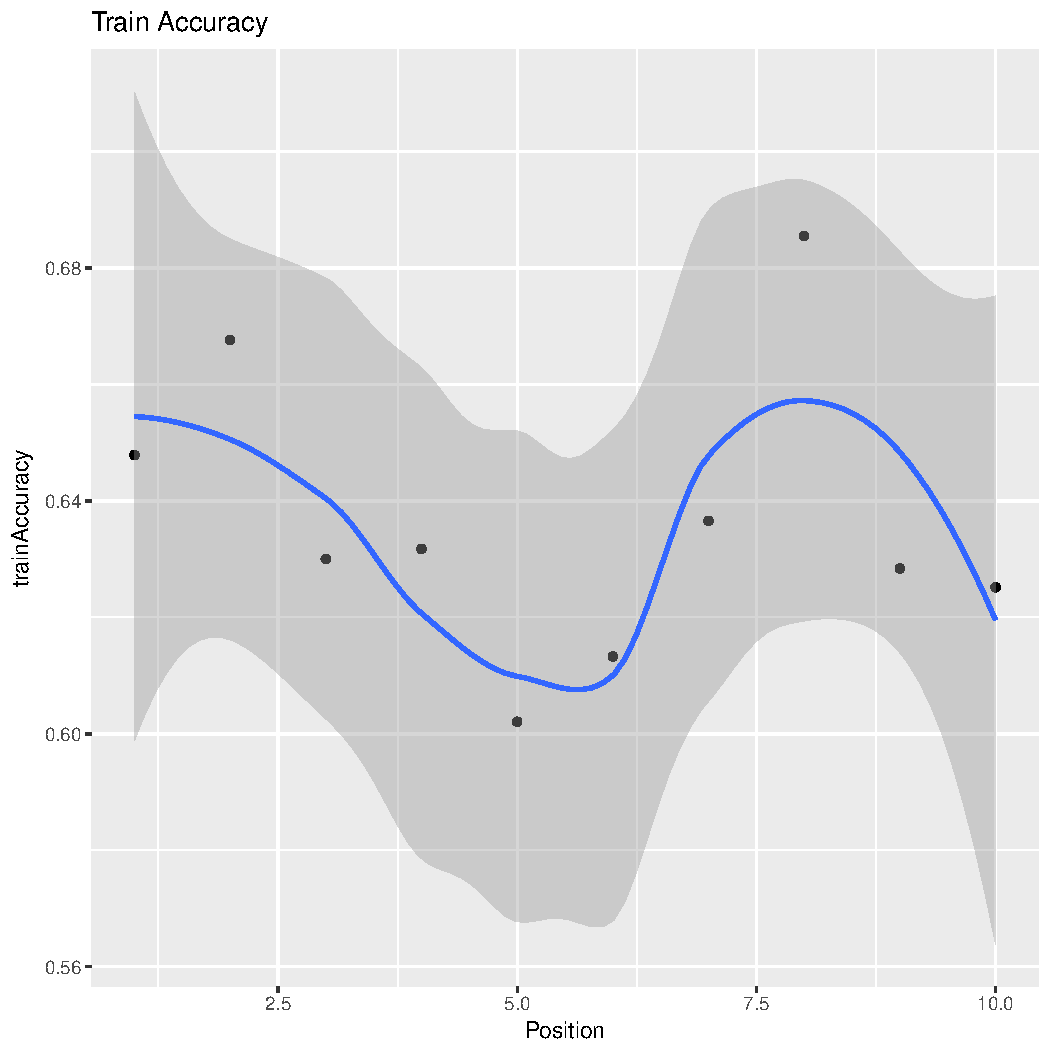
\includegraphics[width=\maxwidth]{figure/unnamed-chunk-39-4} 
\begin{kframe}

{\ttfamily\noindent\itshape\color{messagecolor}{\#\# `geom\_smooth()` using method = 'loess'}}\end{kframe}
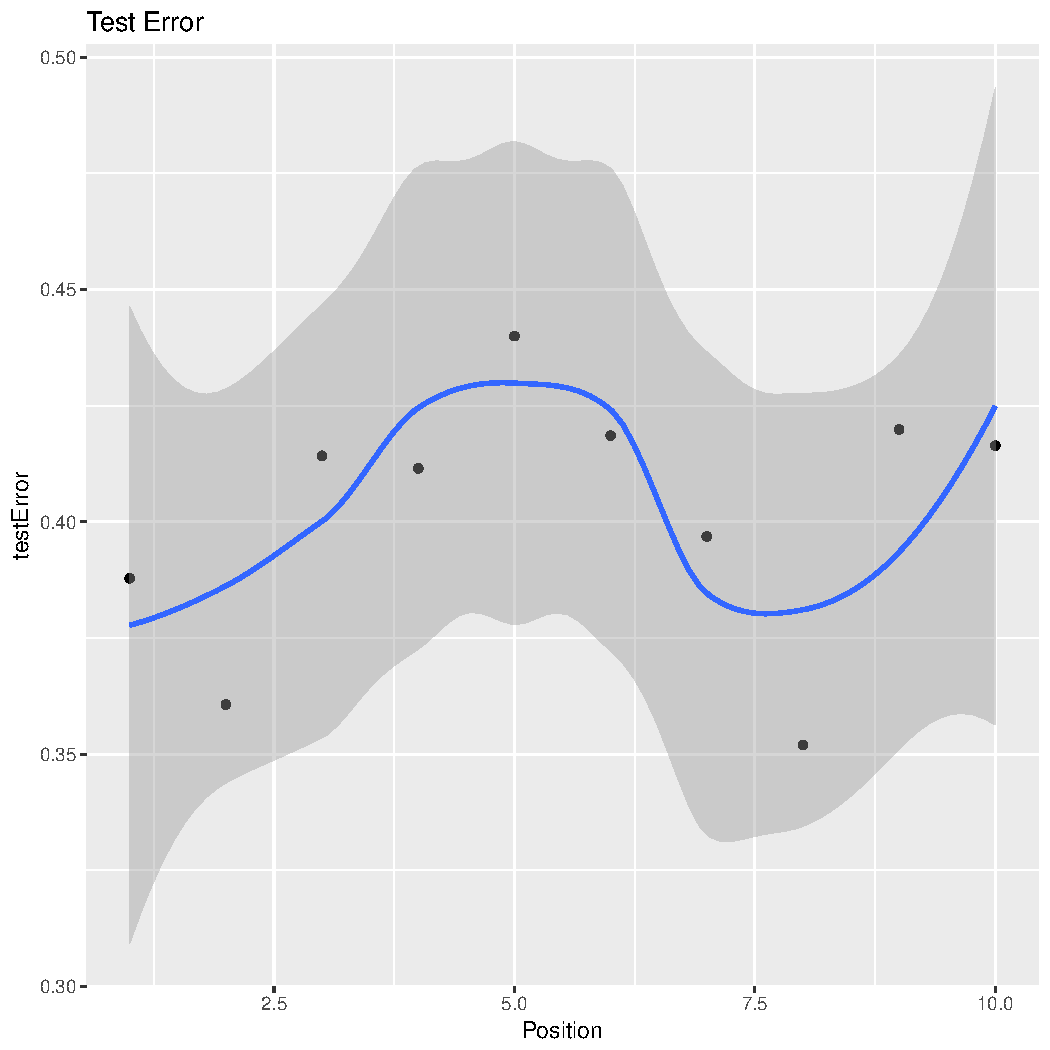
\includegraphics[width=\maxwidth]{figure/unnamed-chunk-39-5} 
\begin{kframe}

{\ttfamily\noindent\itshape\color{messagecolor}{\#\# `geom\_smooth()` using method = 'loess'}}\end{kframe}
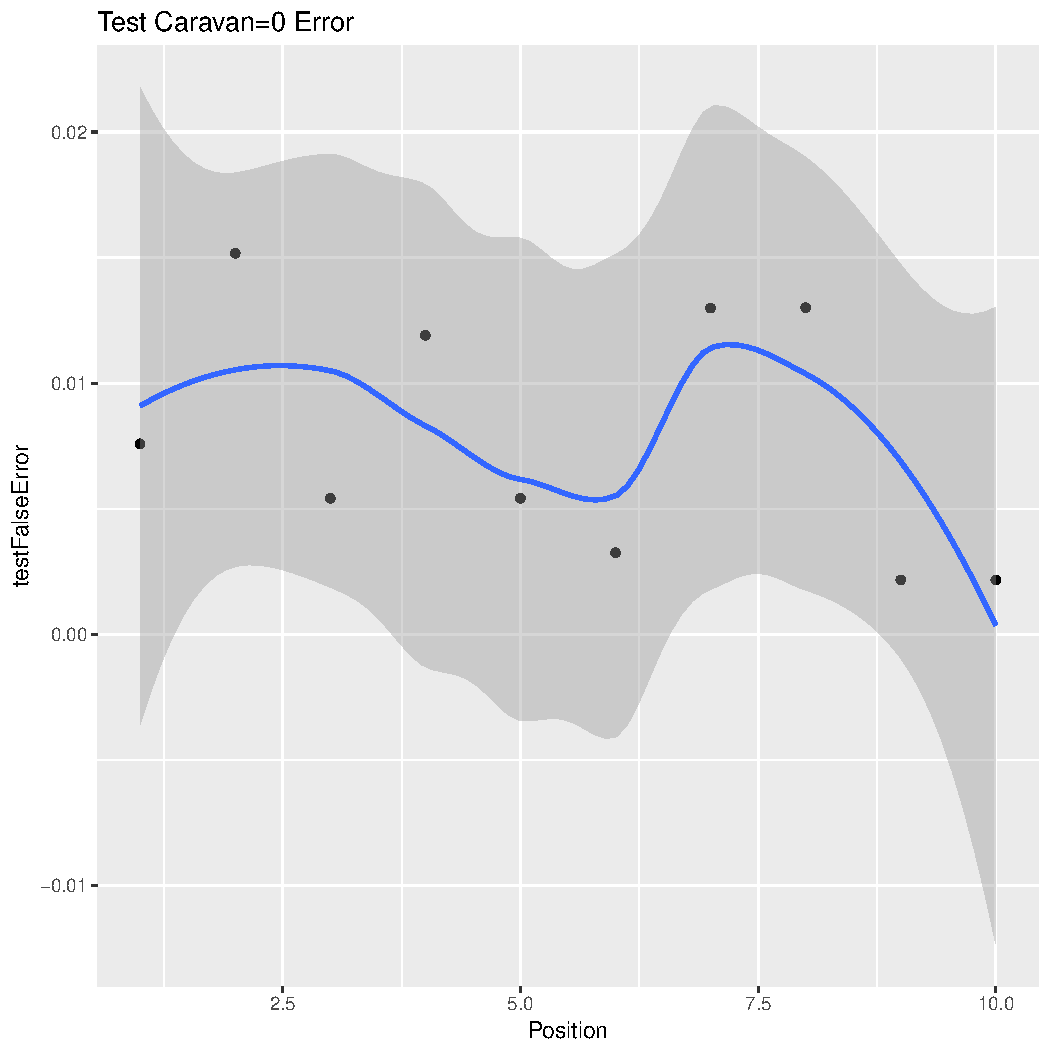
\includegraphics[width=\maxwidth]{figure/unnamed-chunk-39-6} 
\begin{kframe}

{\ttfamily\noindent\itshape\color{messagecolor}{\#\# `geom\_smooth()` using method = 'loess'}}\end{kframe}
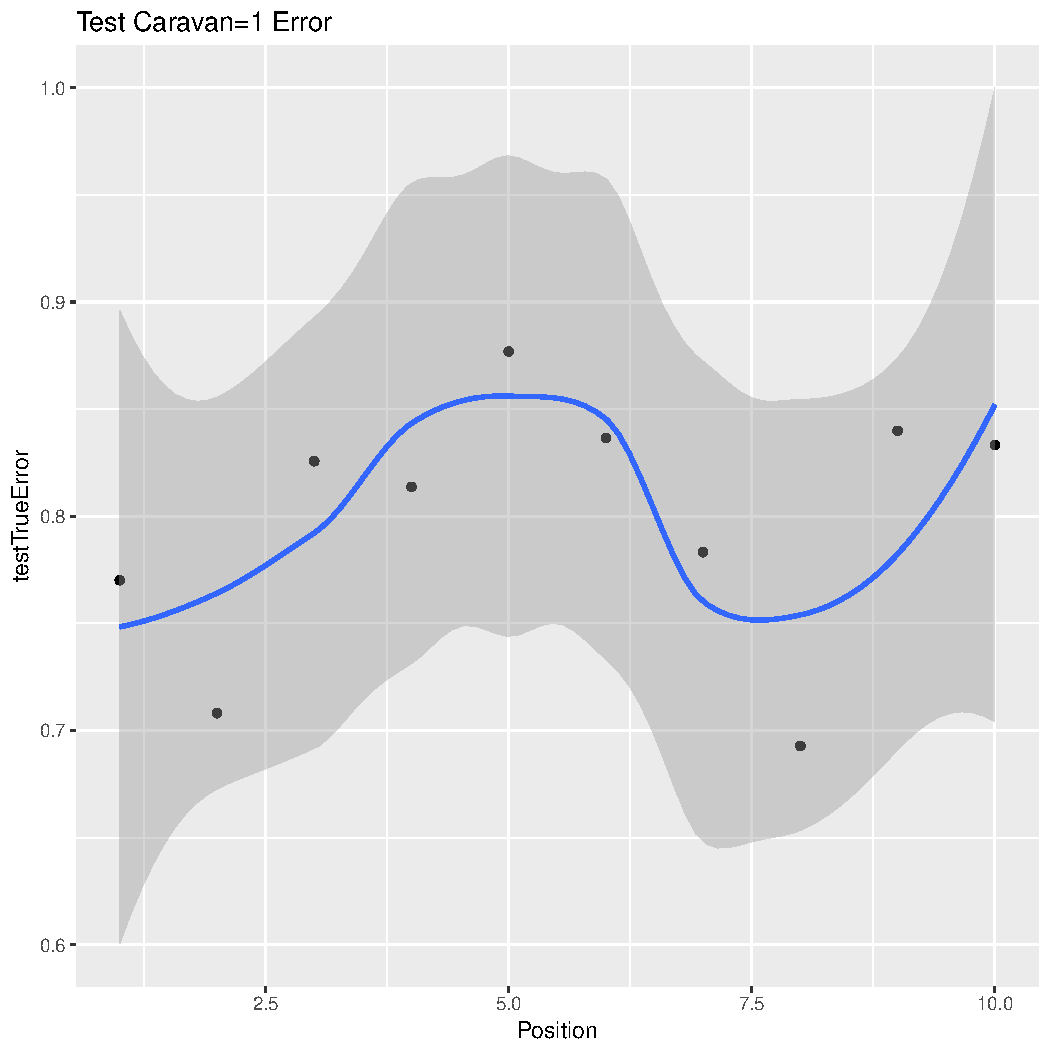
\includegraphics[width=\maxwidth]{figure/unnamed-chunk-39-7} 
\begin{kframe}

{\ttfamily\noindent\itshape\color{messagecolor}{\#\# `geom\_smooth()` using method = 'loess'}}\end{kframe}
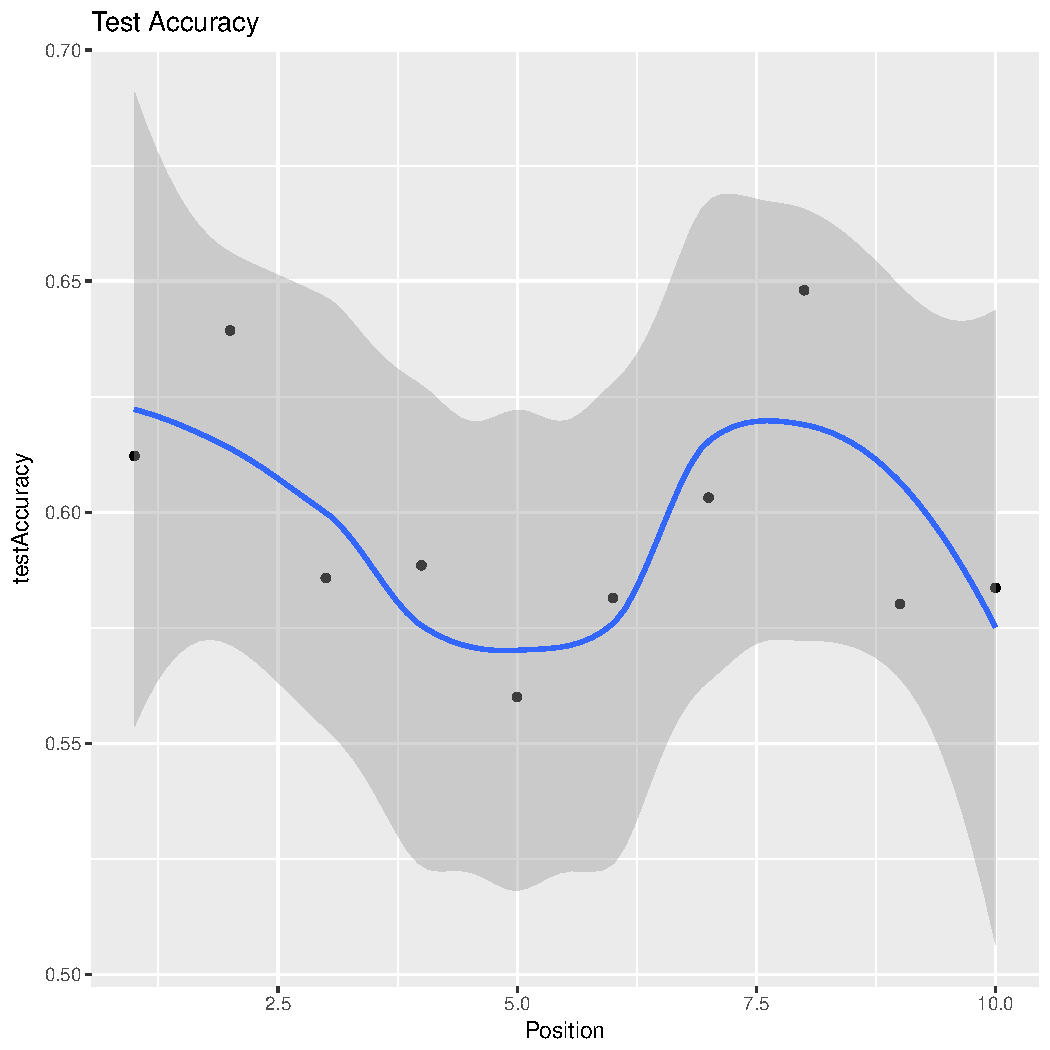
\includegraphics[width=\maxwidth]{figure/unnamed-chunk-39-8} 
\begin{kframe}\begin{verbatim}
## [1] "Average OOB: 0.36311377977941"
## [1] "Average CARAVAN=0 Error: 0.0203225571676887"
## [1] "Average CARAVAN=1 Error: 0.707970966236665"
## [1] "Average Train Accuracy: 0.636829593635163"
## [1] " "
## [1] "Average Test Error: 0.401789378264775"
## [1] "Average CARAVAN=0 Error: 0.00790512304596812"
## [1] "Average CARAVAN=1 Error: 0.798039215686275"
## [1] "Average Test Accuracy: 0.598210621735225"
\end{verbatim}
\end{kframe}
\end{knitrout}
Error rates and accuracies have improved. Train accuracy is not in the high 50s low 60 range. Same for test accruacy. Train accuracy is still higher than test accuracy. The biggest imporovement is in the error rate for when CARAVAN = 1. Error rates are now in mid 60s low 70s range. This still isn't great but Is a good improvement over the original model. Error rates for when CARAVAN=0 however have also increased by around 1-2 percent. This isn't a huge increase and was worth the drop in the error rates for CARAVAN=1. 

Now I will use the importance function from the randomForest package, to create plots of mean decrease in accuracy and mean decrease in Gini. I will also create a list of each ordered highest to lowest which I will use to try and remove variables which are making my model less accurate. 
\begin{knitrout}
\definecolor{shadecolor}{rgb}{0.969, 0.969, 0.969}\color{fgcolor}\begin{kframe}
\begin{alltt}
\hlcom{#Mean Decrease in accuracy}
\hlstd{meanDecreaseAccuracy}\hlkwb{<-}\hlkwd{importance}\hlstd{(model2,}\hlkwc{type}\hlstd{=}\hlnum{1}\hlstd{)}
\hlcom{#Order highest to lowest}
\hlstd{meanDecreaseAccuracy}\hlkwb{<-}\hlstd{meanDecreaseAccuracy[}\hlkwd{order}\hlstd{(}\hlopt{-}\hlstd{meanDecreaseAccuracy),,}\hlkwc{drop}\hlstd{=}\hlnum{FALSE}\hlstd{]}
\hlcom{#Plot}
\hlkwd{varImpPlot}\hlstd{(model2,}\hlkwc{type}\hlstd{=}\hlnum{1}\hlstd{)}
\end{alltt}
\end{kframe}
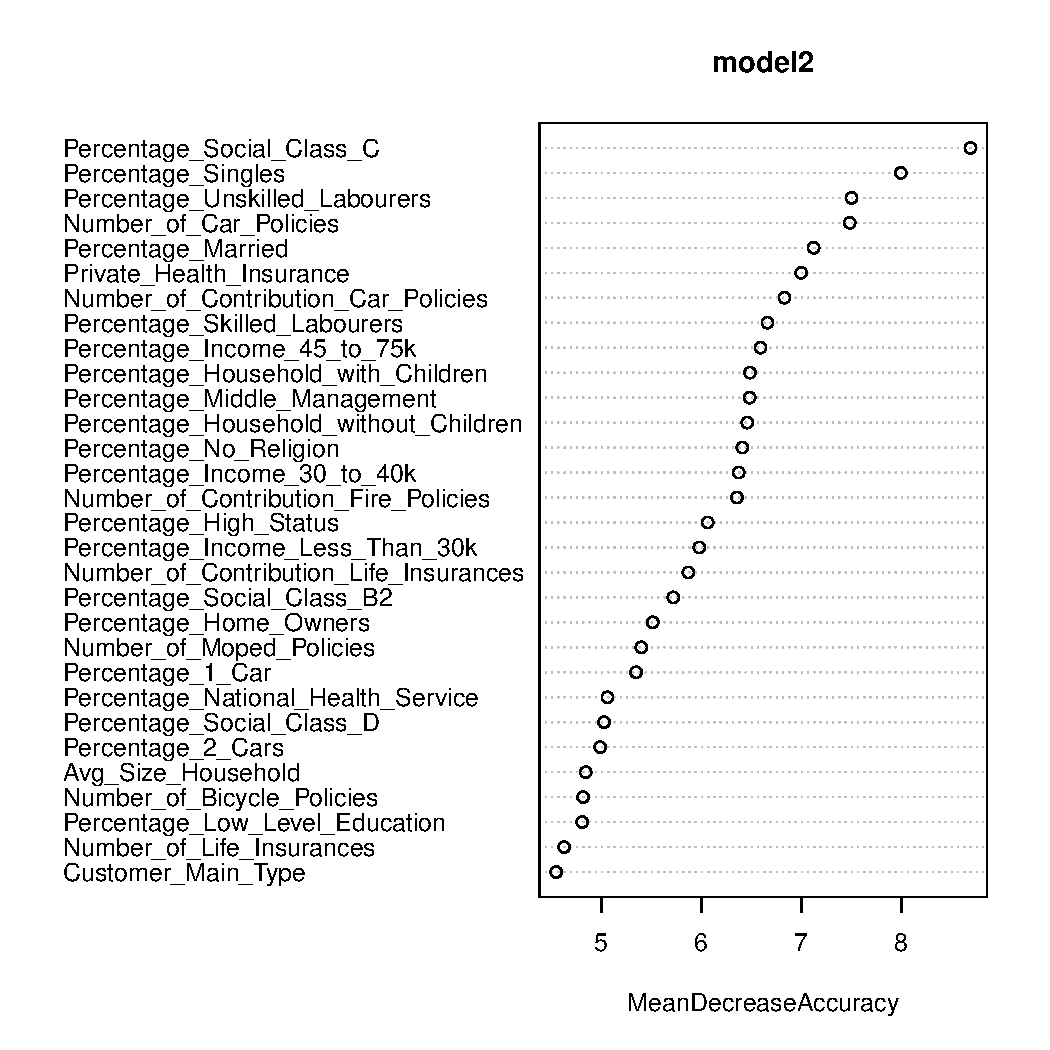
\includegraphics[width=\maxwidth]{figure/unnamed-chunk-40-1} 
\begin{kframe}\begin{alltt}
\hlcom{#Mean decrease in node impurity}
\hlstd{meanDecreaseGini}\hlkwb{<-}\hlkwd{importance}\hlstd{(model2,}\hlkwc{type}\hlstd{=}\hlnum{2}\hlstd{)}
\hlcom{#Order highest to lowest}
\hlstd{meanDecreaseGini}\hlkwb{<-}\hlstd{meanDecreaseGini[}\hlkwd{order}\hlstd{(}\hlopt{-}\hlstd{meanDecreaseGini),,}\hlkwc{drop}\hlstd{=}\hlnum{FALSE}\hlstd{]}
\hlcom{#Plot}
\hlkwd{varImpPlot}\hlstd{(model2,}\hlkwc{type}\hlstd{=}\hlnum{2}\hlstd{)}
\end{alltt}
\end{kframe}
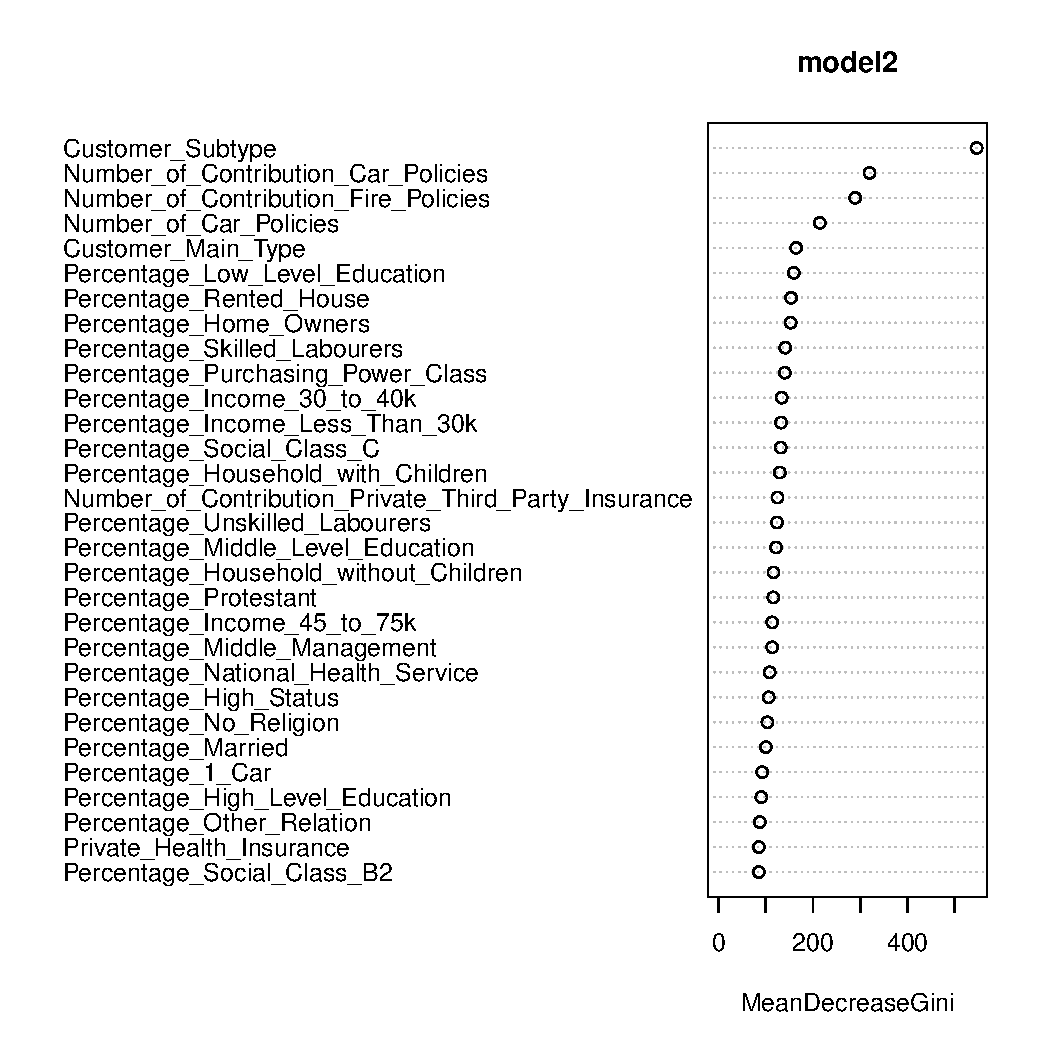
\includegraphics[width=\maxwidth]{figure/unnamed-chunk-40-2} 

\end{knitrout}
I will remove any columns that have a negative mean decrease in accuracy value(if any). I am doing this because in theory this should remove variables which are having a negative effect on the overal accuracy of the model. 
\begin{knitrout}
\definecolor{shadecolor}{rgb}{0.969, 0.969, 0.969}\color{fgcolor}\begin{kframe}
\begin{alltt}
\hlcom{#Get negative or 0 MDA}
\hlstd{cols}\hlkwb{<-}\hlkwd{rownames}\hlstd{(meanDecreaseAccuracy[meanDecreaseAccuracy}\hlopt{<}\hlnum{0}\hlstd{,,}\hlkwc{drop}\hlstd{=}\hlnum{FALSE}\hlstd{])}
\hlcom{#Show cols being removed}
\hlstd{cols}
\end{alltt}
\begin{verbatim}
## [1] "Customer_Subtype"
\end{verbatim}
\begin{alltt}
\hlcom{#Remove cols}
\hlkwa{if} \hlstd{(}\hlopt{!}\hlkwd{is.null}\hlstd{(cols))\{}
  \hlstd{df}\hlkwb{<-}\hlstd{df[,}\hlopt{!}\hlstd{(}\hlkwd{colnames}\hlstd{(df)} \hlopt \hlstd{cols)]}
  \hlstd{train}\hlkwb{<-}\hlstd{train[,}\hlopt{!}\hlstd{(}\hlkwd{colnames}\hlstd{(train)} \hlopt \hlstd{cols)]}
  \hlstd{test}\hlkwb{<-}\hlstd{test[,}\hlopt{!}\hlstd{(}\hlkwd{colnames}\hlstd{(test)} \hlopt \hlstd{cols)]}
\hlstd{\}}
\end{alltt}
\end{kframe}
\end{knitrout}
I will now test the accuracy of the final model
\begin{knitrout}
\definecolor{shadecolor}{rgb}{0.969, 0.969, 0.969}\color{fgcolor}\begin{kframe}
\begin{alltt}
\hlcom{#Build final model, with removed columns based on mean decrease in accuracy}
\hlstd{model4}\hlkwb{<-}\hlkwd{buildModel}\hlstd{(train,test,}\hlkwc{ntrees}\hlstd{=ntrees,}\hlkwc{nodeSize}\hlstd{=nodeSize)}
\hlcom{#Display values}
\hlkwd{displayResultsFromModel}\hlstd{(model4,}\hlkwd{nrow}\hlstd{(train),}\hlkwd{nrow}\hlstd{(test))}
\end{alltt}
\begin{verbatim}
## [1] "TRAIN"
## [1] "Train OOB Error: 0.0712179984484096"
## [1] "Train CARAVAN=0 Error: 0.118193069306931"
## [1] "Train CARAVAN=1 Error: 0.0239651416122004"
## [1] "Train Accuracy: 0.928709952680164"
## [1] " "
## [1] "TEST"
## [1] "Test Error: 0.0640839971035482"
## [1] "Test CARAVAN=0 Error: 0.110830324909747"
## [1] "Test CARAVAN=1 Error: 0.0170660856935367"
## [1] "Test Accuracy: 0.935916002896452"
\end{verbatim}
\begin{alltt}
\hlcom{#Plot Error}
\hlkwd{plot}\hlstd{(model4)}
\end{alltt}
\end{kframe}
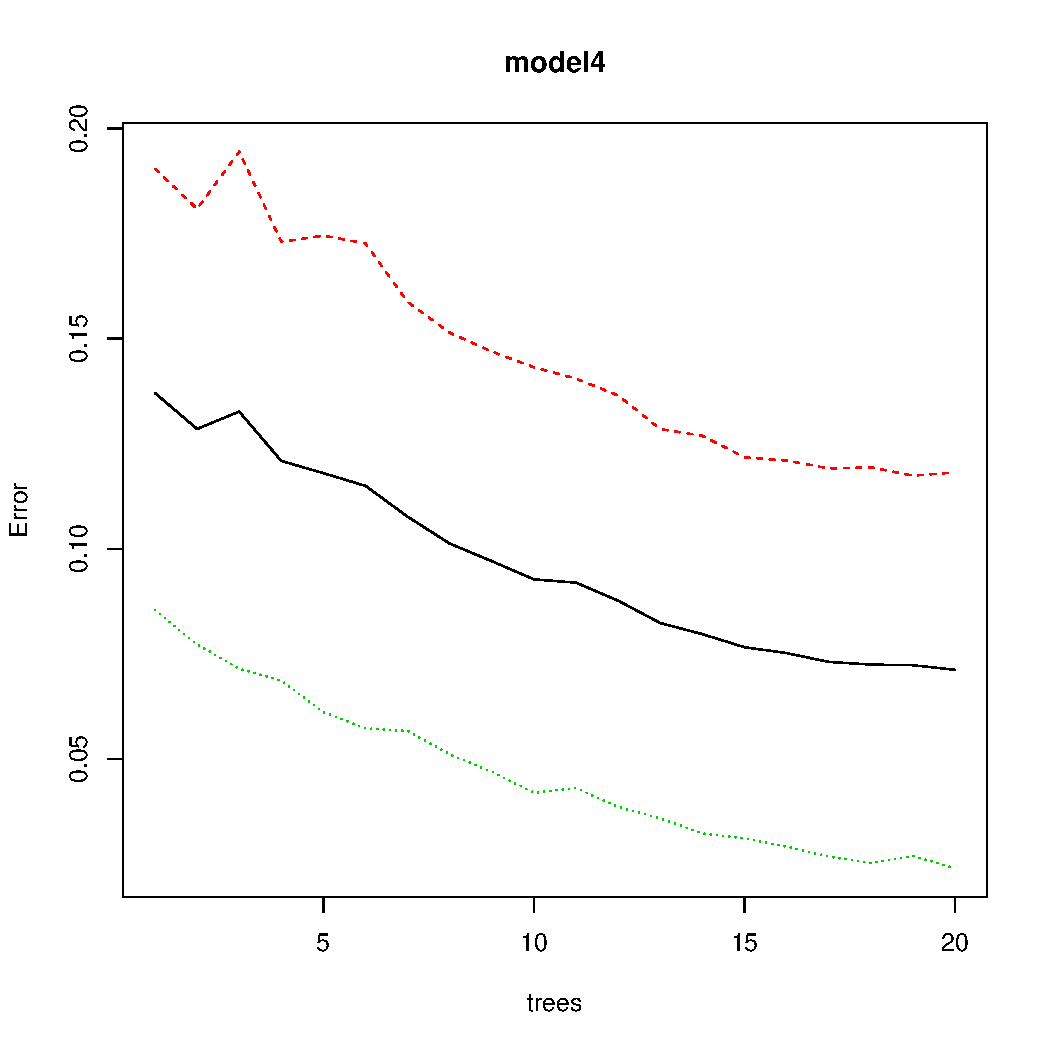
\includegraphics[width=\maxwidth]{figure/unnamed-chunk-42-1} 

\end{knitrout}

I will now validate the final model
\begin{knitrout}
\definecolor{shadecolor}{rgb}{0.969, 0.969, 0.969}\color{fgcolor}\begin{kframe}
\begin{alltt}
\hlcom{#Validate final model, 10 fold cross validation }
\hlstd{validateResults4}\hlkwb{<-}\hlkwd{validateModel}\hlstd{(df,ntrees,nodeSize)}
\hlkwd{displayResults}\hlstd{(validateResults4)}
\end{alltt}


{\ttfamily\noindent\itshape\color{messagecolor}{\#\# `geom\_smooth()` using method = 'loess'}}\end{kframe}
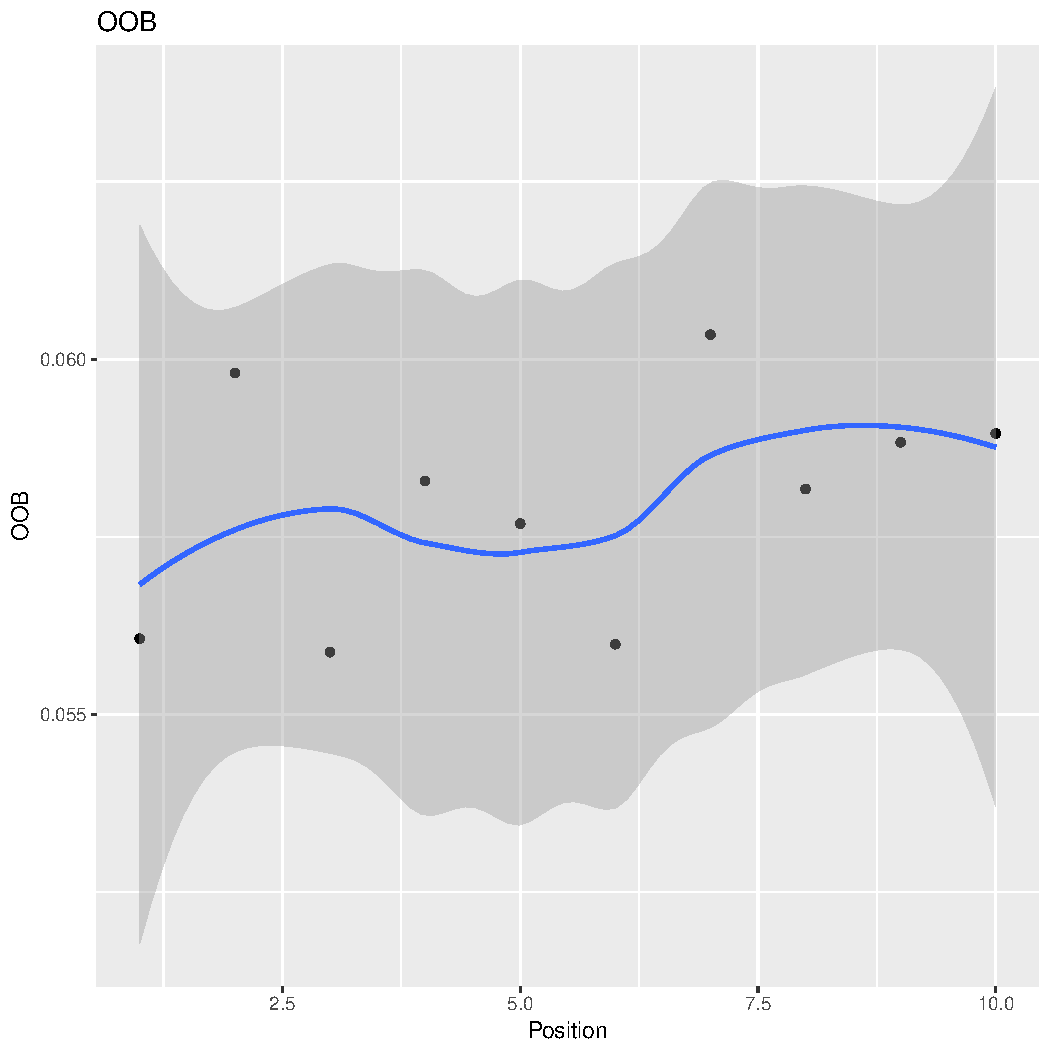
\includegraphics[width=\maxwidth]{figure/unnamed-chunk-43-1} 
\begin{kframe}

{\ttfamily\noindent\itshape\color{messagecolor}{\#\# `geom\_smooth()` using method = 'loess'}}\end{kframe}
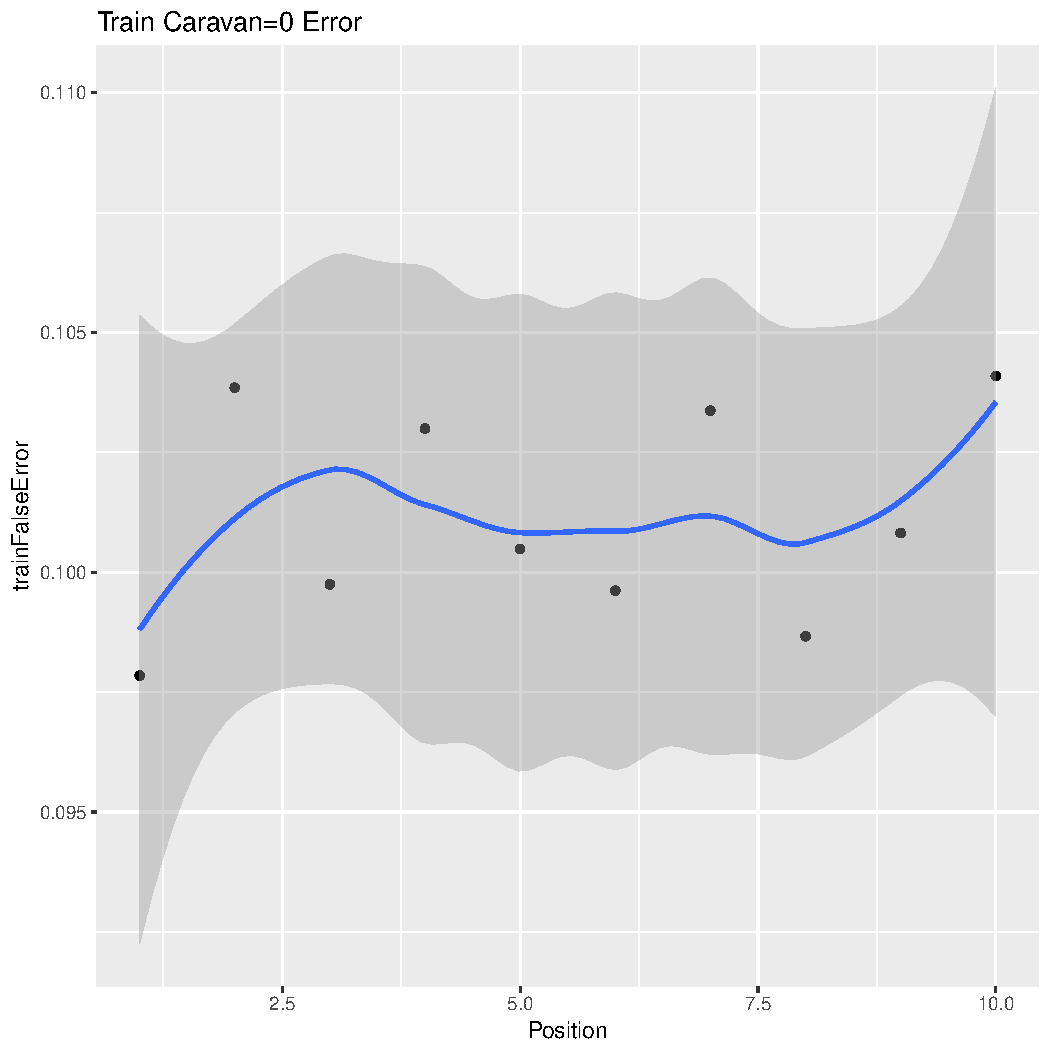
\includegraphics[width=\maxwidth]{figure/unnamed-chunk-43-2} 
\begin{kframe}

{\ttfamily\noindent\itshape\color{messagecolor}{\#\# `geom\_smooth()` using method = 'loess'}}\end{kframe}
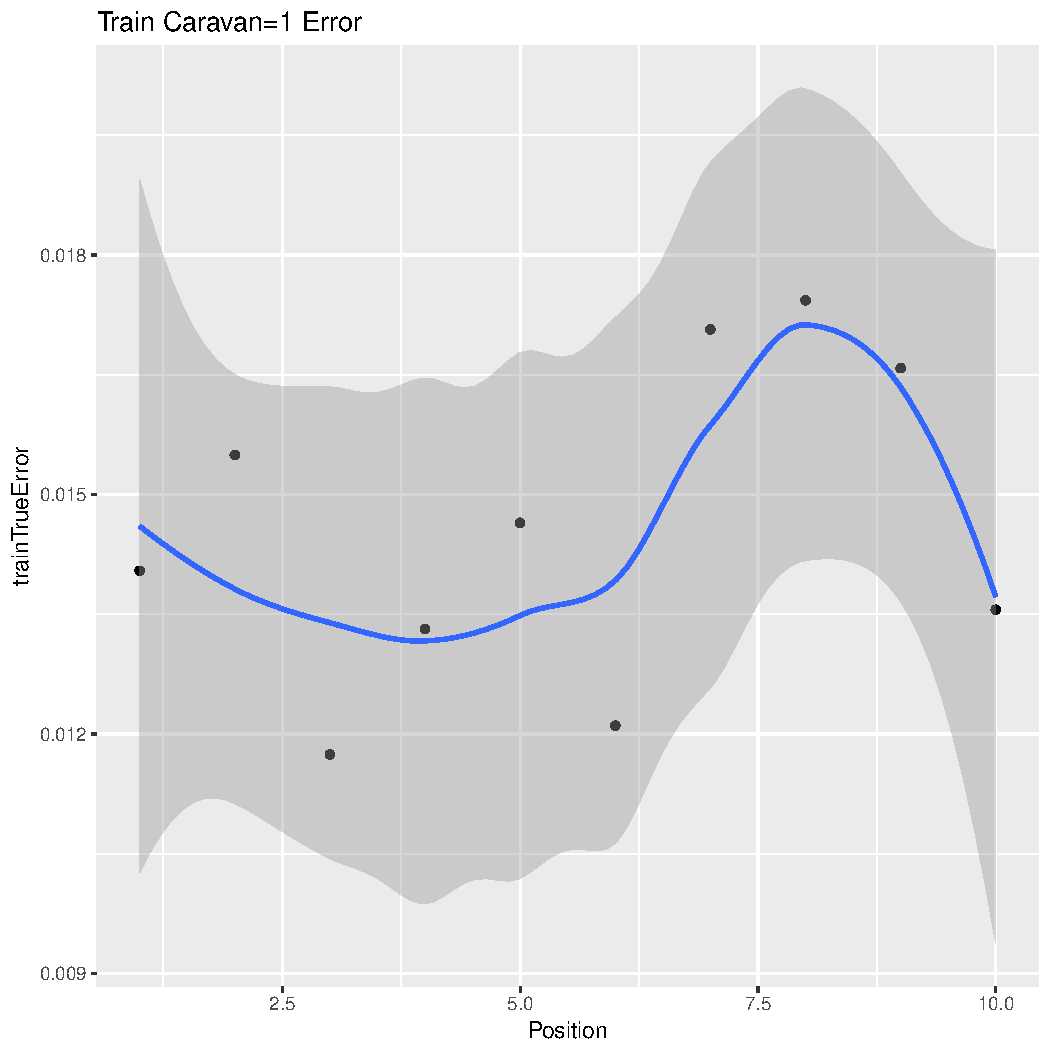
\includegraphics[width=\maxwidth]{figure/unnamed-chunk-43-3} 
\begin{kframe}

{\ttfamily\noindent\itshape\color{messagecolor}{\#\# `geom\_smooth()` using method = 'loess'}}\end{kframe}
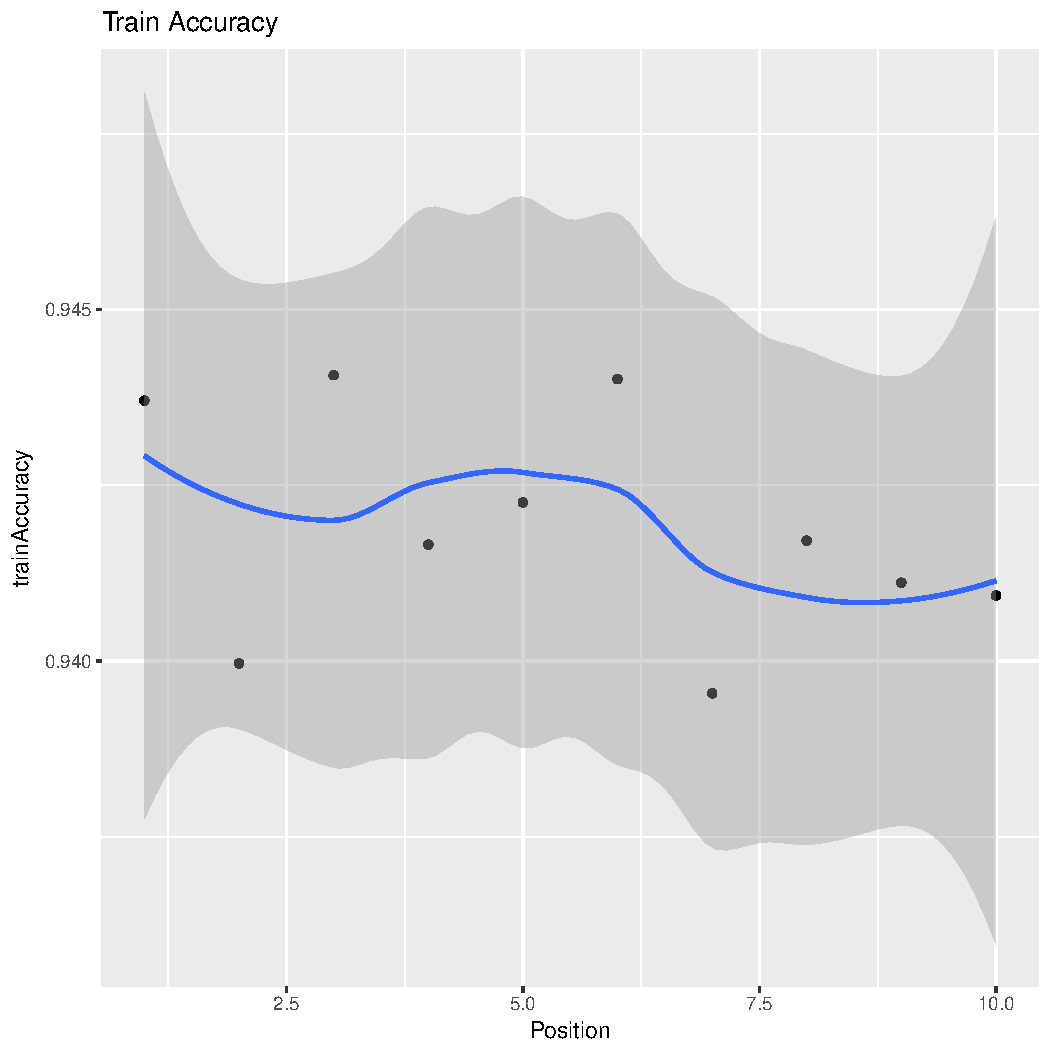
\includegraphics[width=\maxwidth]{figure/unnamed-chunk-43-4} 
\begin{kframe}

{\ttfamily\noindent\itshape\color{messagecolor}{\#\# `geom\_smooth()` using method = 'loess'}}\end{kframe}
\includegraphics[width=\maxwidth]{figure/unnamed-chunk-43-5} 
\begin{kframe}

{\ttfamily\noindent\itshape\color{messagecolor}{\#\# `geom\_smooth()` using method = 'loess'}}\end{kframe}
\includegraphics[width=\maxwidth]{figure/unnamed-chunk-43-6} 
\begin{kframe}

{\ttfamily\noindent\itshape\color{messagecolor}{\#\# `geom\_smooth()` using method = 'loess'}}\end{kframe}
\includegraphics[width=\maxwidth]{figure/unnamed-chunk-43-7} 
\begin{kframe}

{\ttfamily\noindent\itshape\color{messagecolor}{\#\# `geom\_smooth()` using method = 'loess'}}\end{kframe}
\includegraphics[width=\maxwidth]{figure/unnamed-chunk-43-8} 
\begin{kframe}\begin{verbatim}
## [1] "Average OOB: 0.0580025177342746"
## [1] "Average CARAVAN=0 Error: 0.101147961151855"
## [1] "Average CARAVAN=1 Error: 0.0145986364167433"
## [1] "Average Train Accuracy: 0.941895205004096"
## [1] " "
## [1] "Average Test Error: 0.0484385109117277"
## [1] "Average CARAVAN=0 Error: 0.0878174642259149"
## [1] "Average CARAVAN=1 Error: 0.00882352941176471"
## [1] "Average Test Accuracy: 0.951561489088272"
\end{verbatim}
\end{kframe}
\end{knitrout}
During testing, only one column was removed but this did cause an increase in accuracy in both the training and testing accuracies. Error rate averages did slighly decrease, but there was a change in the range of values. Error rates for when CARAVAN=1 dropped, but error rates for CARAVAN=0 rose. In some cases by nearly 20 percent. 
\section{Conclusions}
My model was not very accurate, the real issue being the error rate in predicting when CARAVAN=1. More data would be helpful and I think a better resampling technique such as bootstrap might have helped. A different model such as a neural network might have performed better. By the final model, my model was around 60-62 percent accuracy and error rates for CARAVAN=1 were in the 60-80 percent range. 

I did originally try and remove highly correlated variables, but didn't have much success so I ommited this from the coursework. If I had more time I would retry this to see if It could improve the accuracy.

If I had more time, I would have tried to combine some the variables into new ones. I would have tried to combine the 5 social class variables for example into one variable, and classify each row as one social class. Due to time constraints I was not able to do this. 

I would have also tried to identify more important predictors and great a model with only those predictors. 

I feel like I have learned much completing this coursework despite the fact the accuracy of my model wasn't great. 
\section{References}
\begin{itemize}
  \item Wickham, H(2013). ggplot2.[online] Available at: http://ggplo2.org/ [Accessed 16th Dec 2017]  
  \item Wickham, H(2017). Package 'dplyr' v0.7.4.[PDF] Available at:https://cran.r-project.org/web/packages/dplyr/dplyr.pdf [Accessed: 16th Dec 2017]
  \item Lunardon, N(2014). Package 'ROSE' V0.0-3.[PDF] Available at:https://cran.r-project.org/web/packages/ROSE/ROSE.pdf [Accessed: 16th Dec 2017]
  \item analyticsvidhya,(2016). Practical Guide to deal with Imbalanced Classification Problems in R.[online] Available at:https://www.analyticsvidhya.com/blog/2016/03/practical-guide-deal-imbalanced-classification-problems/ [Accessed: 16th Dec 2017]
  \item Liaw, A(2015). Package 'randomForest' V4.6-12. [PDF] Available at:https://cran.r-project.org/web/packages/randomForest/randomForest.pdf [Accessed: 16th Dec 2017]
  \item topepo,(2017). The caret Package.[online] Available at:http://topepo.github.io/caret/index.html [Accessed 16th Dec 2017]
\end{itemize}
\end{document}
